
\documentclass{article}

%packages
\usepackage{geometry}
\usepackage{listings}
\usepackage[hidelinks]{hyperref}
\usepackage{color}
\usepackage{graphicx}
\usepackage{array,ragged2e}
\usepackage{algorithm}
\usepackage{algorithmic}
\newcolumntype{P}[1]{>{\RaggedRight\arraybackslash}p{#1}}


%setup
\date{}
\title{Maze Generation NEA}
\author{Alexander Noles}
\geometry{margin=0.5in}

\definecolor{mygreen}{rgb}{0,0.6,0}
\definecolor{amber}{rgb}{1.0, 0.49, 0.0}
\definecolor{mywhite}{rgb}{0.95, 0.95, 0.96}
\definecolor{mygrey}{rgb}{0.6, 0.6, 0.6}


\lstset{language=Python,
	backgroundcolor=\color{mywhite}, 
 	 basicstyle=\footnotesize,       
 	 breaklines=true,                 
 	 captionpos=b,                    
  	commentstyle=\color{red},   
 	 escapeinside={\%*}{*)},          
 	 keywordstyle=\color{amber},       
  	stringstyle=\color{mygreen},     
	showstringspaces=false,
	framesep=10pt,
} 
\renewcommand{\arraystretch}{1.7}

\begin{document}

\maketitle
\thispagestyle{empty}



\clearpage\pagenumbering{arabic}

\fontsize{12}{13}\selectfont
\setcounter{tocdepth}{1}
\tableofcontents
 
%%%%%%%%%%%%%%%%%%%%%%%%%%
\clearpage
\part{Analysis}

\section{Research}
\subsection{General Research}
Research on maze generation algorithms was done using the book "Mazes for Programmers", with "Kruskal's algorithim" being the specific algorithim
chosen. It is described as such in the book; "Kruskal's algorithm was developed by the mathematician and computer scientist Joseph Kruskal in 1956 to
construct \emph{minimum spanning trees}." "Basically, Kruskal was trying to solve the following problem. Let's say you start with a graph, or grid, where
every possible passage that might connect neighboring cells is given a cost." "How do you construct a maze from that initial grid whose passages have costs
that sum to the lowest total value? \emph{What's the cheapest tree that can be built?}". Iin the context of maze generation a ``spanning tree'' is analogous to a "perfect maze" or
a maze where any cell can be reached from any other cell. This is useful as it ensures any maze generated is solvable. The word ``minimum'' means that the 
spanning tree is generated in the least expensive way possible, with the cost being calculated using weights attached to each individual corridor between maze
cells. Corridors having weights allows the program to control how the maze generates while still keeping some randomness, avoiding the mazes becoming reptative immediately.
The algorithm also has a tendency to creating hook-like generation patterns, this makes the mazes easier to solve than they actually look, as a lot of possible paths can
be immediately discounted. On a much more general level the maze can be thought of as generating and joining together a bunch of smaller mazes.
\linebreak
\linebreak
In terms of actually rendering the maze/player, during research I found two main options, one, using Pygame or, two, making it myself. The former of the
two would be easier but it would likely run worse than the latter and give me less control over how the rendering worked. The maze itself would exist entirely 
within screen space (the actual pixels on screen), making the implementation simpler regardless of what option is picked. It should also be noted that pygame
doesn't come pre-installed with python, though it is likely a different external library would be needed to make the rendering work if the
second option was chosen.
Ultimately, I went with the second option due to the added control, I decied to use Pillow (a fork of P.I.L) along with tkinter to create the
implementaion.
\\
\subsection{Potential Users Intial Feedback summary}
%Just lie about it lmao
Due to the recent pandemic, I was forced to get potential users from two forces. One, people I already knew, that I had a direct line of communication to, or two, people I could ask questions to on internet forums. This meant no interviews were conducted but I was able to get some general feedback. Said feedback can be summarised into various key points, which are as follows;
\begin{enumerate}
	\item There should be a general pattern to some of the mazes (e.g. diamond, segmented squares)
	\item Non-square mazes would be a good addition, for example, quite a few suggested circles
	\item Input should feel nice, things such as being able to hold down the movement keys to keep moving in a given direction
	\item A custom maze screen that allows you to create very large mazes (even if they would be next to immpossible to complete)
	\item Add music if it was possible for me to do so
	\item One user also suggested a bloom like effect on the walls of the maze
\end{enumerate}

\clearpage
\section{Examples of Maze Games}
\begin{minipage}{0.4\textwidth}
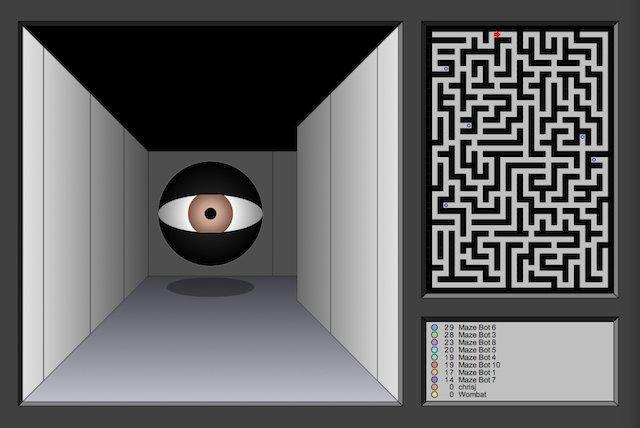
\includegraphics[scale=0.3]{example of old maze}
\end{minipage}
\begin{minipage}{0.5\textwidth}\raggedright
Here is shown an example of a very early maze game, called "Maze War". While the game is mostly played in first-person there is also a top-down map
shown. Thier representation of the maze is seemingly made up of cells that can eithier be walls or non-walls, for my implementation I instead opted to
have each cell have four toggleable walls. 
\end{minipage}
\linebreak
\\
\linebreak
\begin{minipage}{0.4\textwidth}
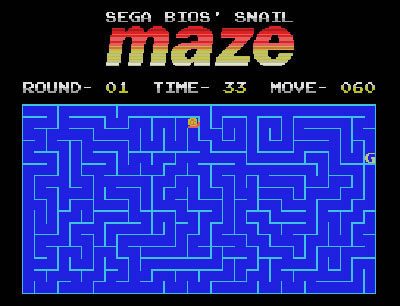
\includegraphics[scale=0.48]{better example}
\end{minipage}
\begin{minipage}{0.5\textwidth}\raggedright
This example is much closer to what I wanted, including the font used (excluding the title) and the way the maze is presented. The only major difference to the way
the maze looks is that my version doesn't include a blue backing. There is also a slight visual glitch where some of the lines of the maze are rendered thicker than others,
which is likely caused by thier renderer not being adjusted for the given screen size.
\end{minipage}
\linebreak
\\
\linebreak
\begin{minipage}{0.4\textwidth}
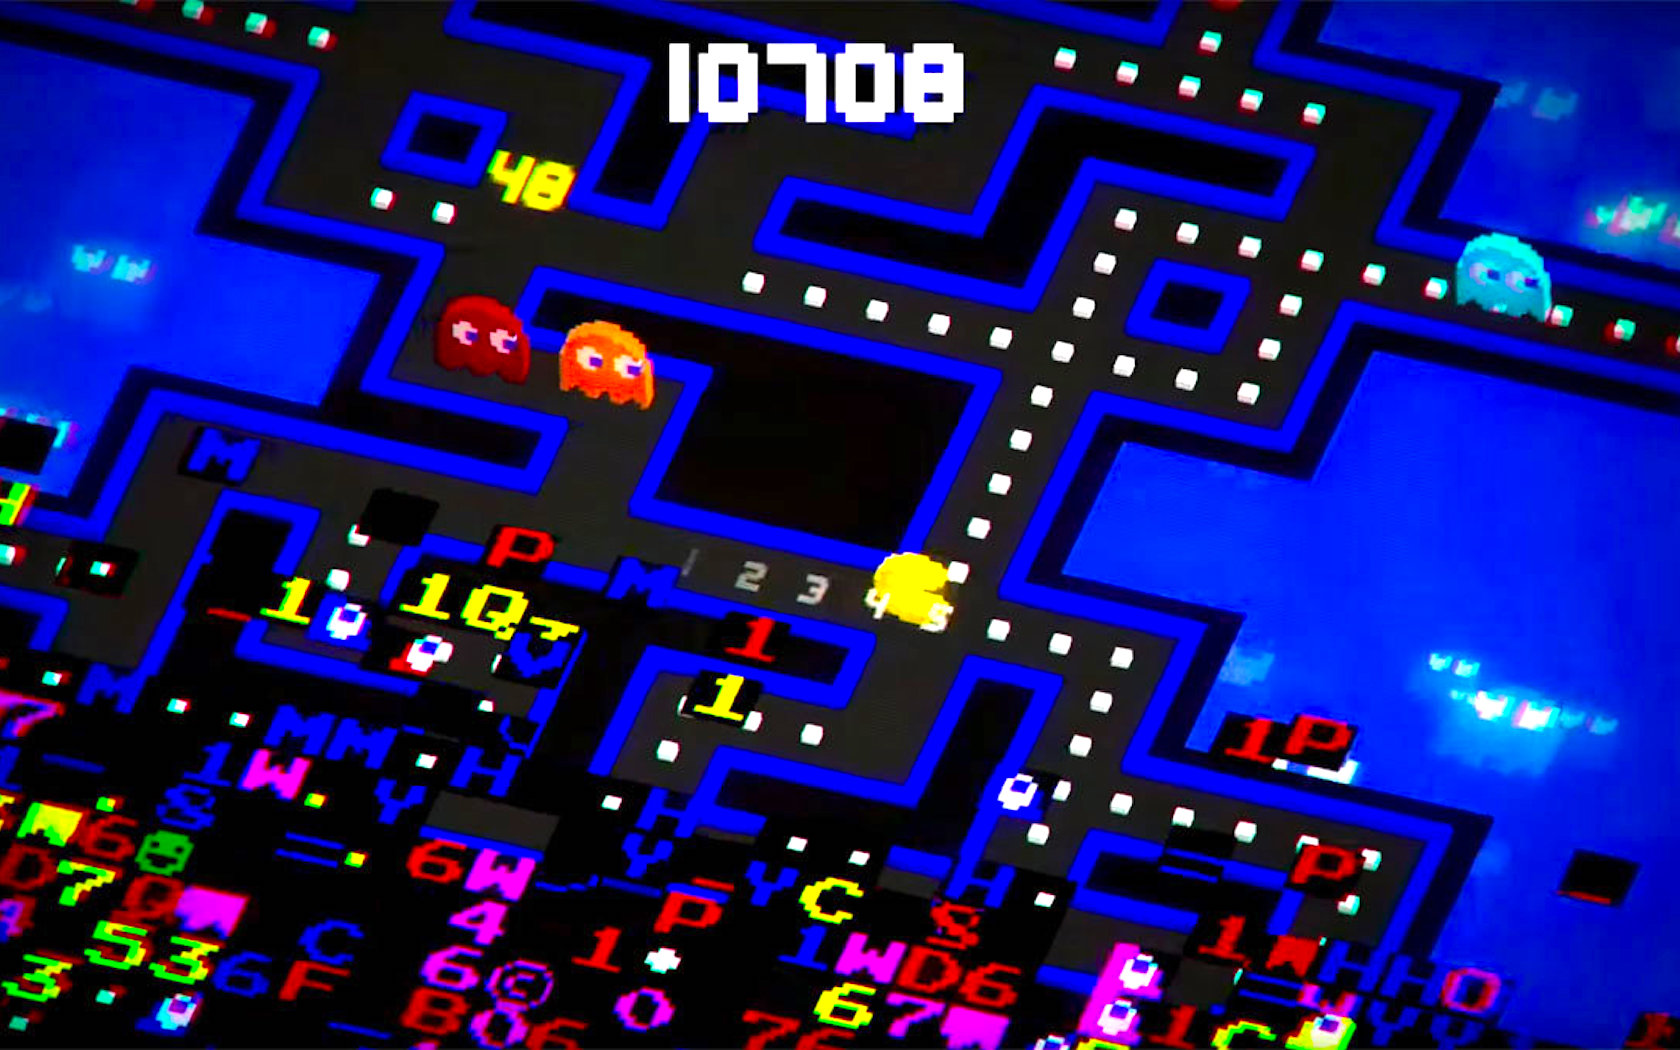
\includegraphics[scale=0.115]{pacman}
\end{minipage}
\begin{minipage}{0.5\textwidth}\raggedright
Pacman is a famous example of a game featuring a maze, however, it differs significantly from the two previous examples. This is true for both the original pacman title and the more modern phone app. In both pressure is put on the player, to make sure they are engaged with the game, this is done through the use ghosts and/or a "wall" that will kill you instantly if it touches you. 
These are both shown in the image on the right. 
\end{minipage}
\linebreak
\\
\linebreak
\begin{minipage}{0.4\textwidth}
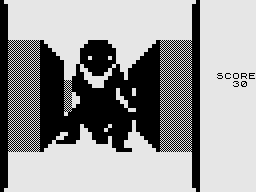
\includegraphics[scale=0.76]{monster maze}
\end{minipage}
\begin{minipage}{0.5\textwidth}\raggedright
Like the first example, the game pictured on the left "3D Monster Maze" is played in first person, however, it lacks the top-down maze view. Similarly to Pac-Man you are hunted, however, there are substantial differences. For example, there is only one monster and, more importatntly, score is gained from surviving rather than picking up dots. Arguably, this game is the furthest from what I want to create but it does a good job of keeping pressure on the player.
\end{minipage}
\linebreak
\\
\linebreak
While having enemies in the maze could be one way of implementing incentive for the player to move through said maze, a timer would probably be an easier solution. In a way this is more similar to the purpose of the wall, limiting the player from spending too long making decisions. However, this isn't a major priority as while it would make the game more fun, it doesn't necessarily showcase any major programming skills that aren't evidenced elsewhere.
\clearpage
\section{Objective Outline}
The point of this project is to create a maze-solving game, fully coded in python. Hence, the objectives are, in order of importance; 
%Add more sub-objectives
\begin{enumerate}
	\item The program must have performative rendering so that the program can run at a sixty frames per second or above (the standard benchmark for modern video games). It should be capable of;
	\begin{enumerate}
		\item Rendering in Layers so that everything on screen doesn't have to be updated every frame
		\item Having any pixel on the screen editable at any given time
	\end{enumerate}
	\item The mazes need to be fully playable and so the system needs to also be capable of;
	\begin{enumerate}
		\item Taking keyboard input 
		\item Detecting if the player is trying to move through a wall and stopping them
		\item Checking to see if the player is at the maze's exit
	\end{enumerate}
	\item The generation of the mazes needs to be controllable while also featuring some form of randomness
	\begin{enumerate}
		\item The data representing the maze also needs to be readable in a way that it can easily be used to implement some of the above features
	\end{enumerate}
	\item A fully functioning GUI will also be needed, including;
	\begin{enumerate}
		\item A screen for selecting the user, that includes the option to create a new user
		\item Another screen for selecting a certain type of maze
		\item As well as a screen for selecting the difficulty or level of the selected maze type
	\end{enumerate}
	\item Finally there should be a system for storing any levels the users have completed
\end{enumerate}

%%%%%%%%%%%%%%%%%%%%%%%%%%
\clearpage
\part{Documented Design}
\section{Program Structure Overview Diagram}
The project will be organized into five scripts, each handiling sections of the project;
\begin{itemize}
\item main.py - Controls/Passes data to the scripts, MazeDatabase, MazeGeneration and MazeRenderer aswell as handiling G.U.I.
\item MazeGeneration.py - Handles maze generations, returning maze\_data arrays that represent mazes.
\item MazeDatabase.py - Controls a user information and completed levels relational database, utilizing SQLite3.
\item Window.py - The previously discussed implementation of tkinter and Pillow to create rendering. It will also handle input attached to the windows it creates.
\item MazeRenderer.py - Handles game logic (such as collision) and implements the Window.py script to display the visuals on screen and control the player.
\end{itemize}
\begin{center}
	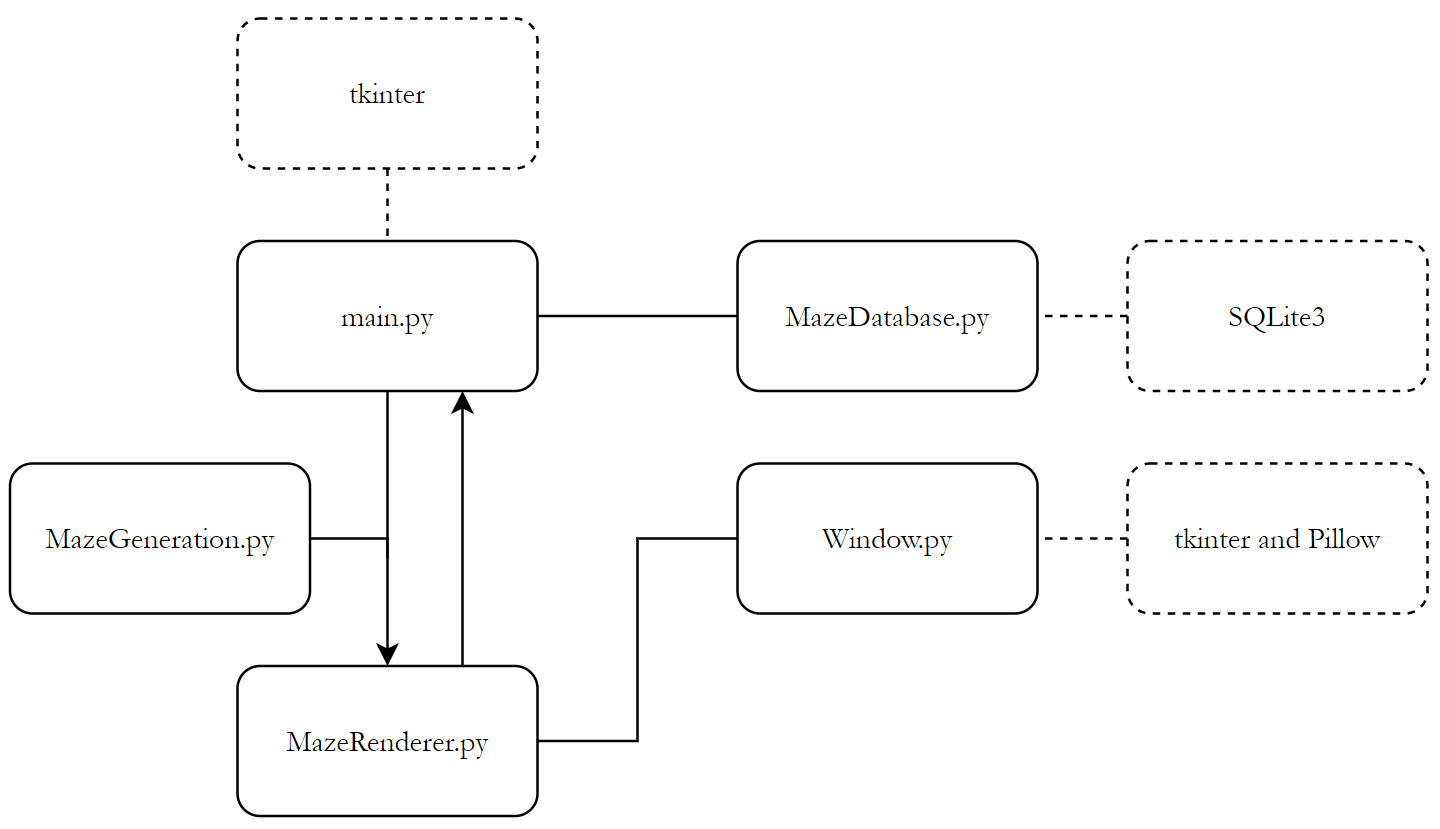
\includegraphics[scale=0.5]{Code Organization Diagram}
\end{center}
Above is a diagram showcasing all the scripts listed in the Organization of Solution section. "main.py" is the starting point, which will also communicate with "MazeDatabase.py"
to handle users/saving completed levels. It also has a link to tkinter, though in the diagram the link is dotted as while tkinter is vital to "main.py" script it is not code I have written.
This is the same relationship with "MazeDatabase.py" and SQLite3. The final link is to "MazeRenderer.py", however, the link itself is connected to "MazeGeneration.py" this is because
while "MazeGeneration.py" is controlled by "main.py" the generated maze is immediately passed to "MazeRenderer.py".
"MazeRenderer.py" has a link to "Window.py" which it uses to create the window of editable pixels used to render the game. There is also a link back to "main.py" as the user
is returned there after the level is completed or quit. "Window.py" also has a dotted link to tkinter and Pillow for the same reason as "main.py" and "MazeDatabase.py" mentioned above.
\clearpage

\section{Database Diagrams}
%Justify use of relational database
To complete my objective of storing a given users completed levels I decided to use a relational database. My justification for this is two-fold, one, I wanted to demonstrate my ability
to use SQLite3 and, two, relational databases allow for a lot more flexibilty/ease-of-use comparaed to storing all of the different users completed levels in a text file.
\subsection{Tables}
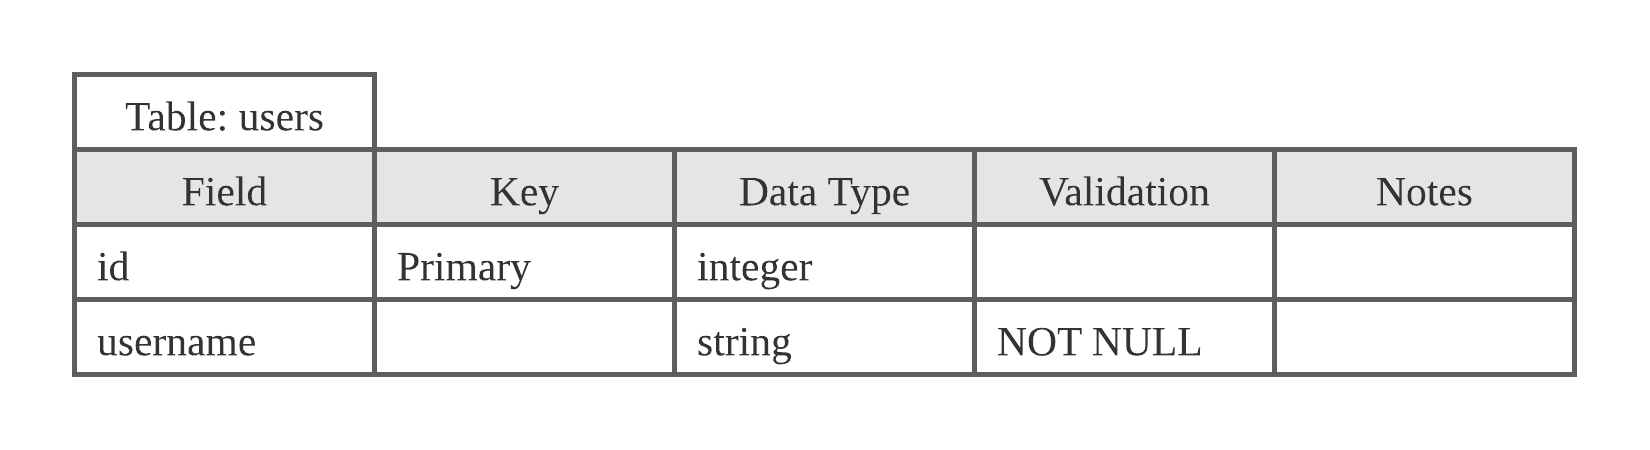
\includegraphics[scale=1]{Users Table}
\linebreak
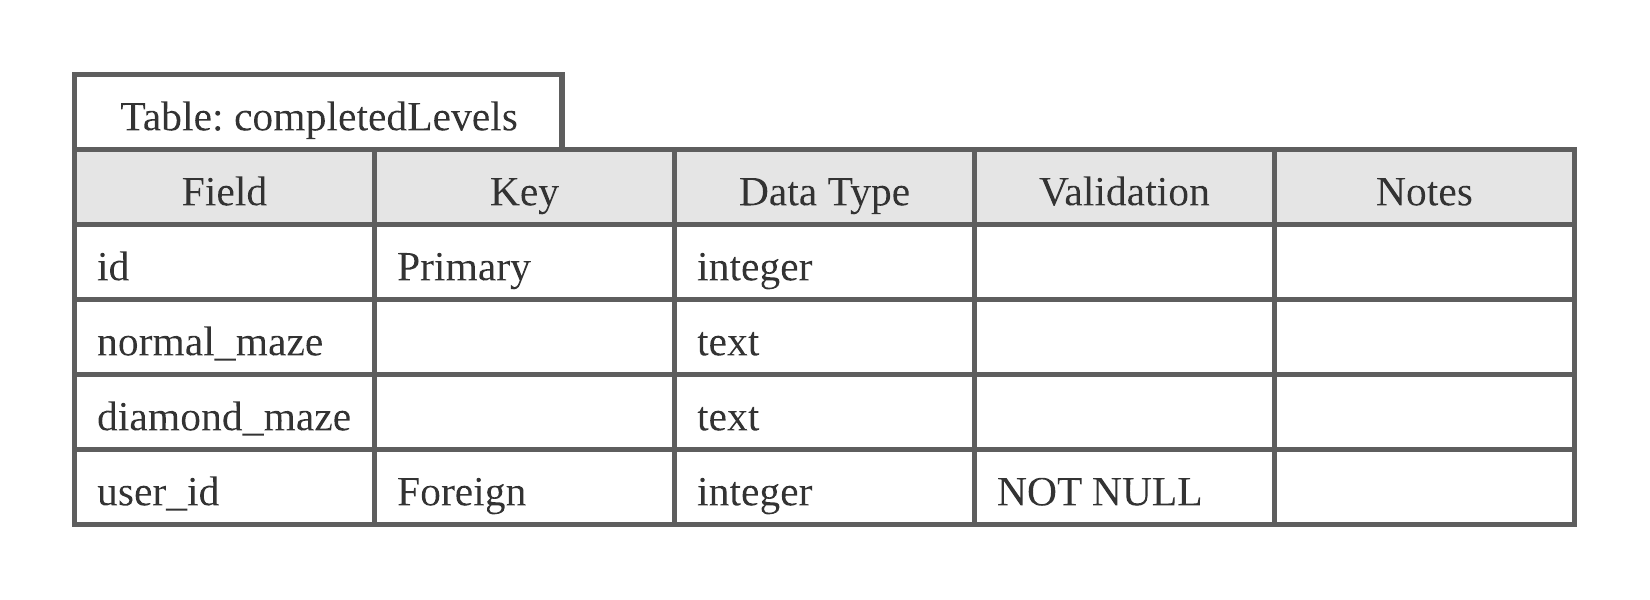
\includegraphics[scale=1]{completedLevels Table}
\linebreak
The fields "normal\_maze" and "diamond\_maze" are both meant to be lists,  however, you are unable to properly store lists in a database. Hence, they must be converted into
text and then also, consequently, be converted back into lists when they need to be accessed. For example, the array [1,2,3,4,5] is converted to '1\#2\#3\#4\#5' by
iterating through the list and appending each entry to a string. The '\#' would also be appended unless the entry is the last one in the array. To convert back to an array a simple
.split('\#') is used on the string.

\subsection{Entity-Relationship Diagram}
\begin{center}
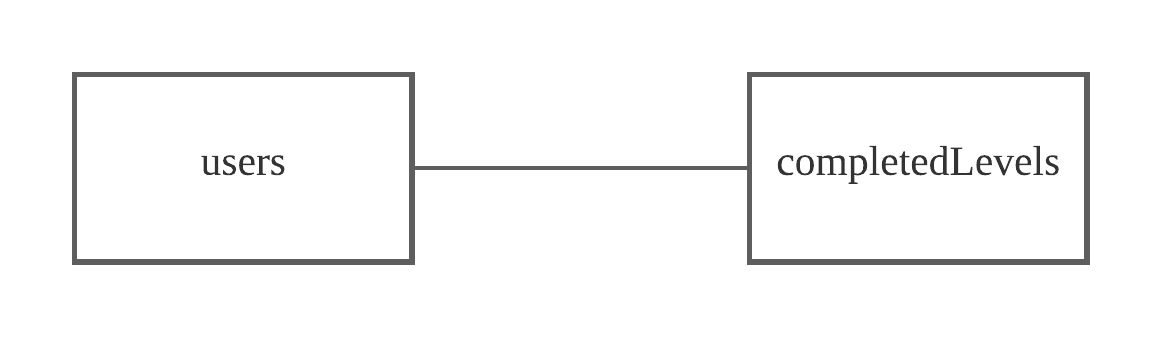
\includegraphics[scale=1]{Database E-R Diagram}
\end{center}
The entity-relationship diagram for the database is very simple as the database itself is simple. There is only one relationship, a one-to-one, between users and completedLevels.
This represents the foreign key user\_id, and is used to link a user's completed levels to them.

\clearpage

\section{Class Diagrams}
%Write explanations of why these exist/how they are used
\subsection{Window}
\begin{center}
	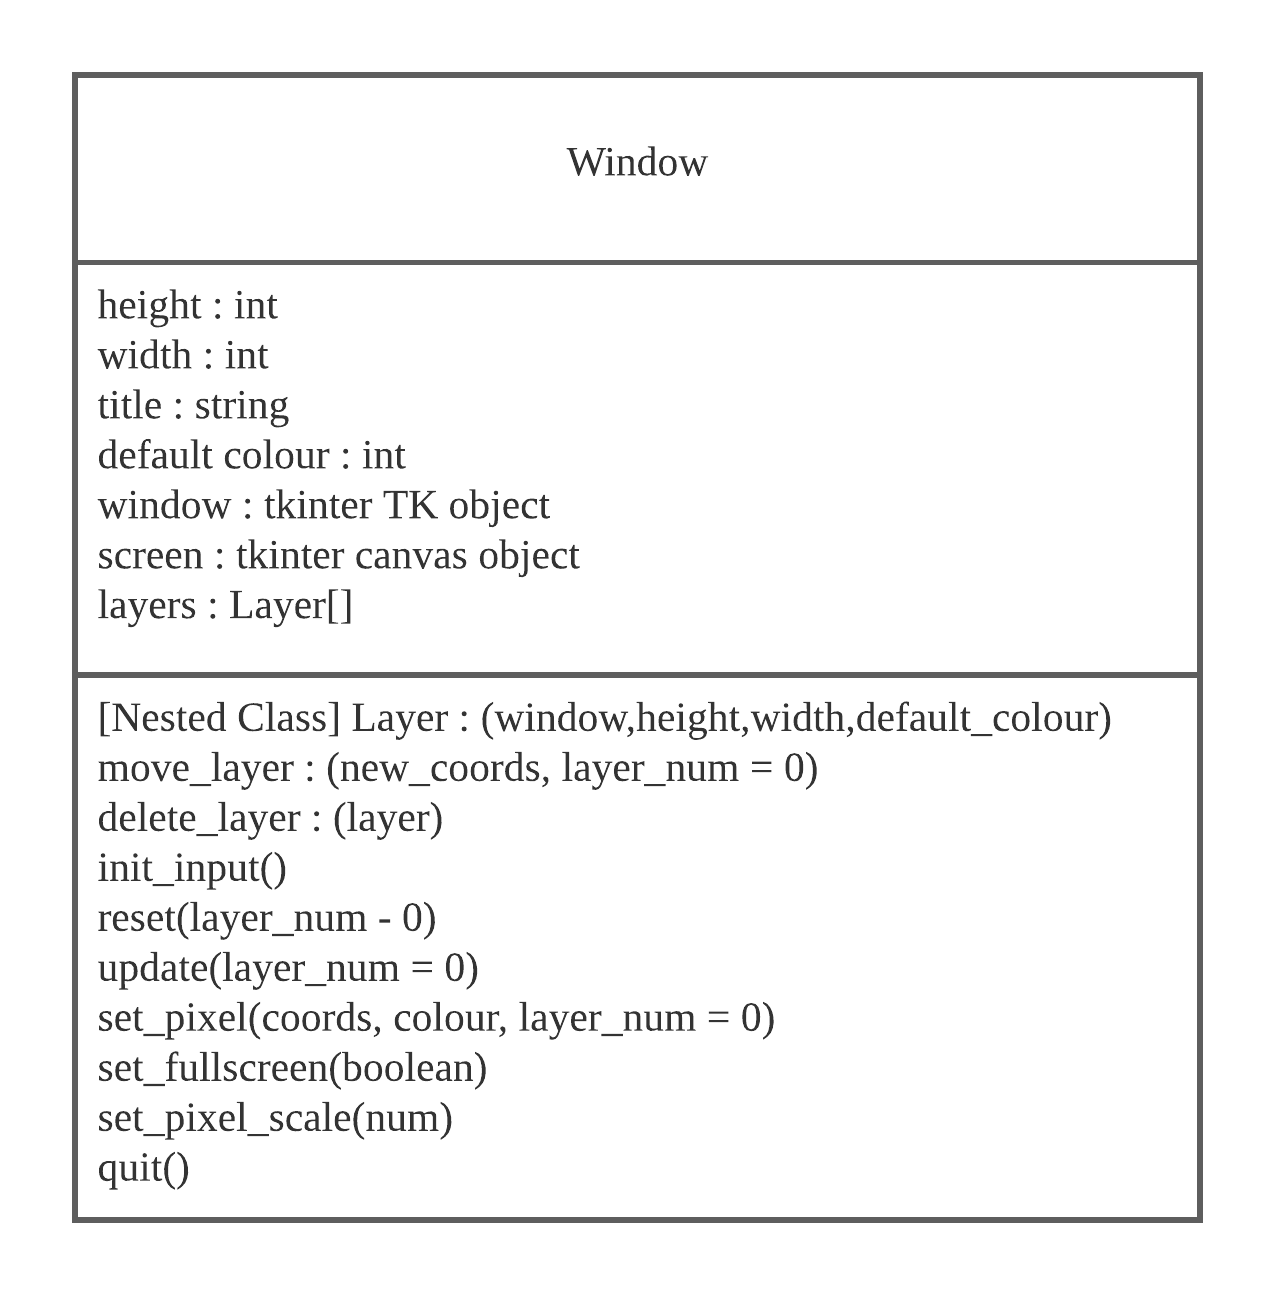
\includegraphics[scale=1]{Window Class}
\end{center}
\subsection{Layer}
\begin{center}
	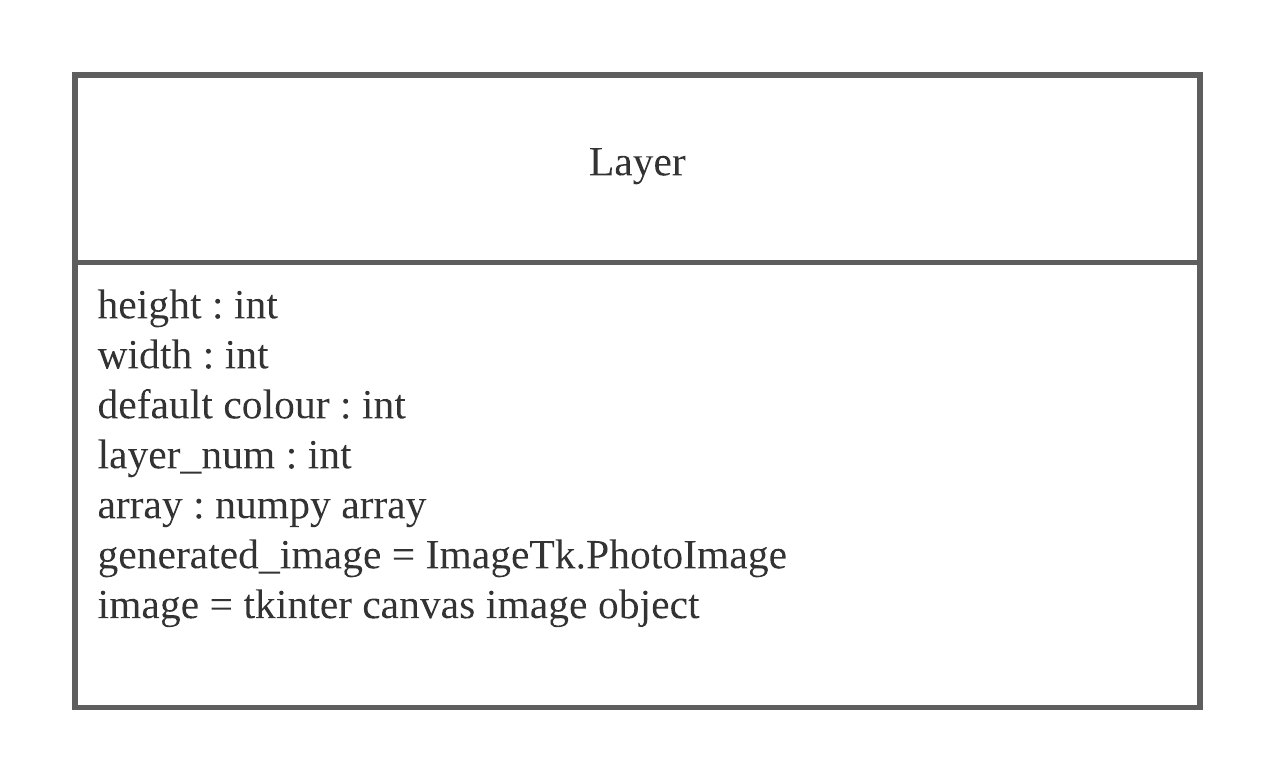
\includegraphics[scale=1]{Layer Class}

	\color{mygrey}(Note: In Python a nested class doesn't imply any relationship)
\end{center}

\clearpage

\section{Algorithms}
\subsection{Kruskals Algorithm Flowchart}
\begin{center}
	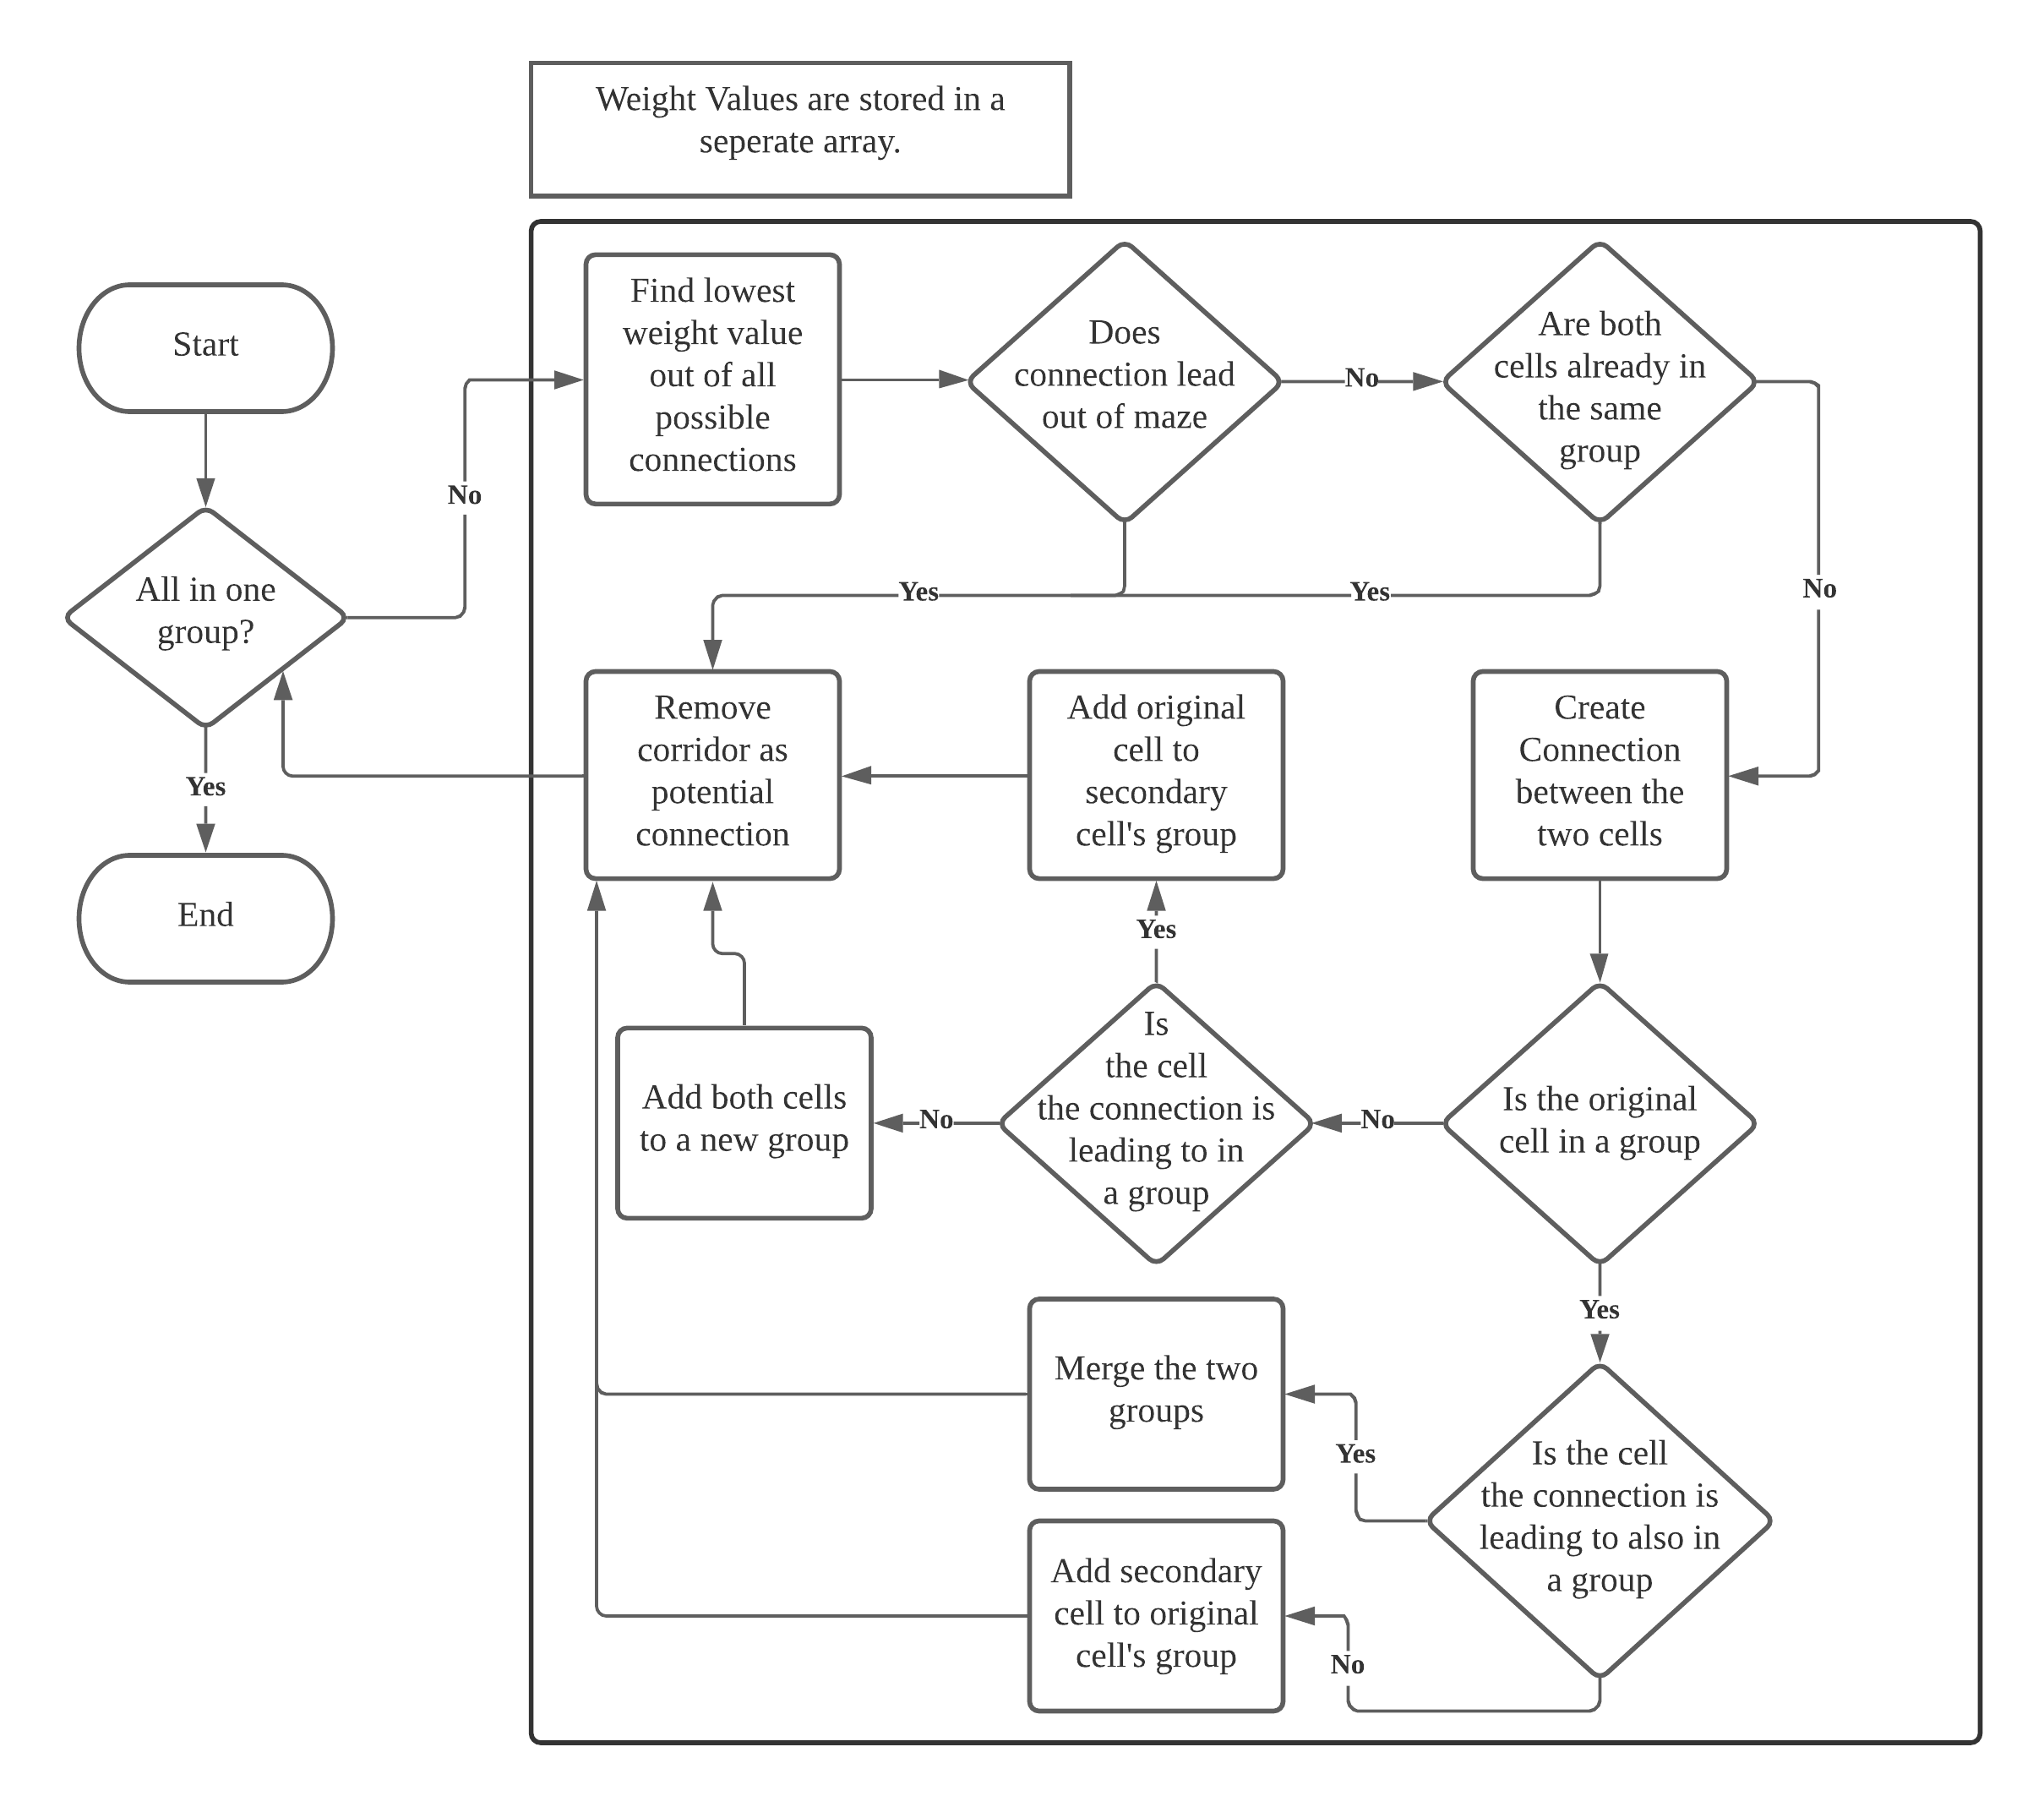
\includegraphics[scale=0.97]{Kruskals}
\end{center}
"Kruskals Algorithim" is the algorithim used to actually generate the mazes. It does this utilizing a \textbf{weight\_group\_array} and by altering
the corridors between cells in the \textbf{maze\_array}. The outline of how it works is this; All cells have a group, at the start this is the default group (i.e. zero).
Any cell within a group is reachable by any other cell in a group (unless it is the default group), they are essentially perfect mazes within the larger maze.
At the start of each iteration of the while loop the code finds corridors (connections between cells) based on the lowest weight, this is done using the afformentioned
\textbf{weight\_group\_array}.
\clearpage
\subsection{Psuedocode for important algorithm}
\subsubsection{Create Level Screen}
\begin{algorithm}
\caption{create\_levels (lower,upper,number of columns,title,array of completed levels)}
\begin{algorithmic} 
\STATE \textbf{FUNC} remove all current GUI elements
\STATE set current button row/y-coordinate as first
\STATE instantiate title
\STATE $i \leftarrow 0$
\FORALL{in range between lower and upper+1 bound}
\STATE$ button\_text \leftarrow i$
\STATE $i \leftarrow +1$
\IF{Level has already been completed}
\STATE Set button text to green
\ELSE
\STATE Set button text to black
\ENDIF
\STATE instantiate button
\IF{i\%number of columns}
\STATE set current button row as next row
\ENDIF
\ENDFOR
\end{algorithmic}
\end{algorithm}
\vphantom{0}
\\
The above function is explained in Psuedocode as it should be the only part of the GUI code that requires much more than simple instantiation of GUI elements.  


\subsubsection{Create a standard weight array}
\begin{algorithm}
\caption{generate\_normal\_weight\_array (height,width, max weight)}
\begin{algorithmic} 
\STATE $weight\_array \leftarrow [ ]$
\STATE $x \leftarrow 0$
\STATE $y \leftarrow 0$
\FORALL{in range between 0 and width}
\STATE $weight\_array.append \leftarrow [ ]$
\FORALL {in range between 0 and height}
\STATE $weight\_array.append \leftarrow$ [4 random numbers between 1 and max\_weight as well as the defualt group]
\STATE $y \leftarrow +1$
\ENDFOR
\STATE $x \leftarrow +1$
\ENDFOR
\RETURN weight\_array
\end{algorithmic}
\end{algorithm}
\vphantom{0}
\\
The above function is an example of a way to create a standard weight array that could be used in the kruskals algorithm shown in the flowchart above.

\clearpage
\section{Data Structures}
\subsection{Maze Array}
A "maze array" is a data structrue meant to represent the maze and is essentially a 2D array. Each cell in the maze has a coordinate and this corresponds to an index in one of the arrays,
meaning each 1D array is equivalent to a row of maze cells. Stored within each actual cell is four integers, which can eithier be one or zero and these represent a wall or a lack of a wall
respectively. A possible optimization would be for these cells to only contain information about the top and left walls as this would still represent almost every wall in the maze, apart from
the very edges on the bottom and right. Given the player isn't able to walk outside of the maze anyway they could simply be replaced with a two lines. The maze array is output by the 
"MazeGeneration.py" script before being transferred to "MazeRenderer.py" where the maze is then shown on screen.
\begin{center}
	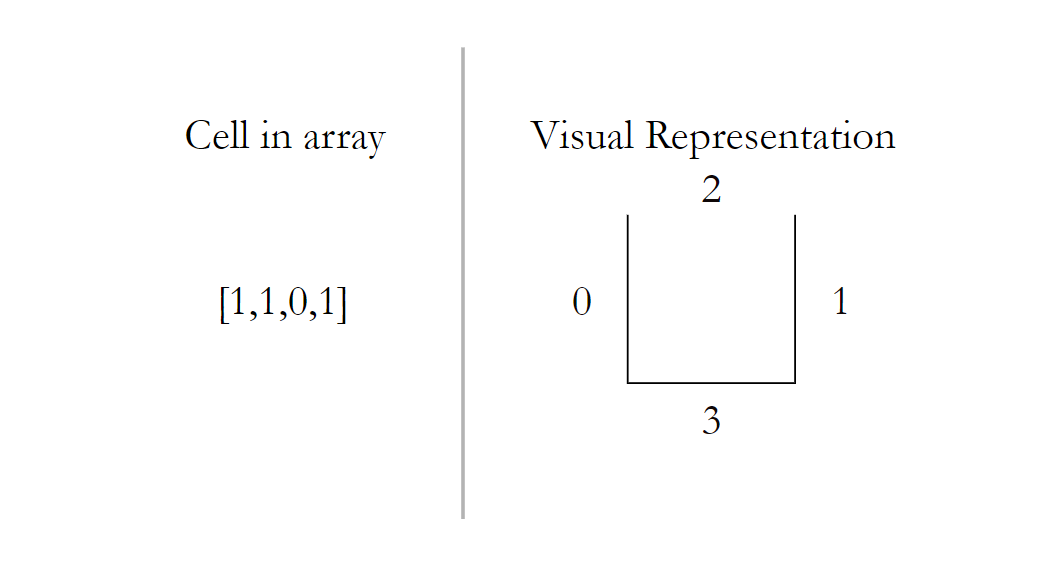
\includegraphics[scale=0.5]{Maze Cell Diagram}

	\color{mygrey}(The numbers on the Visual Representation correlate to the index in the array)
\end{center}
\subsection{Weight Array}
A "weight array" is a very similar data structure to the maze array as it its also a 2D array. Each index in the maze array has a corresponding index in the weight array, they are only kept
in seperate arrays as the data in the weight array does not need to be passed onto "MazeRenderer.py". For every cell wall there is a weight value stored, in the same way walls are stored in 
the "maze array", however, there is also a "group" integer stored with every cell. This group value is used in the Krusklas algorithm used for maze generation and is set to a default/ignored group before maze
generation is run. Having this ignored group is important as it allows the check to see if every cell is in one group to not return true before any alterations have been made to
the maze.

\clearpage
\section{G.U.I }
\subsection{Maze and User Selection}
\begin{center}
%Start Screen
	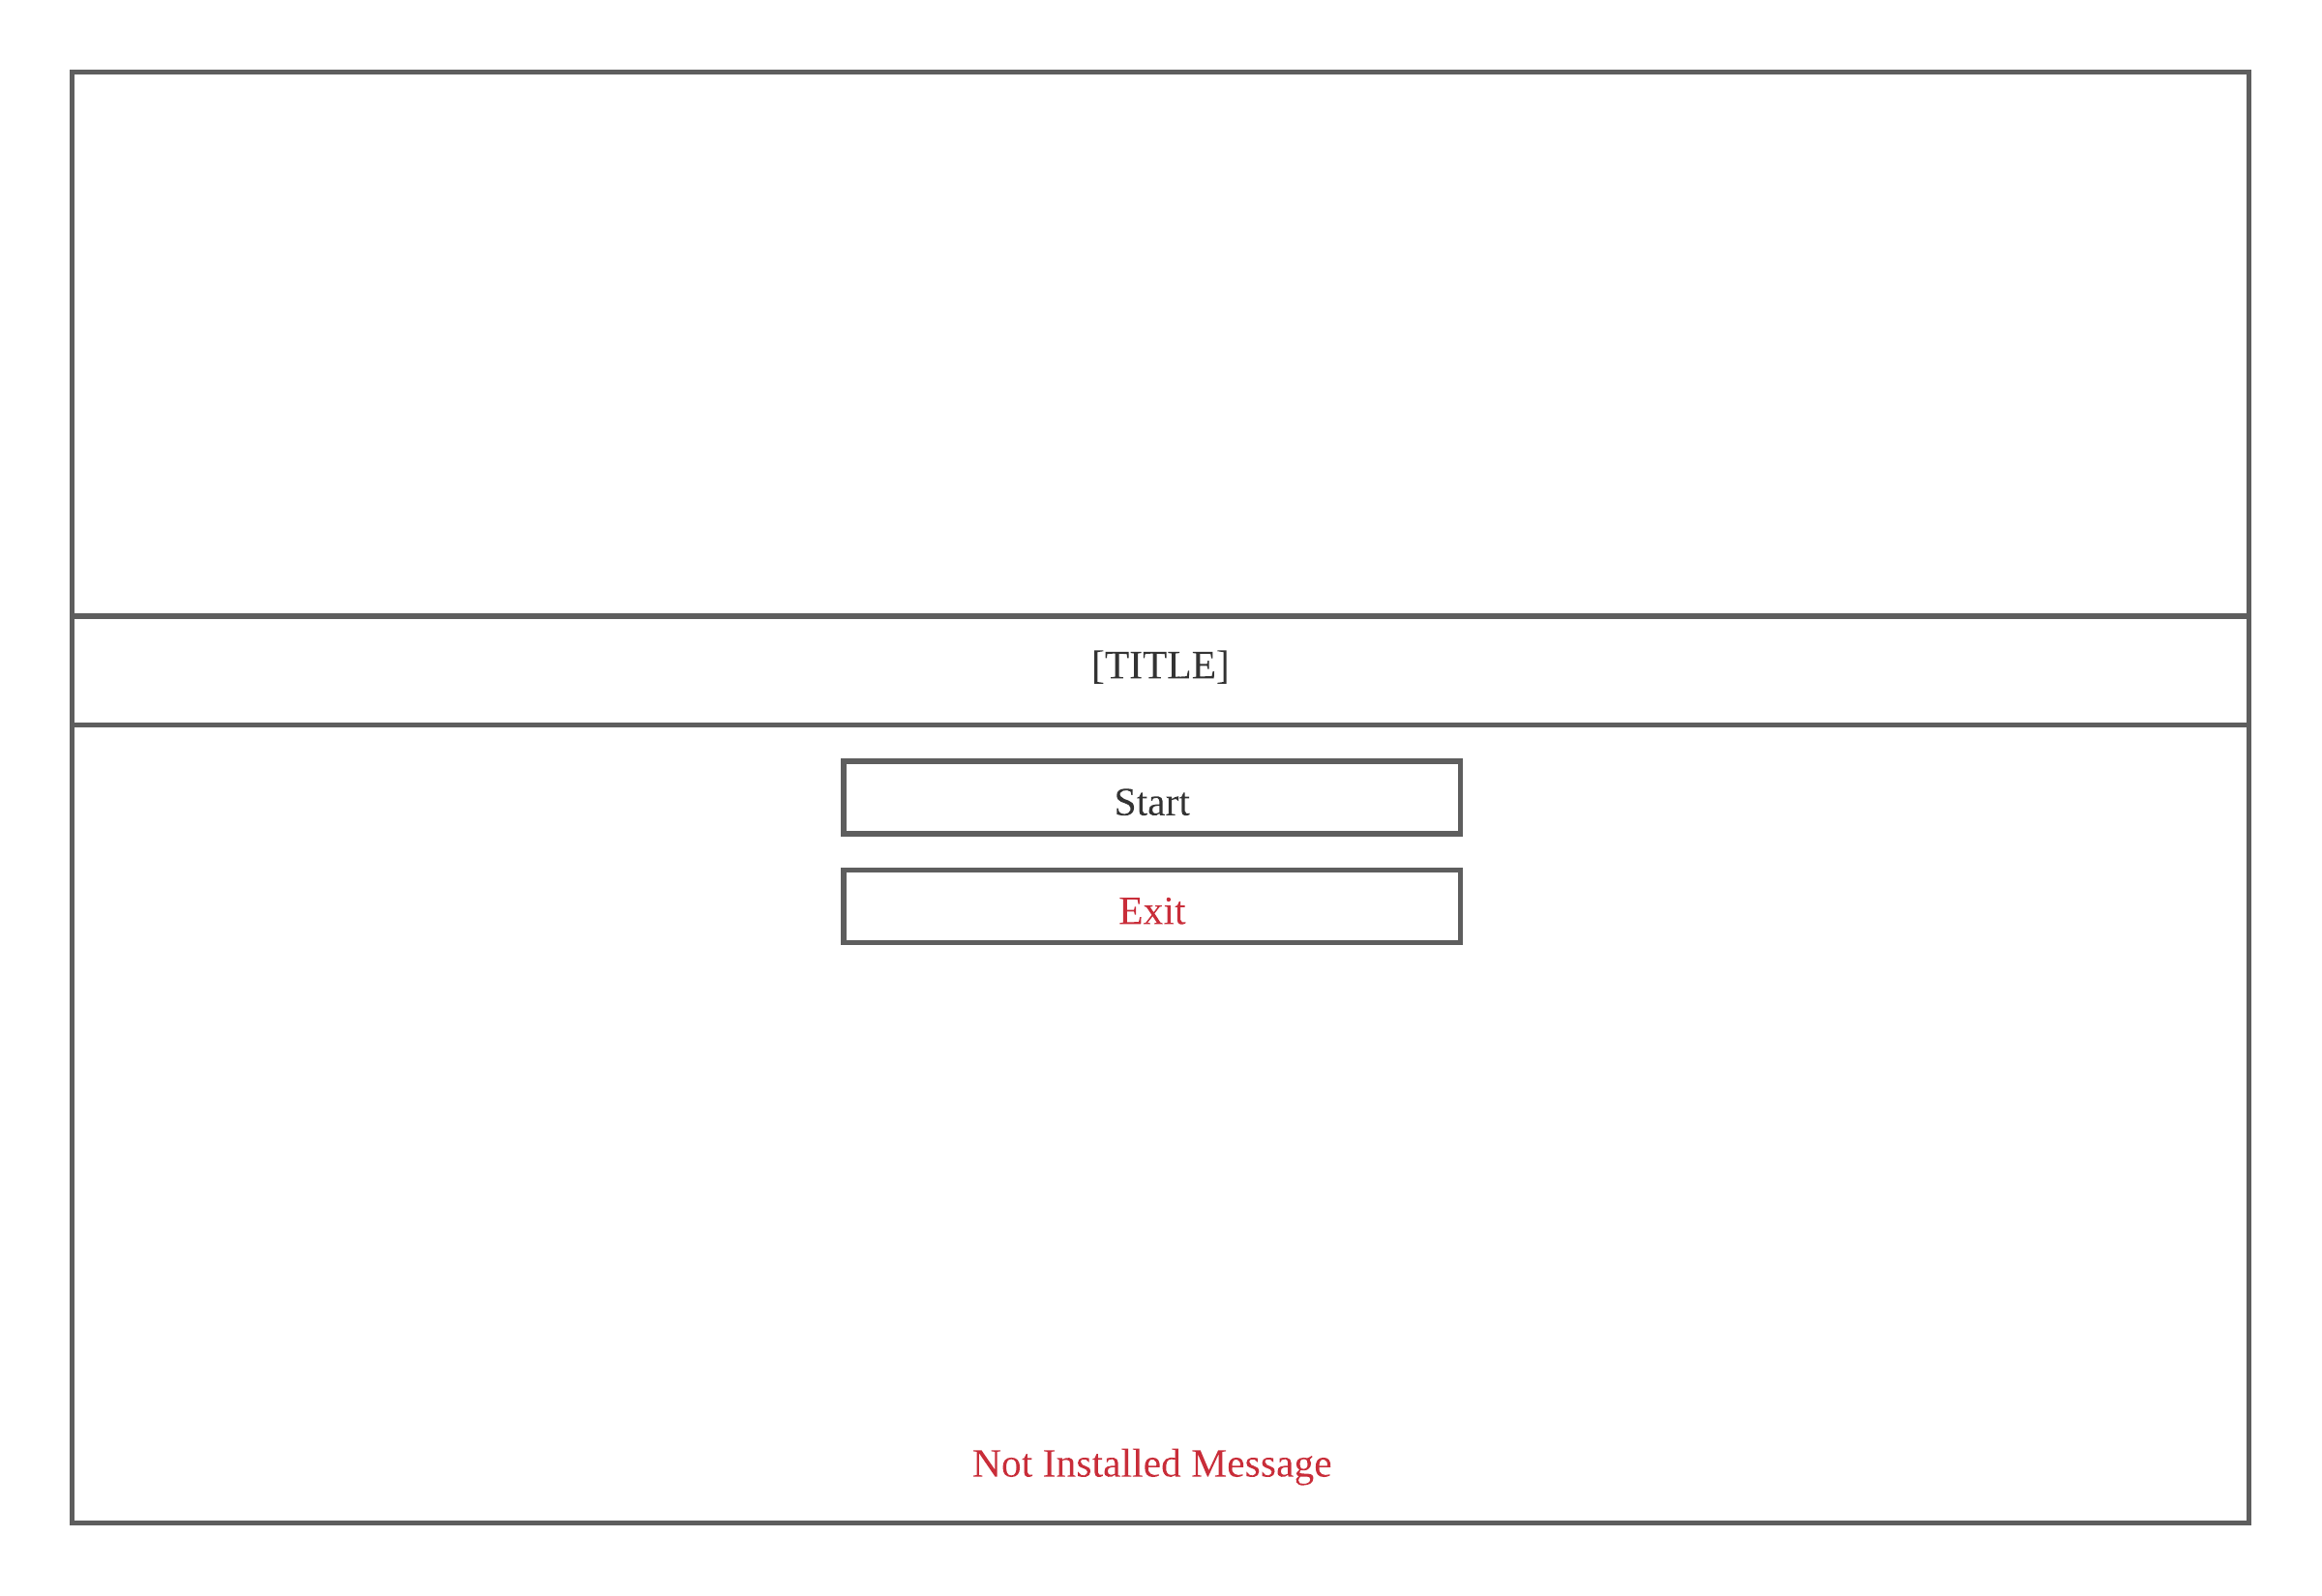
\includegraphics[scale=0.7]{Start Screen}

	Above is the start screen, it features the title and two buttons. The first button is the start button which will lead to the user select
	screen and the second is the exit button which will simply close the button.
\end{center}
\begin{center}
%User Select Screen
	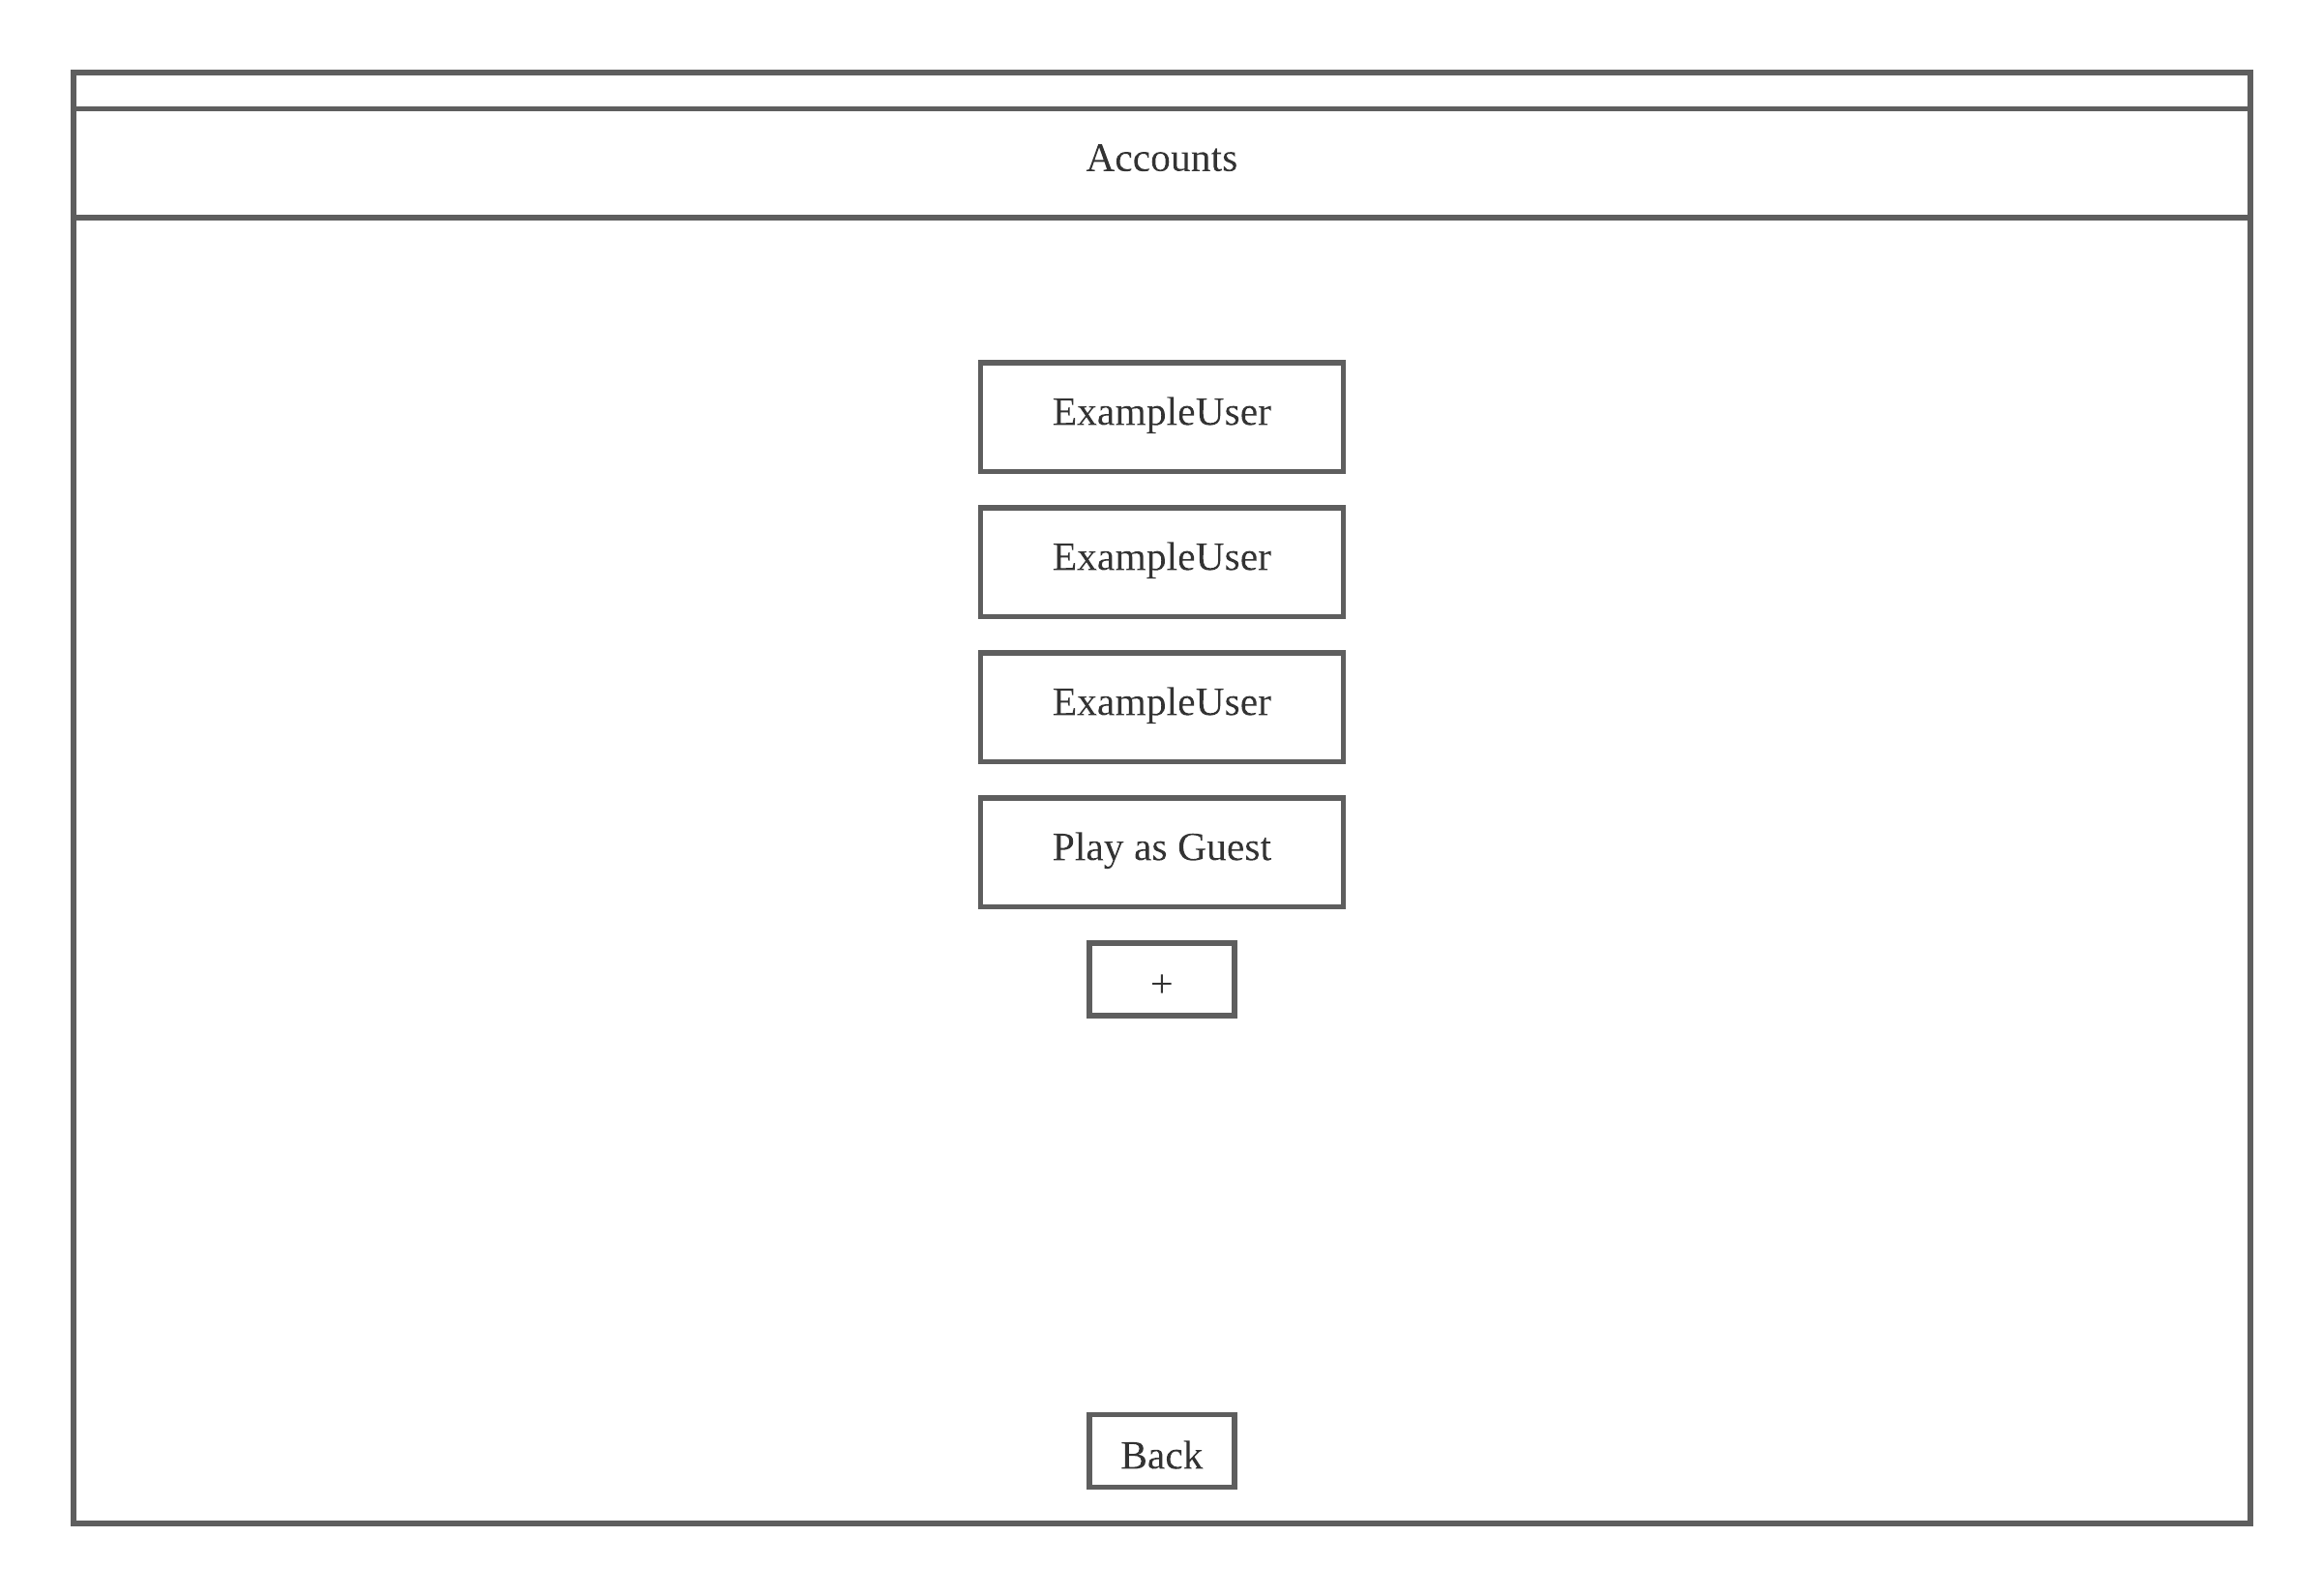
\includegraphics[scale=0.7]{User Select Screen}

	On the user select screen there is a list of created users, a play as guest button, a button to add a new user (the plus) and a back button. The back button
	will send that user back to the start screen.
\end{center}

\begin{center}
%New User Screen
	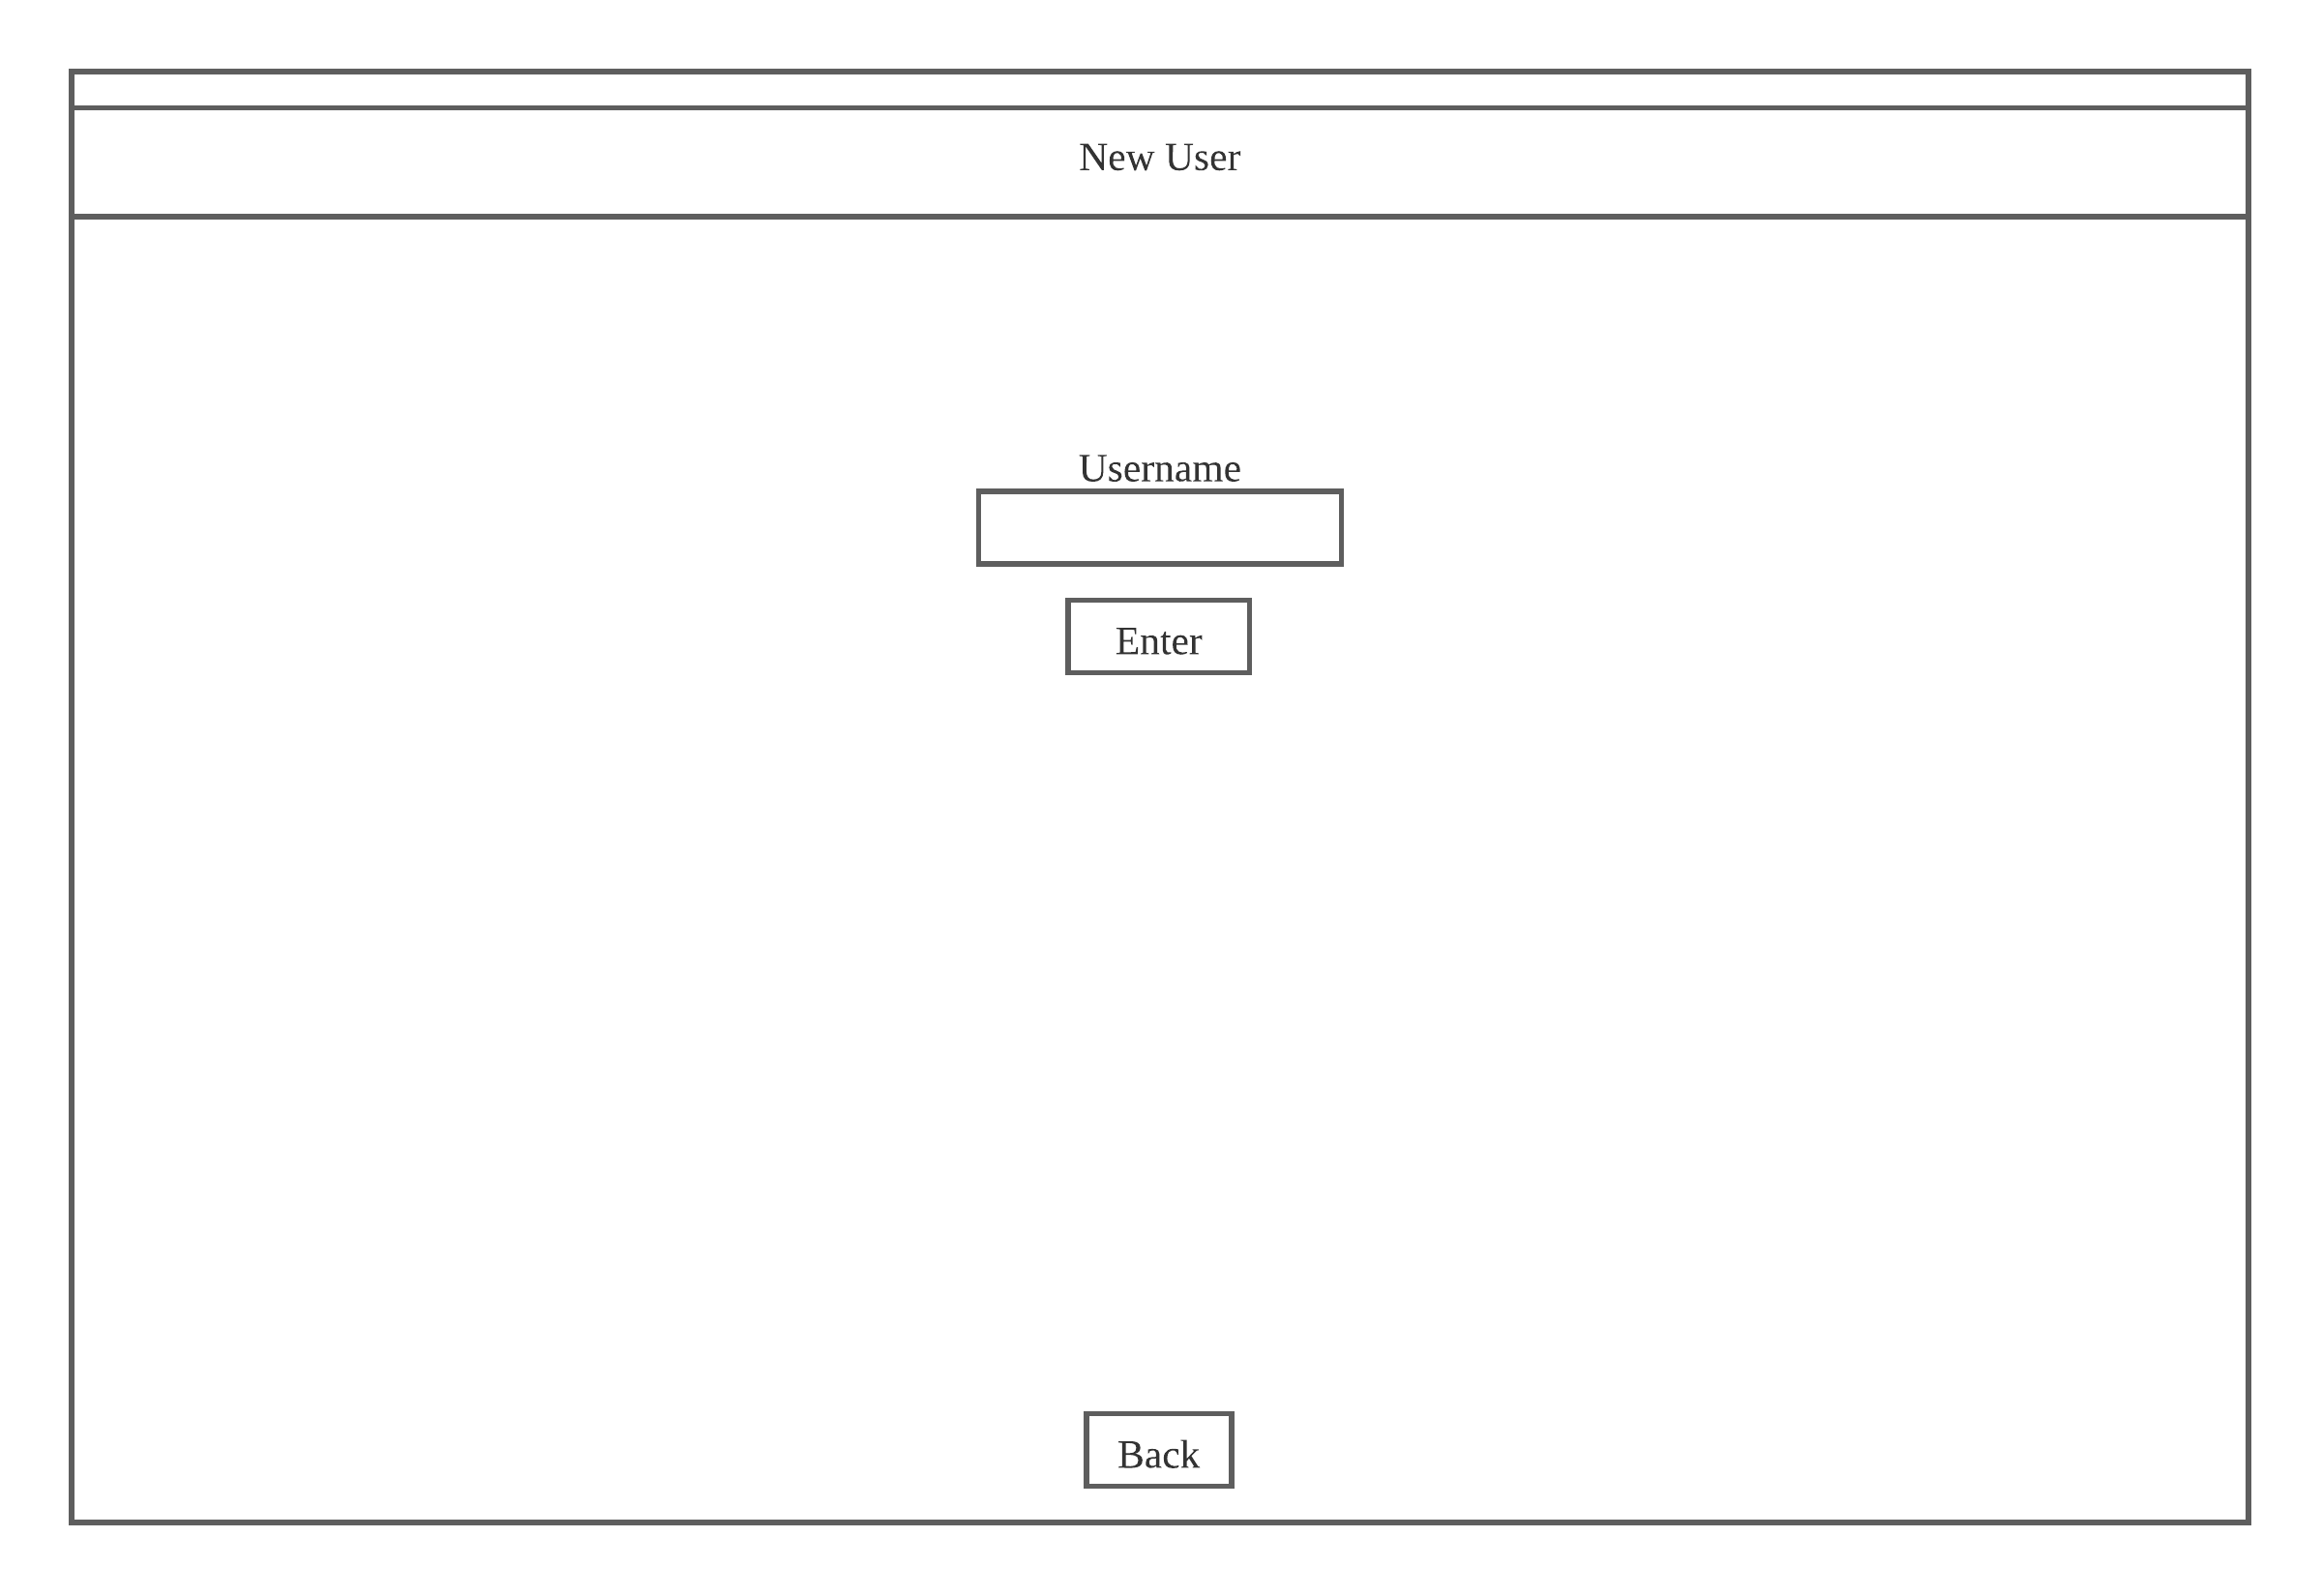
\includegraphics[scale=0.7]{New User Screen}

	The new user screen only needs to include an entry bar for the name to be typed in, a button to confirm the username and a back button (to take the user back to the
	user select screen). There is exception handiling to stop a username being entered that is blank.
\end{center}

\begin{center}
%Maze type Select Screen
	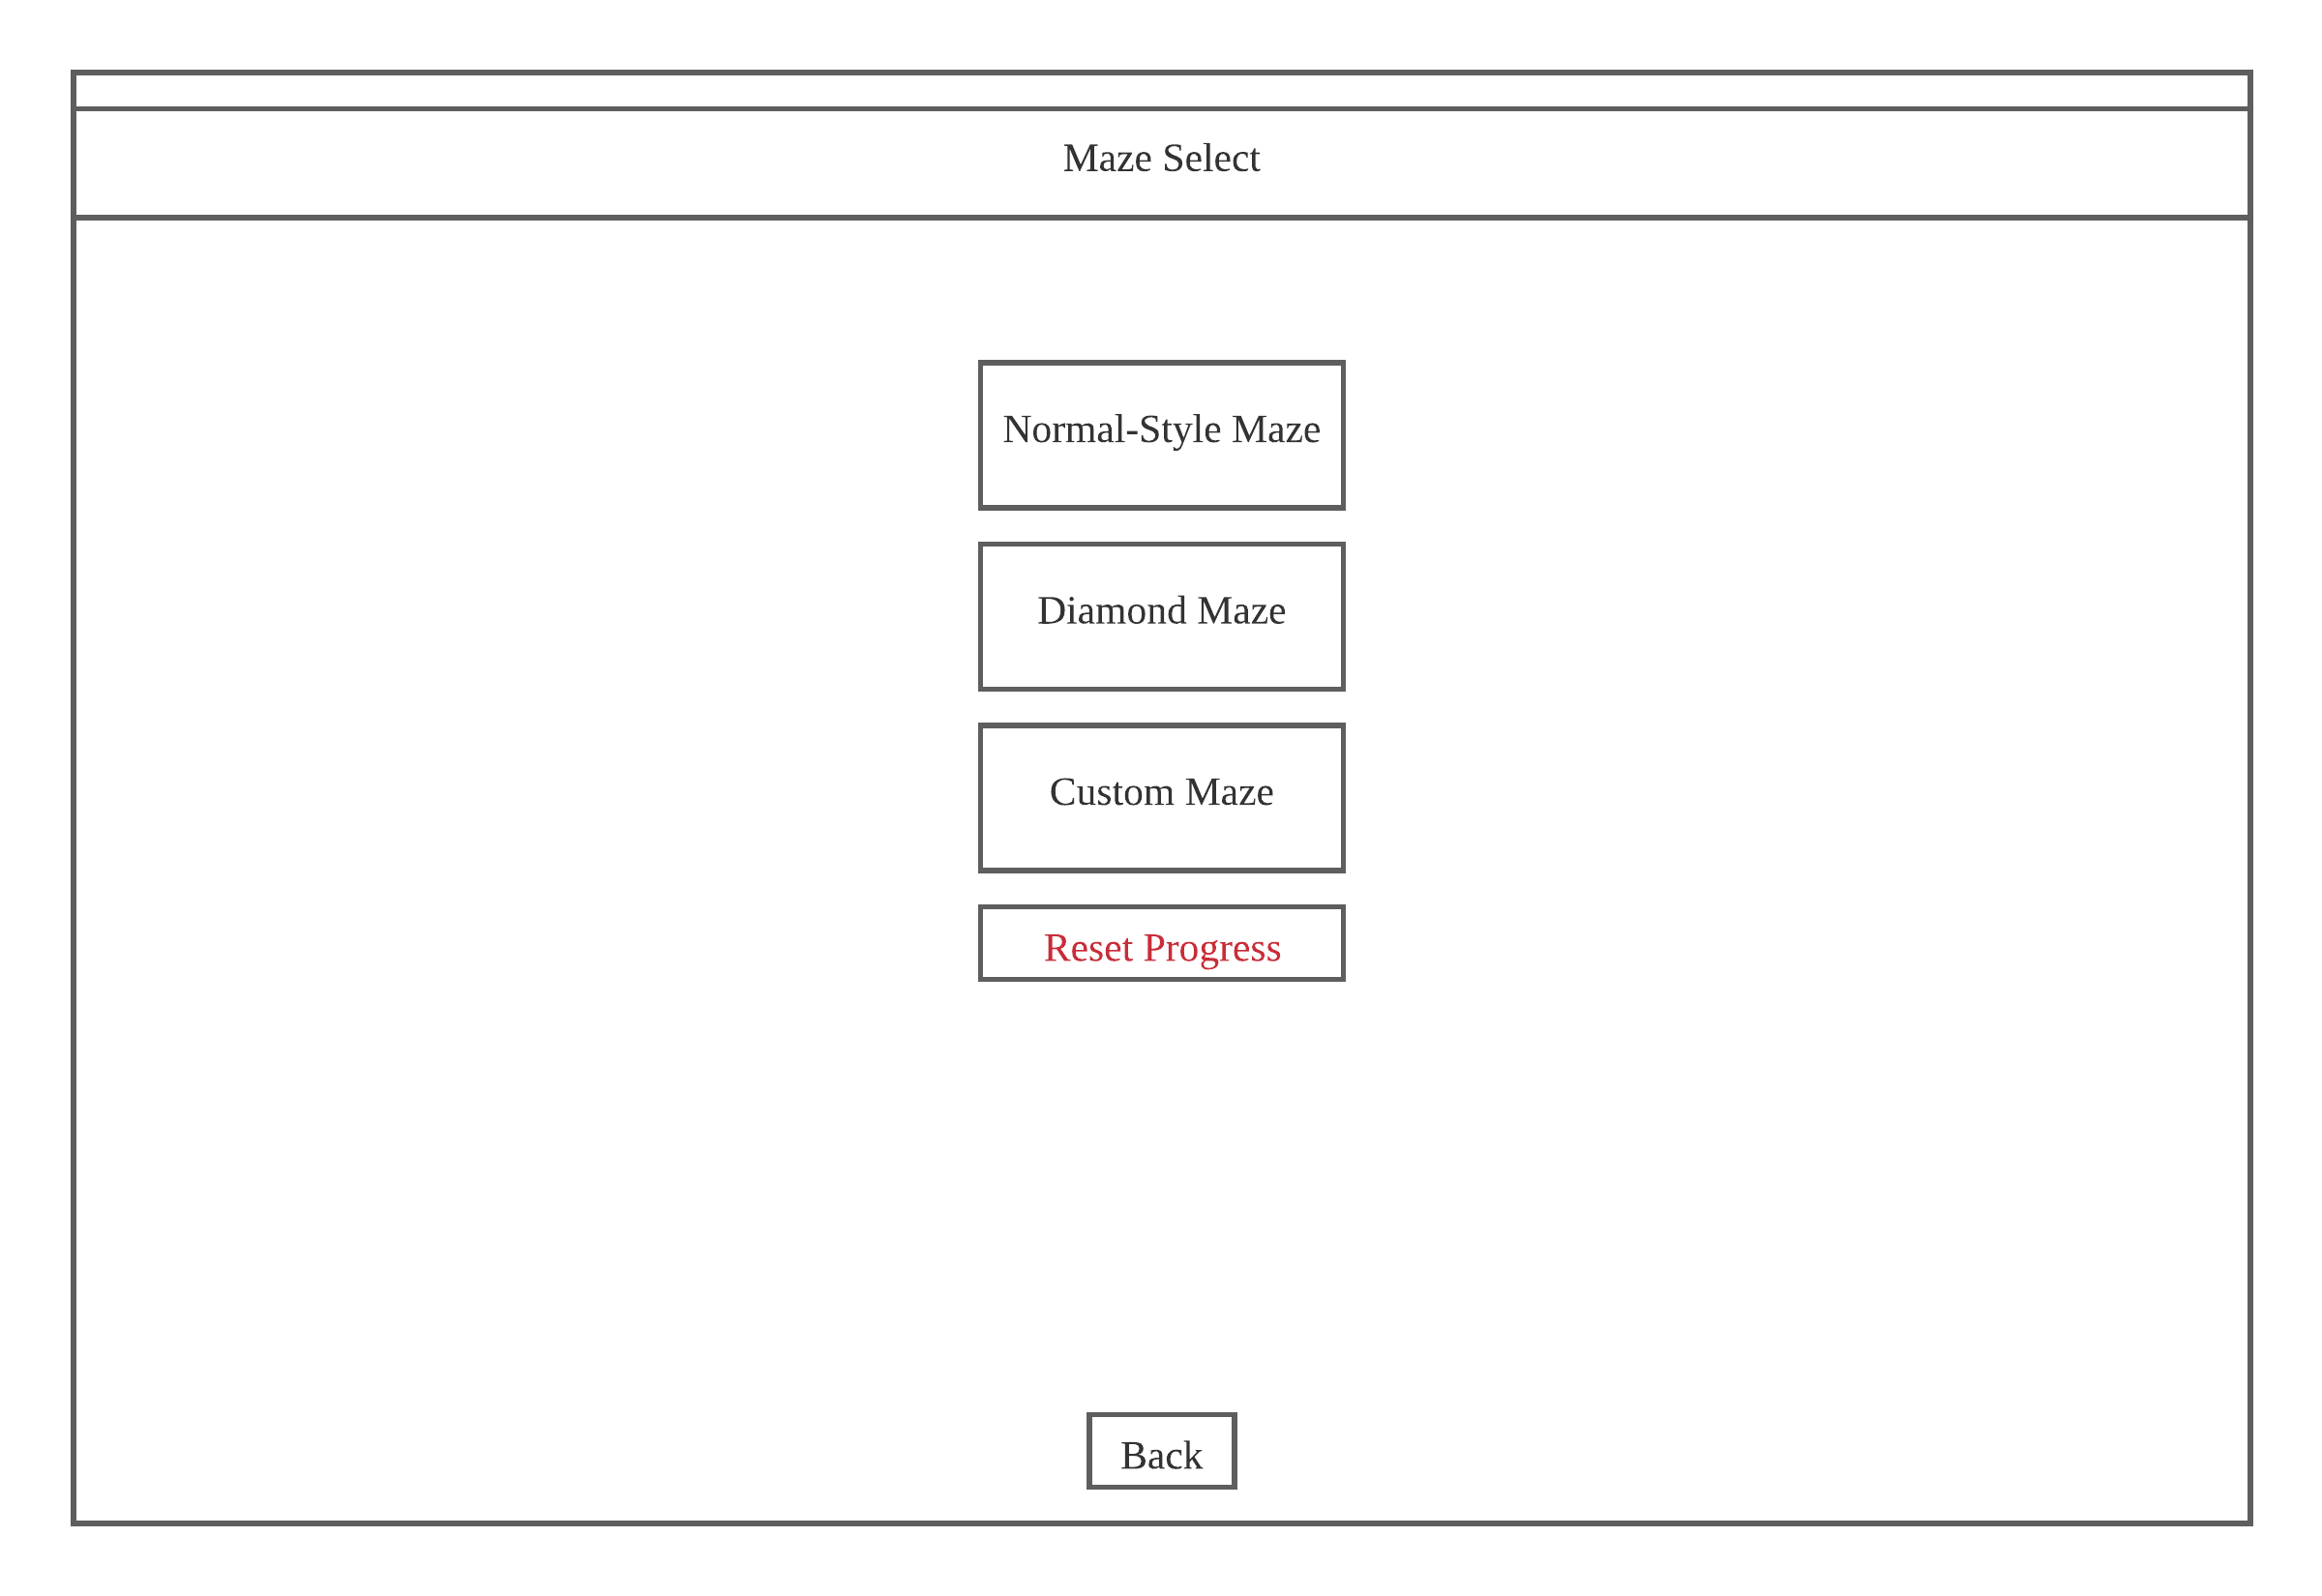
\includegraphics[scale=0.7]{Maze Select Screen}

	On the maze select screen all current maze types are displayed as buttons, in the image above these are; "Normal-Style Maze", "Diamond Maze" and "Custom Maze".
	There is also a "Reset Progress" button that, if the user isn't a guest, will reset their completed levels entry in the maze database. It also has a back button which takes
	the user back to the user select screen.
\end{center}

\clearpage
\begin{center}
%Level Select Screen
	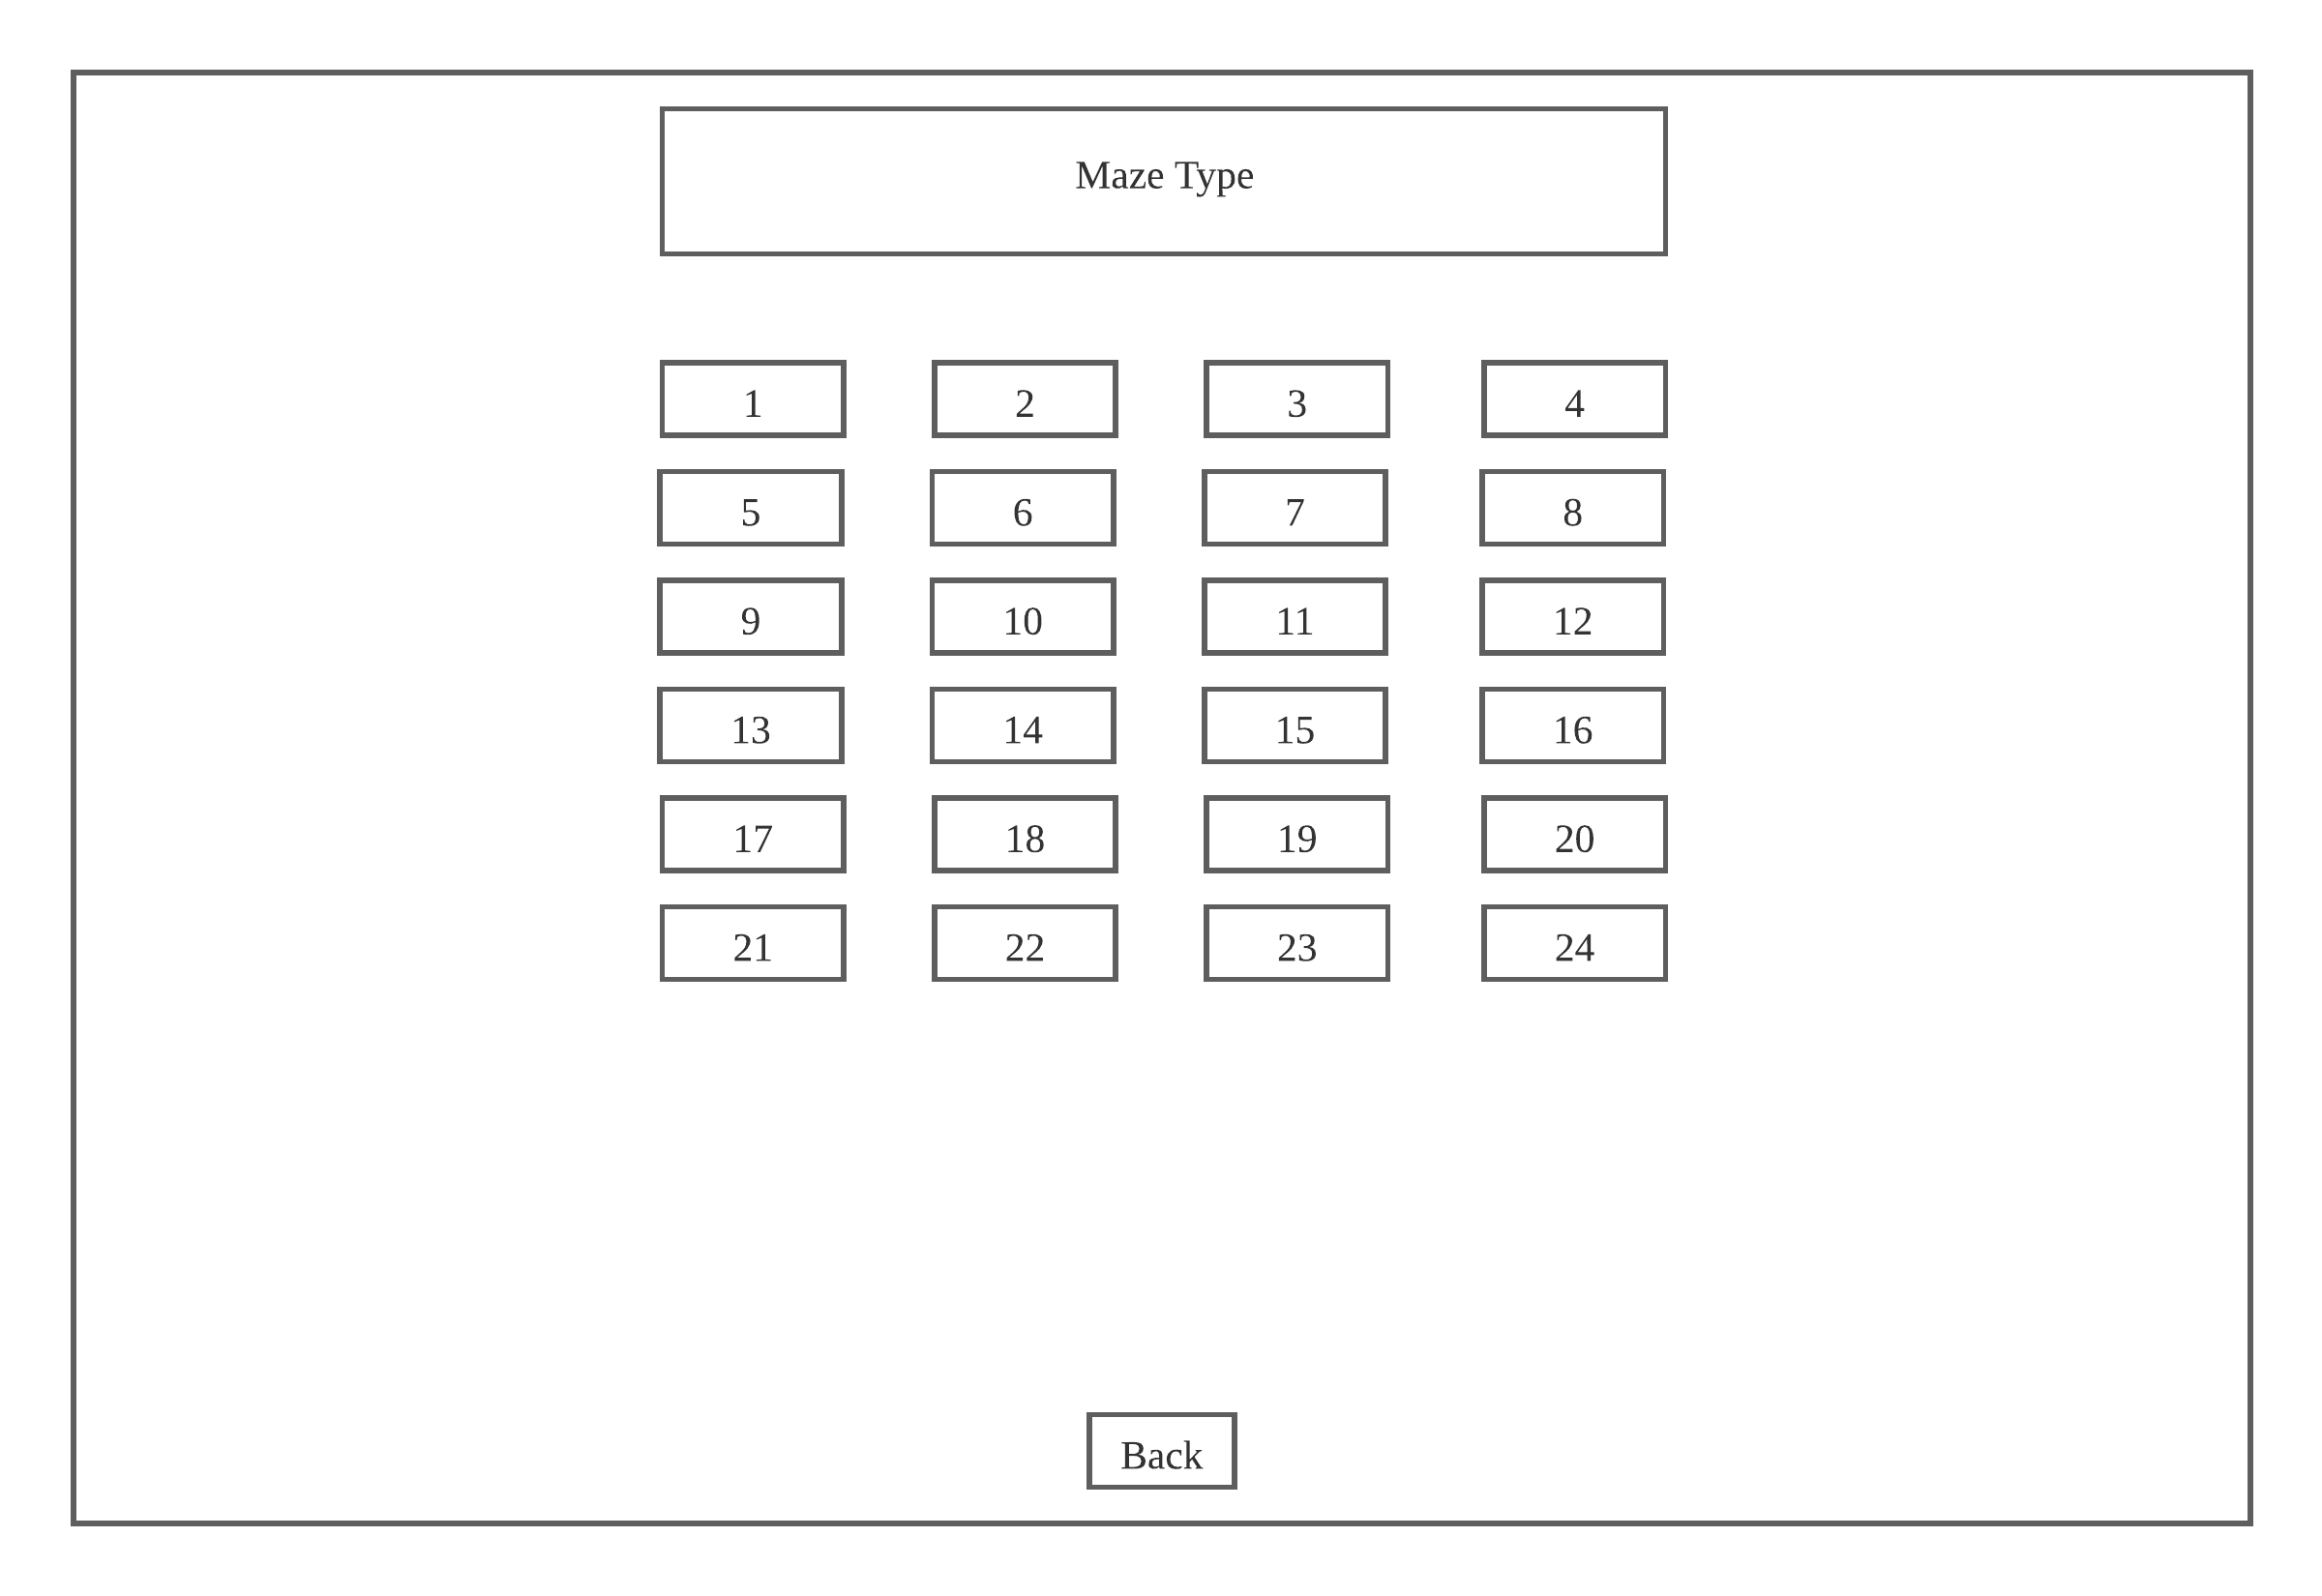
\includegraphics[scale=0.7]{Maze Level Select}

	The maze level select screen consists of rows of buttons that are generated iteratively, each button with a number correlating to the difficulty of the level
	(The actual size of the maze is the number+3). Like the other screens there is a back button, which in this case, leads back to the maze type select screen.
\end{center}
\begin{center}
%Custom Maze Screen
	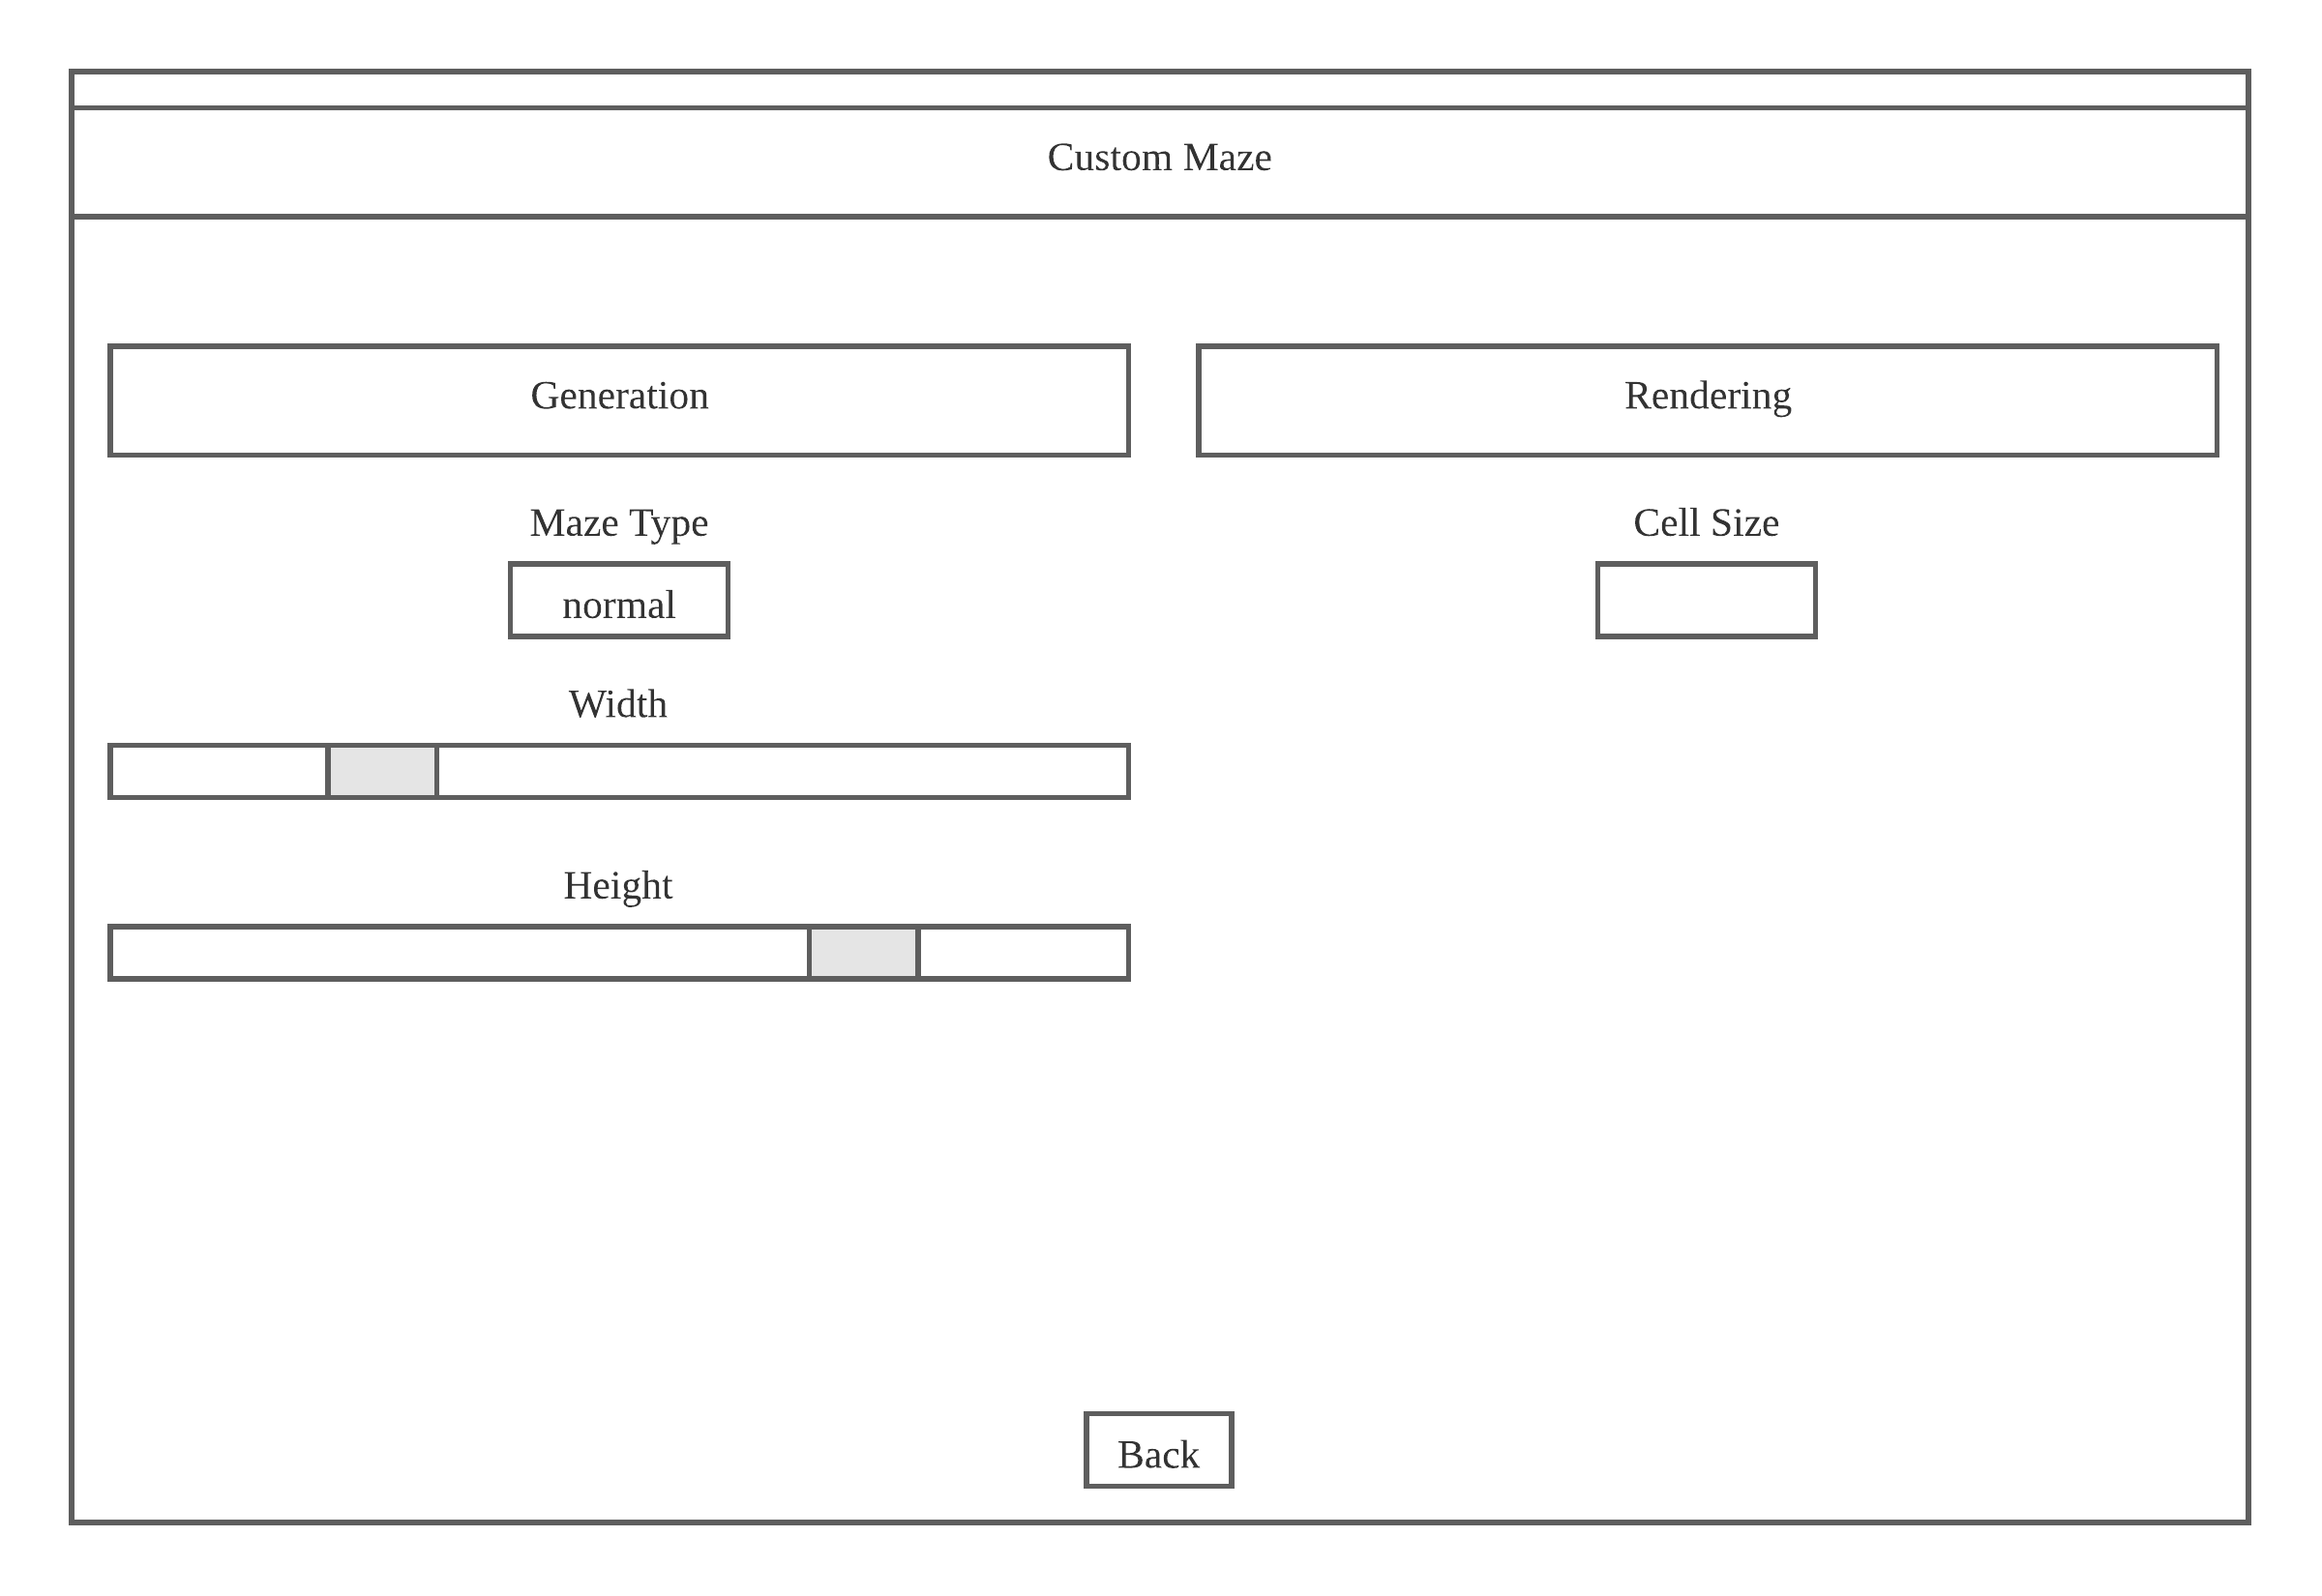
\includegraphics[scale=0.7]{Custom Maze Screen}

	Included on the custom maze screen is halves, one dedicated to rendering and the other to generation. The generation options are maze type, width
	and height, while the only option for rendering is cell size. More options could certainly be added (as my rendering scripts allow for it) if I had more time.
\end{center}
\clearpage
\subsection{Game Visuals}
\begin{center}
%Loading Screen
	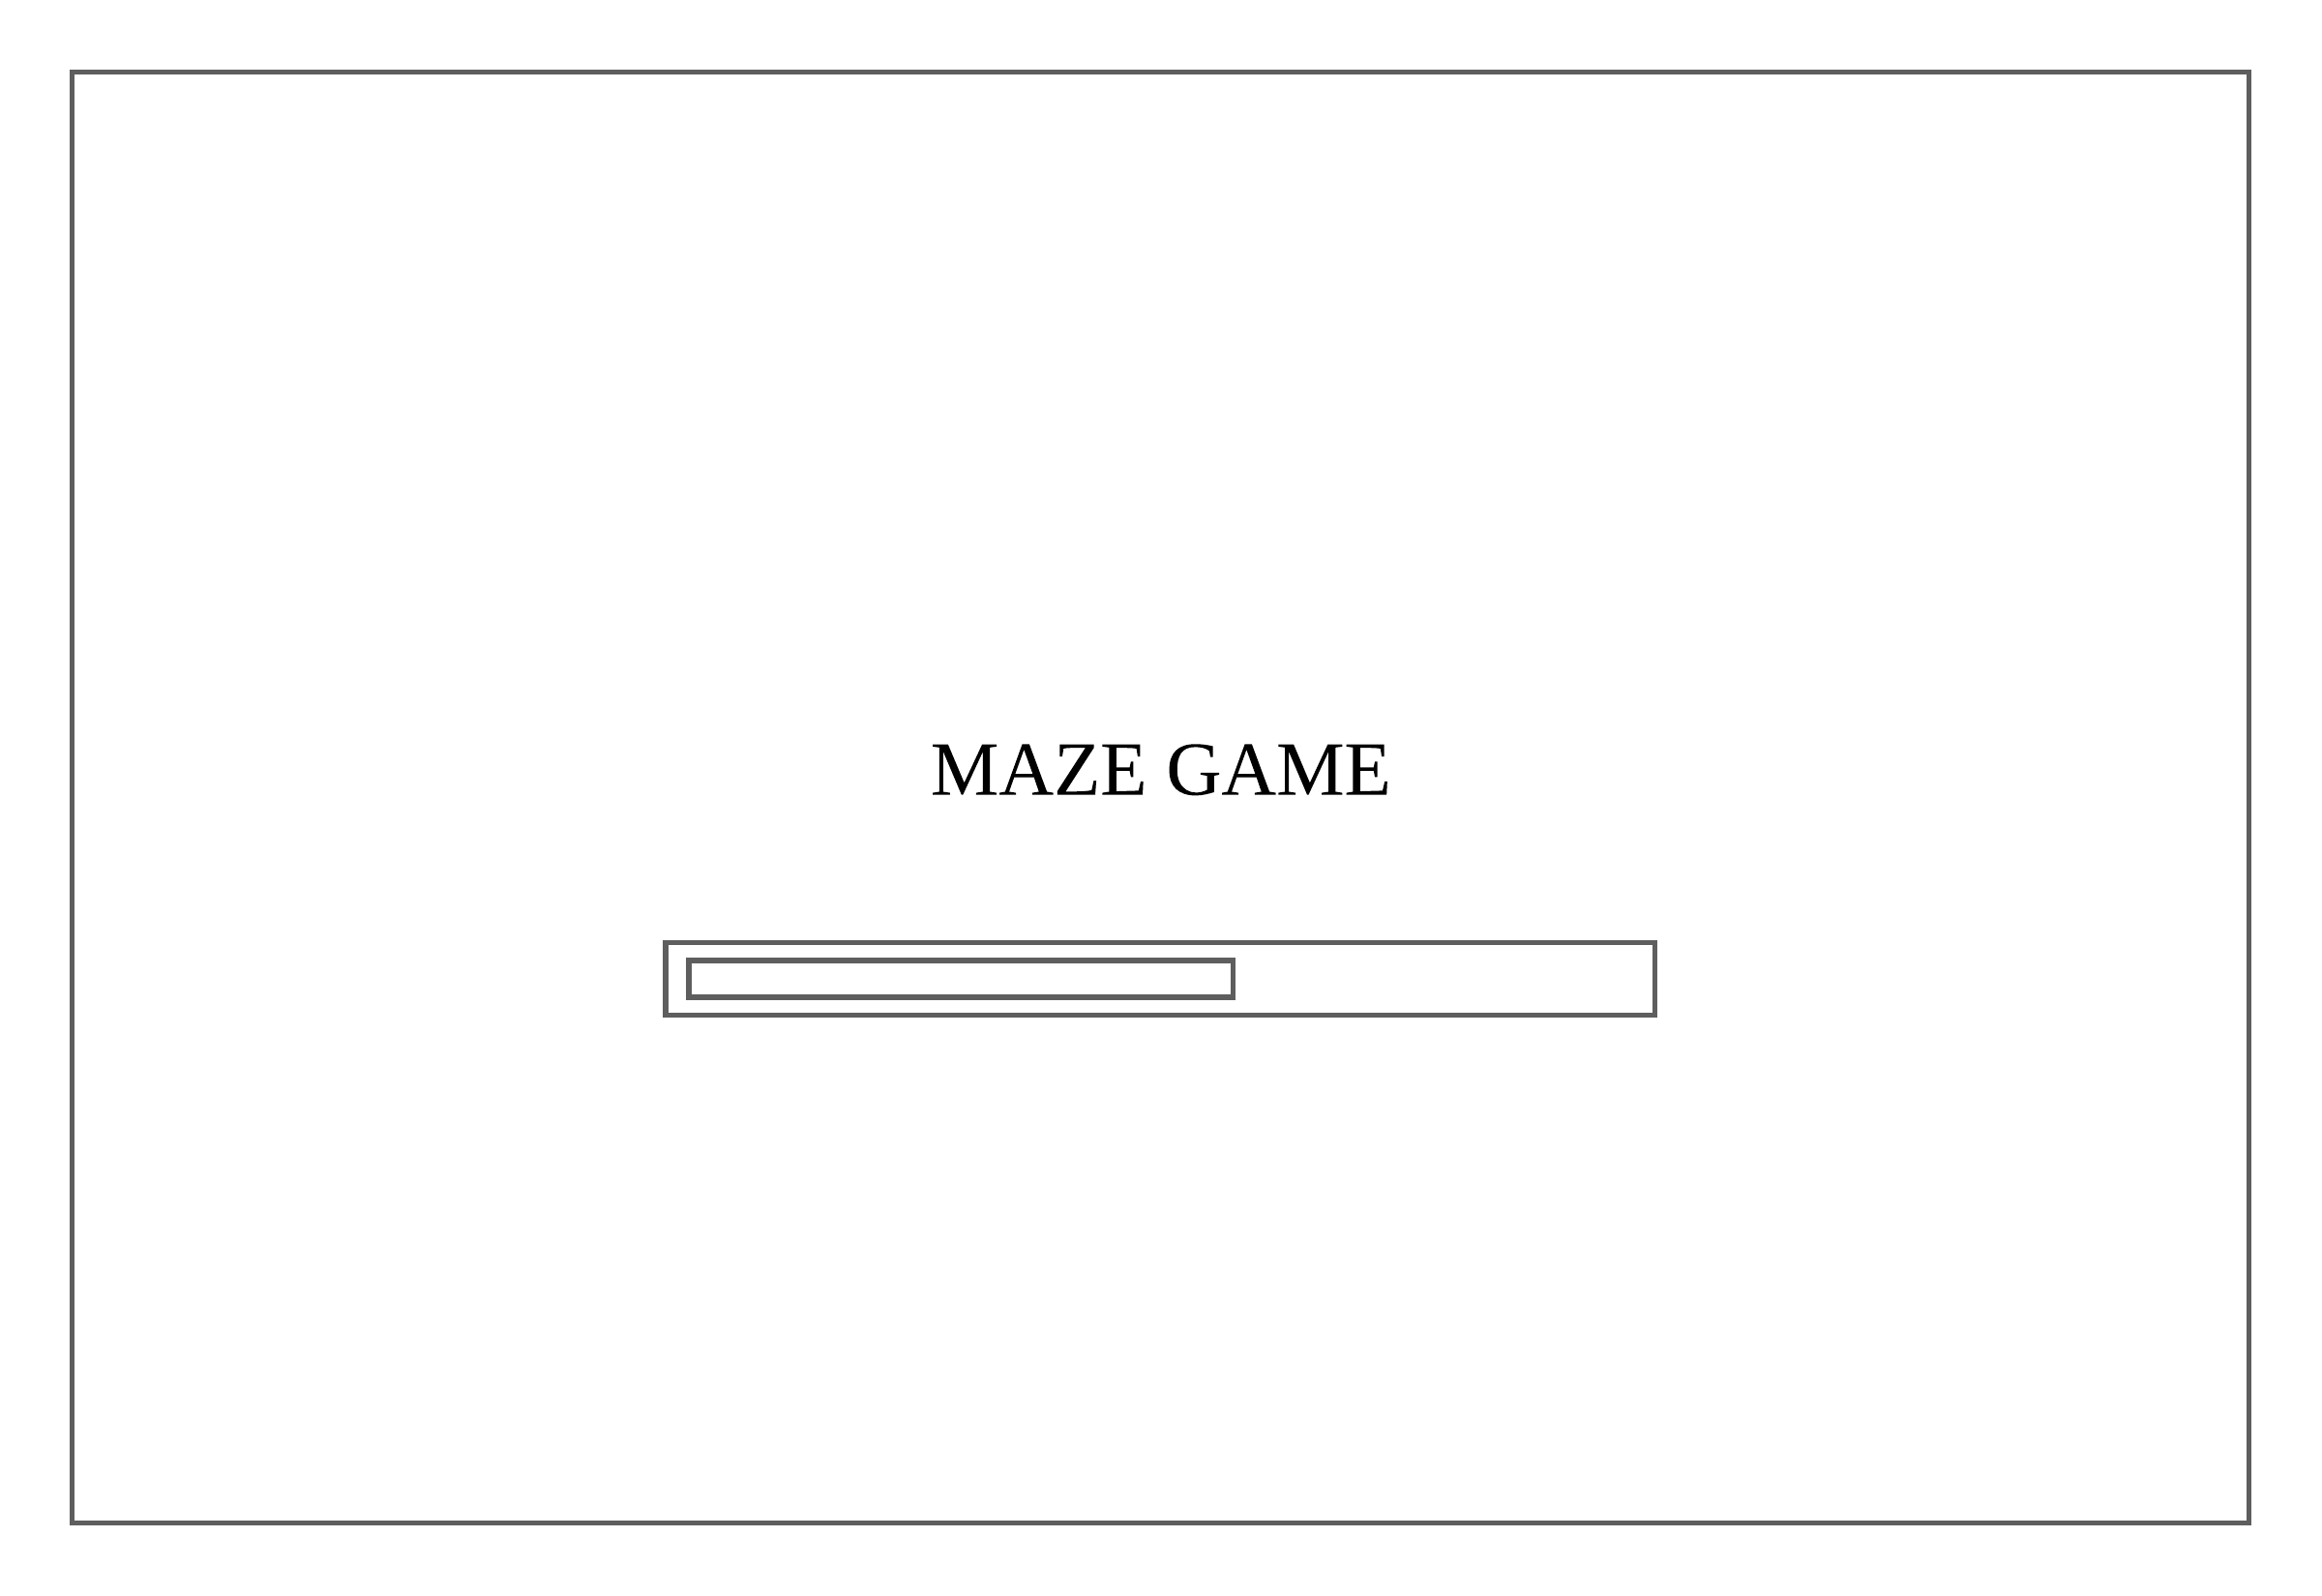
\includegraphics[scale=0.7]{Loading Screen}
	
	Above is the loading/title screen meant to create a slight delay between the level select screen and playing the actual maze, mainly to give the game
	a nicer feel. In actuality the loading bar isn't actual linked to any loading, though if I had more time, through the use of a recursive function, I could pair it with
	the maze generation.
\end{center}
\begin{center}
%Maze Screen
	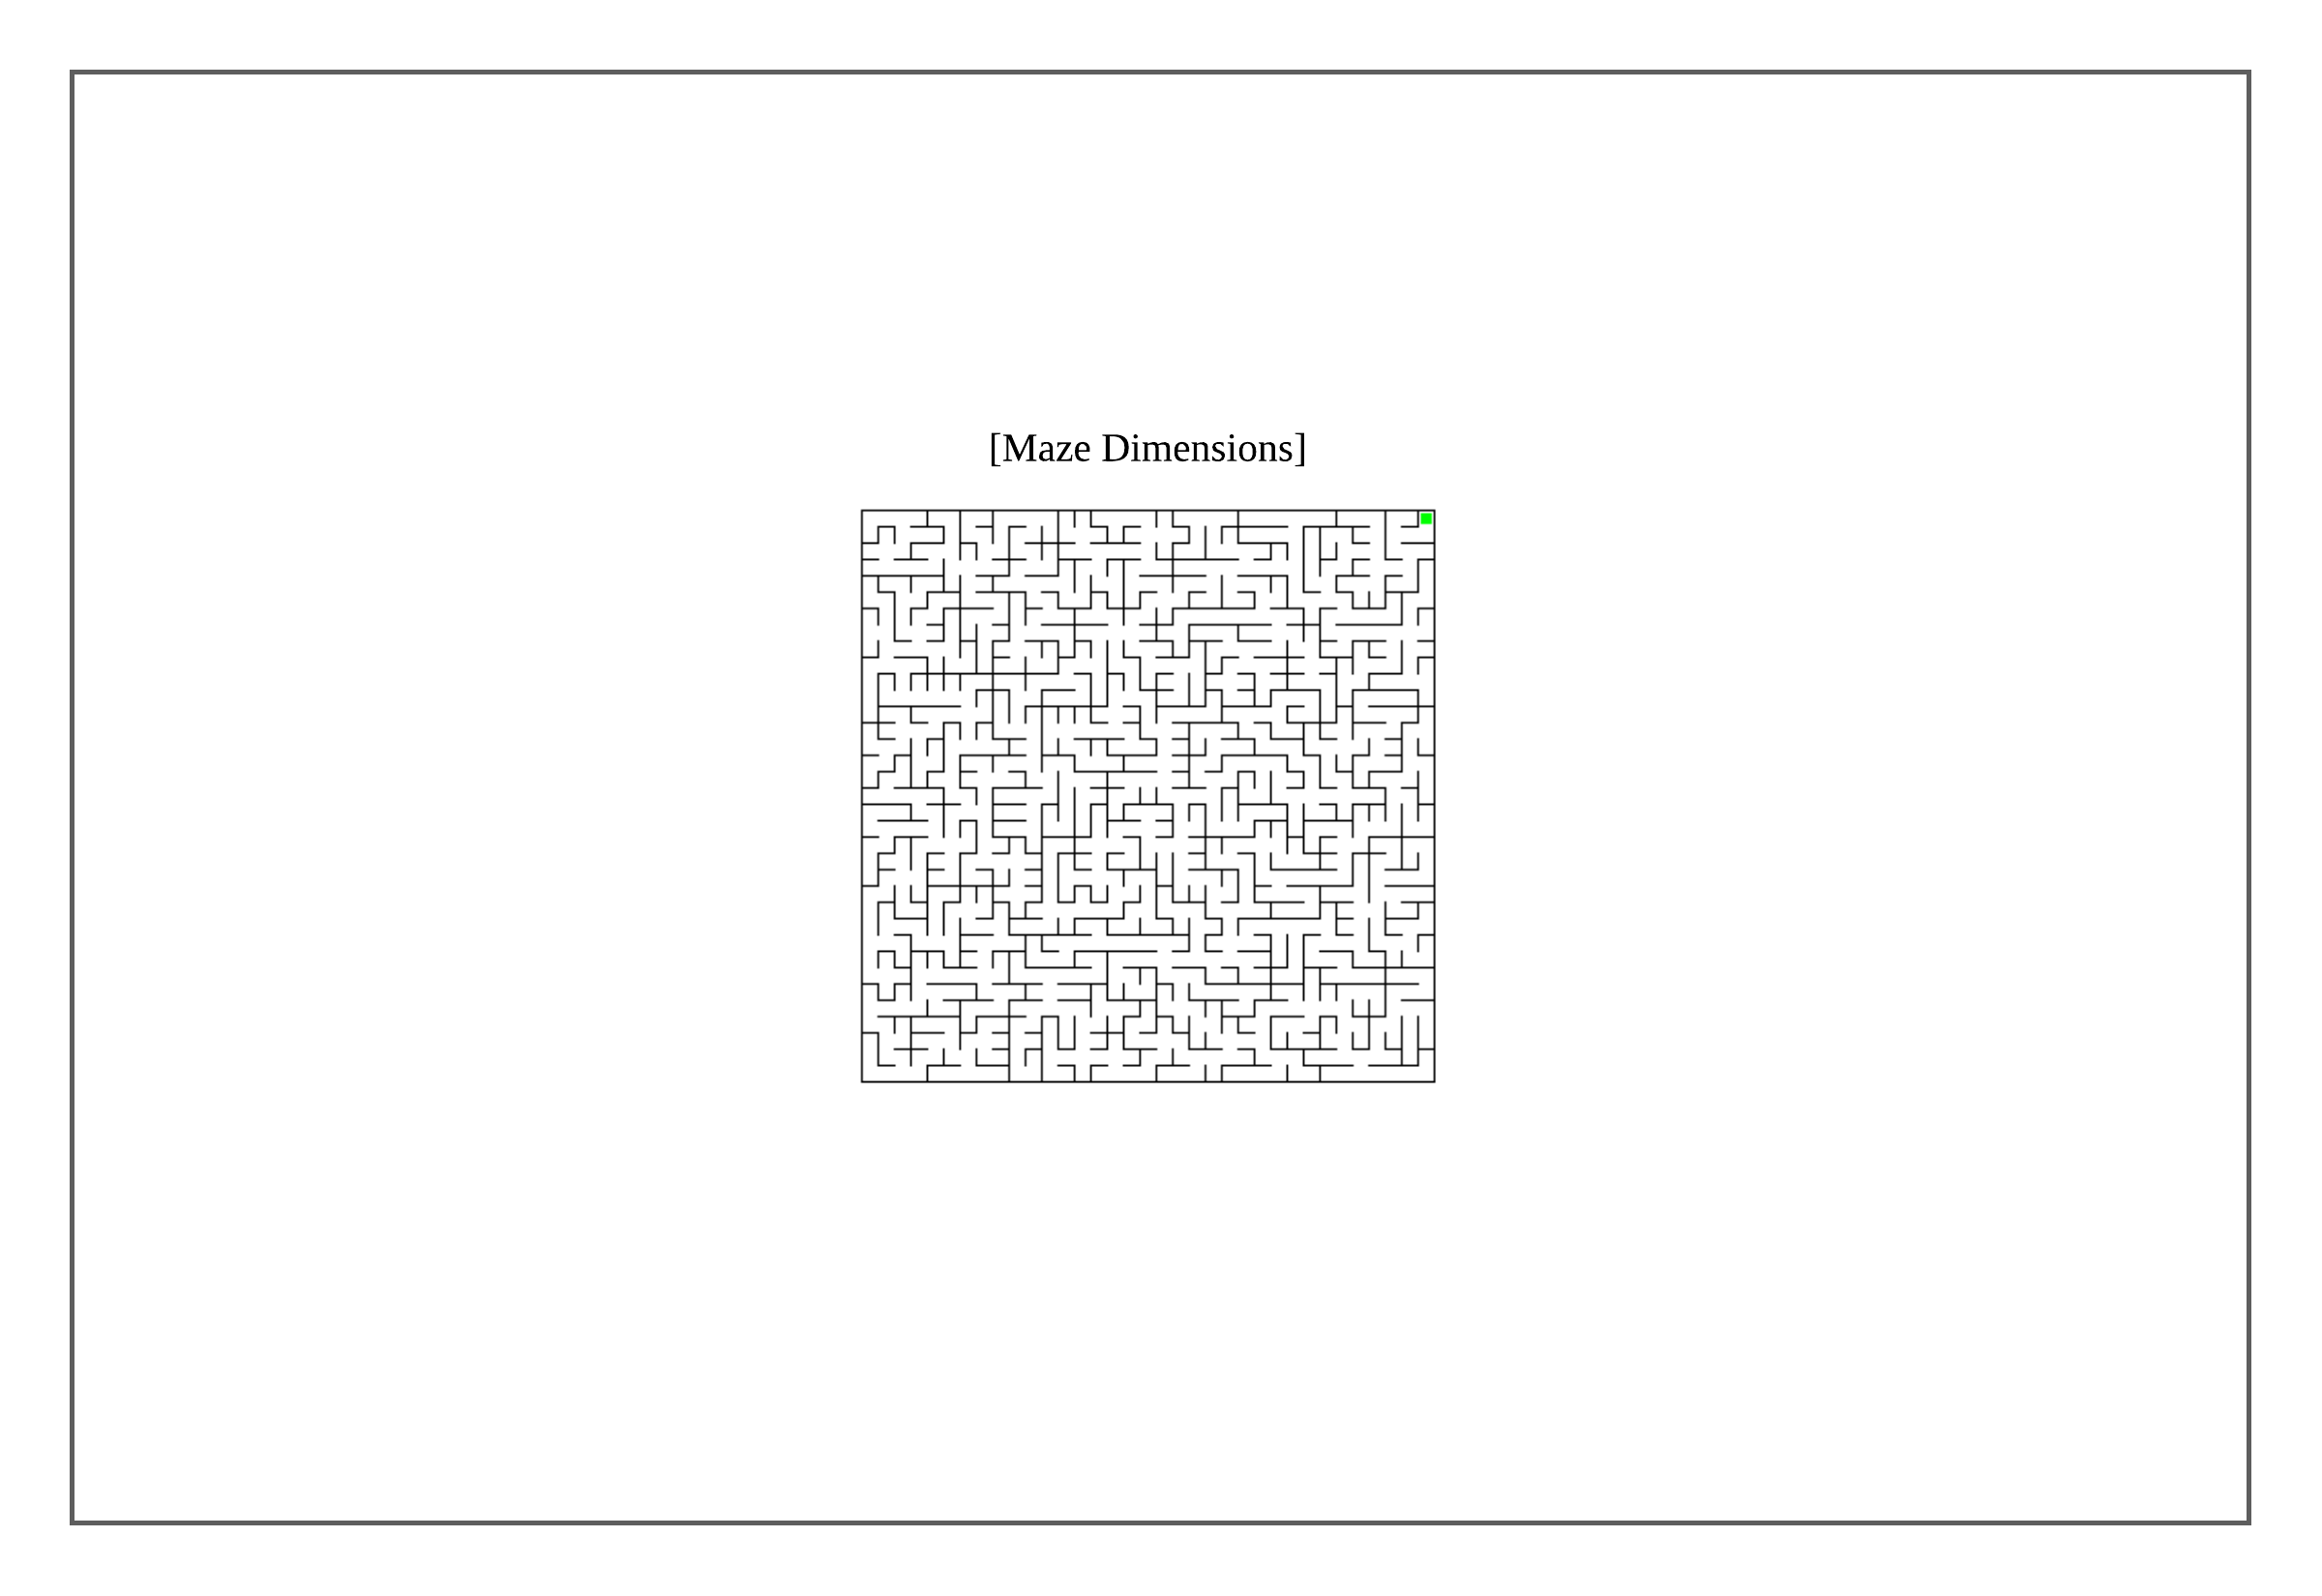
\includegraphics[scale=0.7]{Maze Screen}

	The screen above is where the actual maze will be played, with an example 35 by 35 maze shown.  Above the maze proper is the maze dimensions,
	serving as a title.
\end{center}
\clearpage
\begin{center}
%Maze Completed Screen
	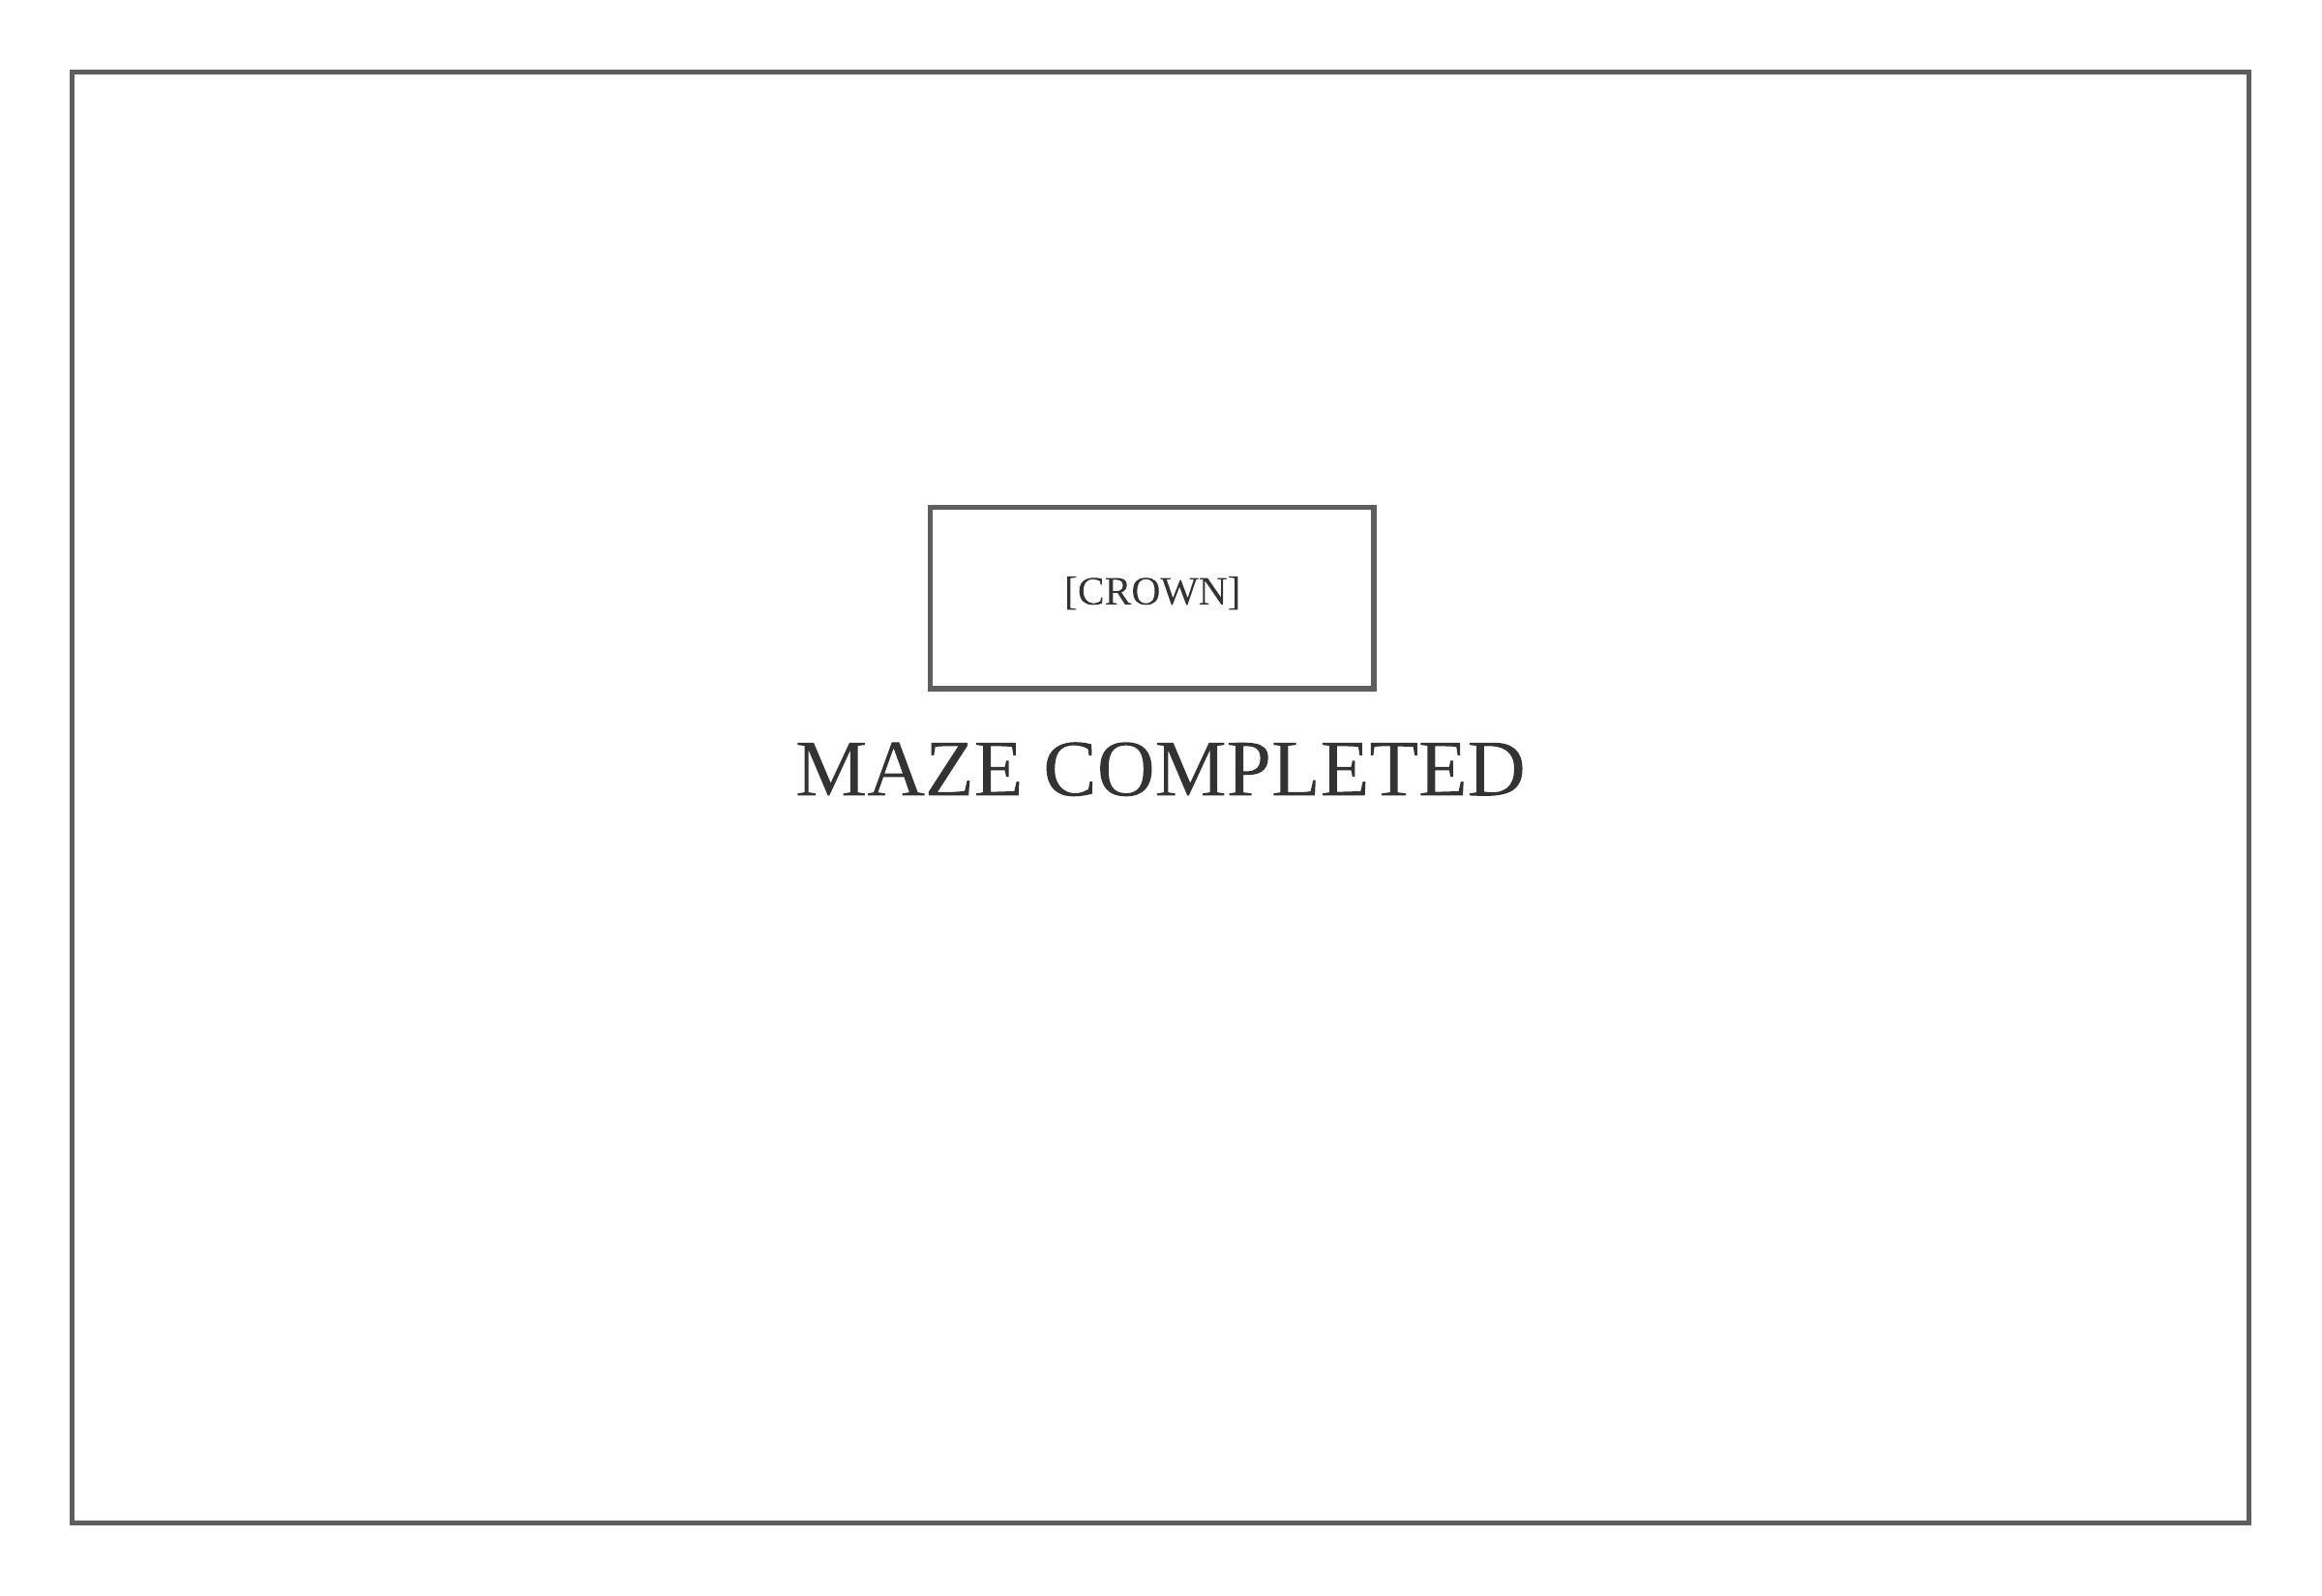
\includegraphics[scale=0.7]{Maze Completed}

	This screen is displayed for a few seconds after the maze is completed, it features the words "Maze Completed" along with a little pixel art crown.
\end{center}

%%%%%%%%%%%%%%%%%%%%%%%%%%


\clearpage
\part{Full Code breakdown by Function}
\section{main.py}
This script handles the creation of the UI as well as running the Maze Database, MazeGenerationNew and 
MazeRendererNew scripts.

\textcolor[RGB]{220,220,220}{\rule{\linewidth}{0.2pt}}
\begin{lstlisting}
def change_state(state):      

    des()
    if state == "start":    
        title = tk.Label(window, text = "\n Maze Game \n Version 2.0 \n", bg = "white", borderwidth=1, relief="groove").pack(fill = "x",pady=(250,20))
        enter_button = tk.Button(window, text = "Enter",bg = "white",width=30, command = lambda: change_state("username")).pack()
        exit_button = tk.Button(window, text = "Exit",width=30, bg = "white", fg = "red", command = lambda: exit()).pack(pady=3)
        if not installed:
            error_message = tk.Label(window,text="[PIL or Numpy not installed, PIL and Numpy are required for current version]",fg="red").pack(side="bottom",pady = 20)
    if state == "username": 
        title = tk.Label(window, text = "\n Accounts \n", bg = "white",  borderwidth=1, relief="groove").pack(fill = "x",pady=(20,100))
        top_seperator = tk.Canvas(window, height=50,width=0).pack()
        ...
\end{lstlisting}
The "change state" function takes the argument "state" and uses that to switch to a pre-defined set of UI elements, e.g. a main menu or a user select screen.

\begin{lstlisting}
def create_levels(lower,upper,number_of_columns,title,maze_type,completed):
    des()
    first = tk.Frame(window)
    first.pack(side='top')
    side = first
    title_ = tk.Label(window, text = ("\n" + title + "\nSelect a level\n"), bg = "white", borderwidth = 1, relief = "groove").pack(in_ = first,fill = "x",pady=20)
    top_seperator = tk.Canvas(window, height=50,width=0).pack(in_ = side)
    dict_one = {
                "normal":0,
                "diamond":1
                }
    for i in range((lower),(upper+1)):
            text = str(i)                          
            try:
                if completed[dict_one[maze_type]].count(text) > 0:
                    fg = "green"
                    text += "\n(Complete)"
                else:
                    fg = "black"
            except:
                fg = "black"
            button = tk.Button(window, text=text, width = 10, relief = 'groove', bg = "white",fg = fg)
            button.config(command = lambda mt = maze_type, btn = button : load_maze(lower,upper,title,mt,dict_one[maze_type],btn))
            button.pack(in_ = side, side = "left", padx=10,pady=10)
            if (i%number_of_columns) == 0:
                middle = tk.Frame(window)
                middle.pack(side = "top")
                side = middle
    back_button = tk.Button(window, text = "Back", command = lambda: change_state("maze select")).pack(side="bottom",pady=10)

\end{lstlisting}
"Create levels" generates a set of buttons with numbers on them, defined by the range entered in the parameters (lower and upper). If the level has already been completed by the user then the text will be green! It lays them out based on the parameter "number\_of\_columns".
When the user clicks on one of these buttons the actual button is passed to the function so that the text on the button can be properly read.

\clearpage

\begin{lstlisting}
def load_maze(lower,upper,title,maze_type,btn):   #Generates the maze and then passes the data along with other parameters to the MazeRenderer script
    maze_size = int((btn['text']).replace("\n(Complete)","")) + 3
    if installed:        
        maze_data = main(maze_size,maze_size,1000,maze_type)
        dict_two = {
            "normal":[[len(maze_data[0])-1],[0],[0,len(maze_data)-1]],
            "diamond":[[len(maze_data[0])-1],[0],[0,len(maze_data)-1]]
            }
        win_pos_x = (dict_two[maze_type])[0]
        win_pos_y = (dict_two[maze_type])[1]
        start_pos = (dict_two[maze_type])[2]
        dimensions = alter_screen()
        won = play_maze(dimensions[0],dimensions[1],(str(maze_size) + " x " + str(maze_size)),10,win_pos_x,win_pos_y,start_pos,maze_data)
    else:
        won = True  #Maze auto-completes if PIL is not installed
    if won:
        if user_id != 0:
            Db.add_completed_level(connection,maze_size-3, maze_type,user_id)
    completed = Db.get_list_of_completed_levels(connection,user_id)
    create_levels(lower,upper,4,title,maze_type,completed)

\end{lstlisting}
The main job of "Load Maze" is to translate the parameters entered pass them to the MazeGenerationNew, script take the generated
data and then pass that, along with other translated parameters, to the MazeRenderNew script.

\begin{lstlisting}
def custom_maze(maze_type,width,height,cube_size,title):    #Same as the function above but for custom mazes
        width = int(width.get())
        height = int(height.get())
        cube_size = int(cube_size.get())
        maze_data = main(width,height,1000,maze_type.get())
        dimensions = alter_screen()
        play_maze(dimensions[0],dimensions[1],(str(width) + " x " + str(height)),cube_size,[len(maze_data[0])-1],[0],[0,len(maze_data)-1],maze_data)
        change_state('custom maze',True)

\end{lstlisting}
"Custom Maze" is a version of "Load Maze" for cutom mazes with unsual heights and widths. An improvement to the code would be combining the two above functions.

\begin{lstlisting}
def set_user_id(username,guest):    #Sets the user ID
    global user_id
    if guest:
        user_id = 0
    else:
        user_id = username
    change_state("maze select")

\end{lstlisting}
"Set User ID" is a simple function that sets the global user\_id. The user\_id is used to retrieve data about the user from maze.db, if the user is a guest then the ID is set to 0
and all code involving the user\_id is skipped.

\begin{lstlisting}
def reset_progress():           #Resets the current users progress
    username = Db.delete_user(connection, user_id)
    Db.create_new_user(connection, username)
    change_state("maze select")
\end{lstlisting}
This functions is also simple. It resets the progress of the user by deleting the user from the and then creating them again, utilizing the below function.

\begin{lstlisting}
def new_user(user_entry_widget):    #Creates a new user named using the entered user name
    name = user_entry_widget.get()
    Db.create_new_user(connection,name)
    change_state("username")
\end{lstlisting}
Simply, adds a new entry to the database containing a new user.

\clearpage

\begin{lstlisting}
def des(): #Deletes all current widgets in "window"
    widget_list = all_children(window)
    for item in widget_list:
        item.pack_forget()
\end{lstlisting}
This function deletes all current widgets, this is used to reset the UI so that new UI can be made in its place. It utilizes the below function
which creates a list of all widgets pareneted to the entered object. The object entered in the case of "des()"  is the whole tkinter window.
\begin{lstlisting}
def all_children(window): # This makes a list of all the current widgets
    list_one = window.winfo_children()
    for item in list_one:
        if item.winfo_children() :
            list_one.extend(item.winfo_children())
    return list_one
\end{lstlisting}

\begin{lstlisting}
def alter_screen():     #Changes screen dimenions to make the rendering of the maze faster
    const = 2
    dimensions = [0,0]
    dimensions[0] = int(screen_width/const)
    dimensions[1] = int(screen_height/const)
    return dimensions
\end{lstlisting}
"Alter Screen" shrinks the size of the layers (images created in the renderer) to make the creation of said layers in the rendering section of the code easier
and less resource consuming.

%%%%%%%%%%%%%%%%%%%%%%%%%%

\clearpage
\section{MazeDatabase.py}
Script for interaction with the maze.db for storing users and completed levels, utilizes SQL.

\textcolor[RGB]{220,220,220}{\rule{\linewidth}{0.2pt}}
\begin{lstlisting}
def main_database():    #Creates the database (if it wasn't already created) and establishes a connection to it 
    user_table = " CREATE TABLE IF NOT EXISTS users (
id integer PRIMARY KEY,
username text NOT NULL
); "
    completed_levels_table = " CREATE TABLE IF NOT EXISTS completedLevels (
id integer PRIMARY KEY,
normal_maze text,
diamond_maze text,
user_id integer NOT NULL,
FOREIGN KEY (user_id) REFERENCES users (id)
); " 
    connection = create_connection(r"Maze.db")
    if connection is not None:
        create_table(connection,user_table)
        create_table(connection,completed_levels_table)
    else:
        print("Database Connection Error")
    return connection
\end{lstlisting}
This function is run to intialize the database, composed of two tables, (if it's not already created) and  establish a connection to said database.
The comment explaining the datbase is included below, along with a diagram.
\begin{lstlisting}
"DATABASES
Users table stores name and user_id + any additional information needed
CompletedLevels table stores the completed levels linked to the foreign key user_id and a primary key completed_id. There will be two columns, one for normal mazes, one for diamond mazes
the completed levels will be serialized as such (1#3#4#12...) and when the string is imported it will be split into a list."
\end{lstlisting}
\begin{center}
	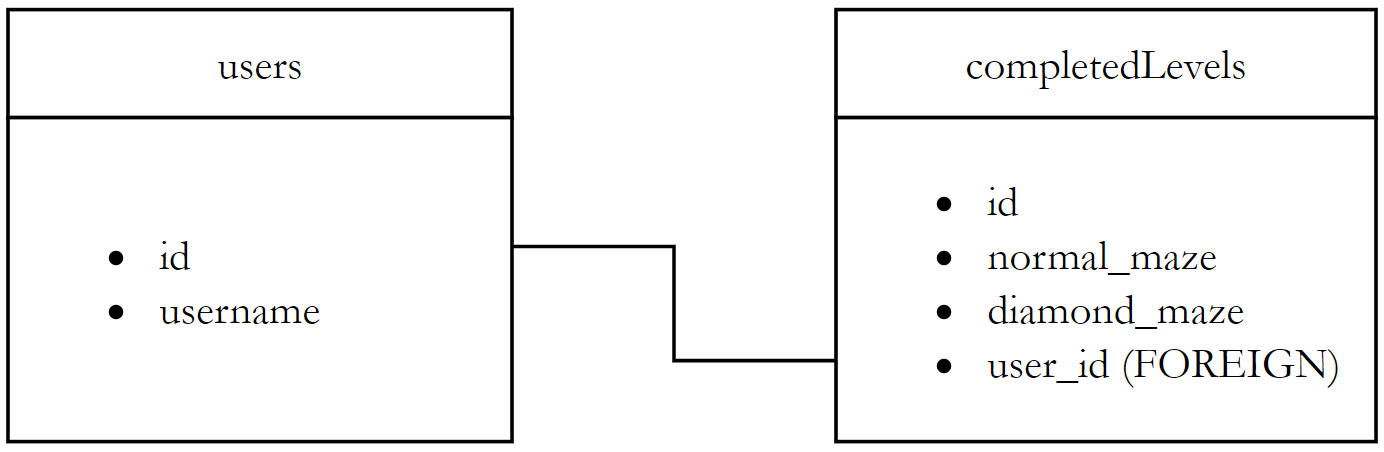
\includegraphics[scale=0.5]{Database Diagram}
\end{center}
\begin{lstlisting}
def create_new_user(connection, username):
    #Create the new user
    new_user_sql = "INSERT INTO users(username) VALUES(?)"
    cursor = connection.cursor()
    cursor.execute(new_user_sql, (username,))
    user_id = cursor.lastrowid
    connection.commit()
    #Then create the sibling entry in the CompletedLevels table based of the generated user_id
    new_completed_levels_sql = "INSERT INTO completedLevels(normal_maze, diamond_maze, user_id) VALUES(?,?,?)"
    cursor = connection.cursor()
    cursor.execute(new_completed_levels_sql, ("","",user_id))
    connection.commit()
\end{lstlisting}
"Create New User" inserts a row into the \textbf{users} table containing the entered username and then makes a sister entry in \textbf{completedLevels}. It uses
cursor.lastrowid to get the correct user id.
\clearpage
\begin{lstlisting}
def delete_user(connection, user_id):
    sql = 'SELECT username FROM users WHERE id = ?'
    cursor = connection.cursor()
    cursor.execute(sql, (user_id))
    result = cursor.fetchall()
    #Delete user entry
    sql = 'DELETE FROM users WHERE id=?'
    cursor = connection.cursor()
    cursor.execute(sql, (user_id))
    connection.commit()
    #Delete completedLevels entry
    sql = 'DELETE FROM completedLevels WHERE user_id=?'
    cursor = connection.cursor()
    cursor.execute(sql, (user_id))
    connection.commit()
    return result[0][0]
\end{lstlisting}
"Delete User" removes an entry from users and completedLevels based on the entered user\_id. It will also return the username from said user so that they can
be recreated in the "Reset Progress" function.

\begin{lstlisting}
def get_list_of_users(connection):
    user_list = []
    cursor = connection.cursor()
    cursor.execute("SELECT * FROM users")
    result = cursor.fetchall()
    for row in result:
        user_list.append((str(row)[1:-1]).split(','))
    return user_list
\end{lstlisting}
This function is implemented in "Change State" and is used when creating the buttons for the users in the user select screen. Contained within each
entry in the list is both the user\_id and the username.

\begin{lstlisting}
def add_completed_level(connection, level_number, maze_type, user_id):    #Uses the user id to alter the user's completed levels
    completed = get_list_of_completed_levels(connection, user_id)
    dict_one = {
                "normal":0,
                "diamond":1
                }
    formatted = ''
    for level_num in completed[dict_one[maze_type]]:
        print(level_num)
        formatted = formatted + level_num + "#"
    formatted = formatted + str(level_number)
    if maze_type == "normal":
        sql = "UPDATE completedLevels SET normal_maze = ? WHERE user_id = ?"
    elif maze_type == "diamond":
        sql = "UPDATE completedLevels SET diamond_maze = ? WHERE user_id = ?"
    cursor = connection.cursor()
    cursor.execute(sql,(formatted,user_id))
\end{lstlisting}
"Add Completed Level" takes the current completed levels list converts it to a string,  adds the entered level to the string and then inserts
it into the correct entry in the database. It finds the correct entry based off the maze type and user\_id.
\begin{lstlisting}
\end{lstlisting}
The below function is implemented in "Add Completed Level" to get the current completed levels for both maze types.
\begin{lstlisting}
def get_list_of_completed_levels(connection, user_id):
    maze_find_sql = "SELECT normal_maze, diamond_maze FROM completedLevels WHERE user_id = ?"
    cursor = connection.cursor()
    cursor.execute(maze_find_sql,(user_id))
    result = cursor.fetchall()
    return [(result[0][0]).split('#'),(result[0][1]).split('#')]
\end{lstlisting}
"Get List of Completed Levels" takes the string stored in the database for all maze types and converts them into a 2D array. 
The format for the string is explained in the comment explaning the database above.

\clearpage
\begin{lstlisting}
def create_connection(db_file):
    connection = None
    try:
        connection = sqlite3.connect(db_file)
    except Error as e:
        print(e)
    return connection
\end{lstlisting}

\begin{lstlisting}
def create_table(connection, create_table):
    try:
        cursor = connection.cursor()
        cursor.execute(create_table)
    except Error as e:
        print(e)
\end{lstlisting}
The above two functions are standard functions for interacting with a database. "Create Conncetion" creates a connection with a database file or creates the
database file and the establishes a connection with it if it doesn't already exist. The connection is then used the interact with the database itself. "Create Table"
actually would execute any SQL passed to it and acts more like an alias/simplification, however, it is only ever used to create tables.

%%%%%%%%%%%%%%%%%%%%%%%%%%

\clearpage
\section{MazeGenerationNew.py}
Uses Kruskal’s algorithm paired with a generated weight array to create the maze.

\textcolor[RGB]{220,220,220}{\rule{\linewidth}{0.2pt}}
\begin{lstlisting}
def intialize_array(width,height):
    #Intialize the array
    maze_array = []
    for x in range(0,width):
        maze_array.append([])
        for y in range(0,height):
            maze_array[x].append([1,1,1,1]) #Add a blank cell with all four walls to create an array that will be altered to generate a maze, this array is the data we return
    return maze_array
\end{lstlisting}
"Intialize Array" creates a 2D array formatted in the correct manner to be used as the \textbf{maze\_array} which represents the maze. This maze is made
up of cells, each cell being linked to a coordinate/index in the 2D array, with the cell being represented as a list of length four (i.e. [1,1,1,1]). Each number in
this list can be eithier a 1 or 0, representing a wall or empty space respectively. A diagram displaying this is placed below.
\begin{center}
	\fbox{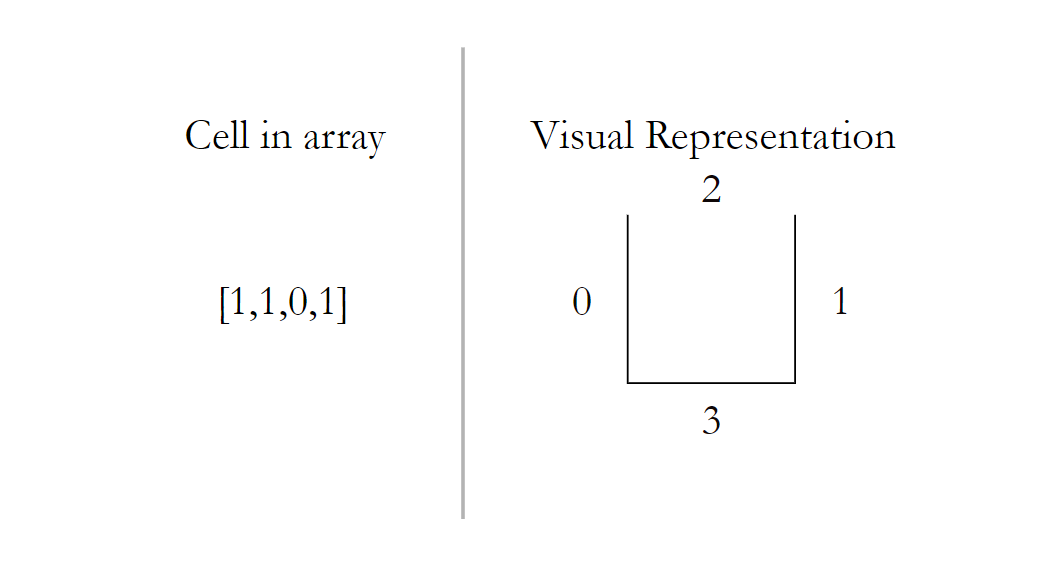
\includegraphics[scale=0.5]{Maze Cell Diagram}}

	\color{mygrey}(The numbers on the Visual Representation correlate to the index in the array)
\end{center}

\begin{lstlisting}
def generate_random_walls(height,width):    #Random walls for testing maze renderer
    #Intialize the array
    maze_array = []
    temp_list = [0,0,0,0,0,0,1]
    for x in range(0,width):
        maze_array.append([])
        for y in range(0,height):
            maze_array[x].append([random.choice(temp_list),random.choice(temp_list),random.choice(temp_list),random.choice(temp_list)])
    return maze_array
\end{lstlisting}
The above function is used only in testing, it can technically generate unbeatable mazes but due to the weighted chance to generate an empty or 
a wall (represented using temp\_list) it is unlikley. It  was mainly used in rendering testing but was also used when testing maze collision. 
\clearpage
\begin{lstlisting}
def kruskals_algorithim(weight_group_array,width,height,max_weight): #Based loosely on the algorithim as described in "Mazes for Programmers"
    maze_array = intialize_array(width,height)
    group_designation = 1                                                                                                                                           
    temp_list_empty = False
    while not all_in_one_group(weight_group_array,height,width) and not temp_list_empty: #Only ends loop when no new corridors can be checked and all the corriders are in the same group
        temp_list = lowest_values_pos(weight_group_array,width,height,max_weight+1)
        if temp_list == []:
            temp_list_empty = True
        else:
            dict_one = {
                0:[0,-1,1],
                1:[0,1,0],
                2:[-1,0,3],
                3:[1,0,2]
                }
            for pos in temp_list:
                can_connect = True
                difference = dict_one[pos[2]]
                current_pos_group = (weight_group_array[pos[0]][pos[1]])[4]                
                try:
                    if pos[0]+difference[0] == -1 or pos[1]+difference[1] == -1:
                        error = pos[100]
                    connected_pos_group = (weight_group_array[pos[0]+difference[0]][pos[1]+difference[1]])[4]
                    if current_pos_group == 0:
                        if connected_pos_group == 0:
                            (weight_group_array[pos[0]][pos[1]])[4] = group_designation
                            (weight_group_array[pos[0]+difference[0]][pos[1]+difference[1]])[4] = group_designation
                            group_designation += 1
                        else:
                            (weight_group_array[pos[0]][pos[1]])[4] = (weight_group_array[pos[0]+difference[0]][pos[1]+difference[1]])[4]
                    else:
                        if current_pos_group == connected_pos_group:
                            can_connect = False
                        elif connected_pos_group == 0:
                            (weight_group_array[pos[0]+difference[0]][pos[1]+difference[1]])[4] = current_pos_group
                        elif connected_pos_group != 0:
                            group_pos = get_all_in_group(weight_group_array,width,height,connected_pos_group)
                            for pos2 in group_pos:
                                (weight_group_array[pos2[0]][pos2[1]])[4] = current_pos_group
                    if(can_connect):
                        (maze_array[pos[0]][pos[1]])[pos[2]] = 0
                        (maze_array[pos[0]+difference[0]][pos[1]+difference[1]])[difference[2]] = 0
                    (weight_group_array[pos[0]][pos[1]])[pos[2]] = max_weight+2
                    (weight_group_array[pos[0]+difference[0]][pos[1]+difference[1]])[difference[2]] = max_weight+2
                except IndexError:
                    (weight_group_array[pos[0]][pos[1]])[pos[2]] = max_weight+2
                    if (weight_group_array[pos[0]][pos[1]])[4] == 0:
                        (weight_group_array[pos[0]][pos[1]])[4] = group_designation
                        group_designation += 1
    return maze_array
\end{lstlisting}
"Kruskals Algorithim" is the algorithim used to actually generate the mazes. It does this utilizing a \textbf{weight\_group\_array} and by altering
the corridors between cells in the \textbf{maze\_array}. The outline of how it works is this; All cells have a group, at the start this is the default group (i.e. zero).
Any cell within a group is reachable by any other cell in a group (unless it is the default group), they are essentially perfect mazes within the larger maze.
At the start of each iteration of the while loop the code finds corridors (connections between cells) based on the lowest weight, this is done using the afformentioned
\textbf{weight\_group\_array} and the function below.
\clearpage
\begin{lstlisting}
def lowest_values_pos(wg_array,width,height,compared_to):   #Finds all the connections in the maze with the lowest weight value
    temp_list = []
    for x in range(0,width):
        for y in range(0,height):
            for i in range(0,4):
                if wg_array[x][y][i] < compared_to:
                    compared_to = wg_array[x][y][i]
                    temp_list = []
                    temp_list.append([x,y,i])
                elif wg_array[x][y][i] == compared_to:
                    temp_list.append([x,y,i])
    return temp_list
\end{lstlisting}
The actual \textbf{weight\_group\_array} or\textbf{wg\_array}  is generated by functions "Generate Walled Maze" and "Generate Diamond Maze" discussed lower down.
Once a corridor is chosen an actual connection is attempted, a connection will only not be made if, 1. The connection is being made to an area outside the maze or 2. The
connection is being made to a cell that is already in the same group as the chosen cell. The latter of the two fail states exists so that the generation doesn't remove every single wall.
If a connection is made between two cells with non-default but different groups then all cells in the group that doesn't contain the chosen cell are changed to be in the group
with the chosen cell. This process is done using "Get All In Group" (shown below).
\begin{lstlisting}
def get_all_in_group(wg_array,width,height,group):  #Gets the positions of all the cells that have the group specified
    temp_array = []
    for x in range(0,width):
        for y in range(0,height):
            if (wg_array[x][y])[4] == group:
                temp_array.append([x,y])
    return temp_array
\end{lstlisting}
The algorithim will run untill all cells are in the same group (and that group is not the default) meaning any cell within the maze can be reached from any other cell. To check
that all cells are in the same group the function "All In One Group" is used.
\begin{lstlisting}
def all_in_one_group(wg_array,height,width):    #Checks to see if every cell is in a singular group (a.k.a every cell can be reached from any other cell)
    returned = True
    first_group = "null"
    for x in range(0,width):
        for y in range(0,height):
            temp = (wg_array[x][y])[4]
            if first_group == "null":
                first_group = temp
            if temp != first_group or temp == 0:
                returned = False                
    return returned
\end{lstlisting}
\begin{lstlisting}
def generate_walled_maze(width,height,max_weight):
    weight_group_array = []                 
    for x in range(0,width):
        weight_group_array.append([])
        for y in range(0,height):
            weight_group_array[x].append([random.randint(1,max_weight),random.randint(1,max_weight),random.randint(1,max_weight),random.randint(1,max_weight),0])   #Create a "sister" array that stores the weight values and group of each cell
    maze_array = kruskals_algorithim(weight_group_array,width,height,max_weight)    #Use the weight array to generate an actual maze
    return maze_array
\end{lstlisting}
"Generate Walled Maze" generates a simple \textbf{weight\_group\_array} by randomly generating weight values for each cell.
\clearpage
\begin{lstlisting}
def generate_diamond_maze(width,height,max_weight):
    weight_group_array = []
    for x in range(0,width):
        weight_group_array.append([])
        for y in range(0,height):
            weight_group_array[x].append([random.randint(1,max_weight),random.randint(1,max_weight),random.randint(1,max_weight),random.randint(1,max_weight),0])
    #Manipulate the weight group array to make the algorithim generate a diamond maze with random gaps in the walls
    center_of_maze = [int(width/2),int(height/2)]
    pos_to_change = center_of_maze
    counter = 1
    circling = True
    translate_to_displacement = {
        1:[0,1],
        2:[1,0],
        3:[0,-1],
        0:[-1,0]
        }
    translate_to_wall_index = {
        1:2,
        2:1,
        3:3,
        0:0
        }
    while circling:
        modded_counter = counter % 4
        displacement = translate_to_displacement[modded_counter]
        wall_index = int(translate_to_wall_index[modded_counter])
        length_counter = counter // 2 + (counter % 2)
        for i in range(1,length_counter):
            #Check to see if current cell is within maze
            if pos_to_change[0] > width-1 or pos_to_change[1] > height-1:
                pass
            else:
                #If it is then remove the wall leading to the new cell
                weight_group_array[pos_to_change[0]][pos_to_change[1]][wall_index] = counter
            #Move into the new cell
            pos_to_change = [pos_to_change[0]+displacement[0],pos_to_change[1]+displacement[1]]
        counter += 1
        #Fail state check
        if pos_to_change[0] > width and pos_to_change[1] > height:
            circling = False
    weight_group_array[center_of_maze[0]][center_of_maze[1]] = [0,0,0,0,0] #Remove all walls from center
    maze_array = kruskals_algorithim(weight_group_array,width,height,max_weight)
    return maze_array 
\end{lstlisting}
"Generate Diamond Maze" is a more complicated  \textbf{weight\_group\_array} generator used to create a maze with an actual texture. It does this by
circling from cells from the maze center changing the weights so that the corridors are created in a certain way leading to a pyramid/diamond pattern. This method
could also be used to create a circular maze, however, that type of maze is significatly less fun to play. 

%%%%%%%%%%%%%%%%%%%%%%%%%%

\clearpage
\section{Window.py}
Uses tkinter, NumPy and pillow (a fork of PIL (Python Imaging Library)) to create layered editable images on screen. Using tkinter it also handles input, unfortunately the window needs to be clicked on for input to be registered.

\textcolor[RGB]{220,220,220}{\rule{\linewidth}{0.2pt}}
\begin{lstlisting}
class Window():
    pixel_scale = 1
    last_key_pressed = None
    
    def __init__(self, height, width, default_colour, title):   #Creates the intial image and sets intial values
        self.height = int(height)
        self.width = int(width)
        self.title = title
        self.default_colour = default_colour
        self.window = create_tkinter_window(self.height, self.width, self.title)
        self.screen = create_canvas(self.window)
        self.layers = []
        self.layers.append(self.Layer(self,self.height,self.width,self.default_colour)) #Create the background layer
\end{lstlisting}
Above is the "Window" class and its "\_\_init\_\_" function. A "Window" instance has a tkinter window (with a canvas called .screen) upon which
layers can be placed. In the "\_\_init\_\_" function only a background/default layer is created. Each layer is also an instance of
a class called "Layer", which is a sub-class of "Window". However, it being a sub-class doesn't actually mean anything (other than making it easier to
understand what "Layer" is meant for) so .layers is needed in "Window" to store that given window's layers. The code for "Layer" is shown below:
\begin{lstlisting}
    class Layer():  #Layer Objects

        def __init__(self,window,height,width,default_colour):
            self.height = height
            self.width = width
            self.default_colour = default_colour
            self.layer_num = len(window.layers)
            self.array = create_image_array(height,width,default_colour)
            self.generated_image = ImageTk.PhotoImage(master = window.screen,image=Image.fromarray(self.array))
            self.image = window.screen.create_image(width,height,image=self.generated_image)
\end{lstlisting}
Layers are used as a form of optimisation so that when we update the screen, to move the player for example, we only need
to update a very small image rather than the whole maze image. 
\begin{lstlisting}
    def move_layer(self,new_coords,layer_num = 0):  #Moves a layer to a given position
        #Get Current Top Left of layer Coords
        old_coords = self.screen.coords(self.layers[layer_num].image)
        old_coords[0] = old_coords[0] - (self.layers[layer_num].height/2)
        old_coords[1] = old_coords[1] - (self.layers[layer_num].width/2)
        #Move to new position
        self.screen.move(self.layers[layer_num].image,new_coords[0] - old_coords[0],new_coords[1] - old_coords[1])
\end{lstlisting}
"Move Layer" is moves any given layer to entered coordinates. While there is a standard move function for image objects on
tkinter canvases, it moves objects by a 2D Vector rather than being coordinate based.
\begin{lstlisting}
    def delete_layer(self,layer):
        self.screen.delete(self.layers[layer].image)
        self.layers.pop(layer) 
\end{lstlisting}
"Delete Layer" deletes a layer by first removing its image from the canvas and then poping it from the .layers list. Unlike other functions
that interact with layers this one requires a layer number to be entered (whereas others have a default of the background layer) so that
the background layer isn't deleted by mistake. 
\begin{lstlisting}
    def reset(self, layer_num = 0):    #Resets the entered layer, used so the line below doesn't need to be typed everytime
        self.layers[layer_num].array = create_image_array(self.layers[layer_num].height,self.layers[layer_num].width,self.layers[layer_num].default_colour)
\end{lstlisting}
There is also "Reset" which will just reset a layer (based of the "Window" object .default\_colour) rather than deleting it.
\begin{lstlisting}
    def set_pixel(self, coords, colour, layer_num=0): #Change a pixel in the image array
        coords[0] = (coords[0] * self.pixel_scale) - (self.pixel_scale - 1)
        coords[1] = (coords[1] * self.pixel_scale) - (self.pixel_scale - 1)
        for x in range(coords[0],coords[0]+self.pixel_scale):
            for y in range(coords[1],coords[1]+self.pixel_scale):
                try:
                    self.layers[layer_num].array[y,x] = colour
                except IndexError:
                    pass   
\end{lstlisting}
"Set Pixel" allows any pixel on the entered layer to be altered based off the coordinates entered, a range of pixels can also be affected 
if the pixel scale isn't one. It does this by altering the coresponding index in a numpy array, this numpy array is then converted into an
image using Pillow (PIL) and then subsequently turned into an image tkinter will accept, also using PIL. The image conversion is all done
in the "Update" function, alongside updating the tkinter window itself.
\begin{lstlisting}
    def update(self, layer_num = 0):   #Updates an entered layer
        try:
            self.layers[layer_num].generated_image = ImageTk.PhotoImage(master = self.screen,image=Image.fromarray(self.layers[layer_num].array)) #Generate a updated image from the image array
            self.screen.itemconfig(self.layers[layer_num].image, image = self.layers[layer_num].generated_image)    #Applies the generated image
        except IndexError:
            print("Invalid Layer")
        self.window.update()
\end{lstlisting}
\begin{lstlisting}
    def init_input(self):                   #Input created using tkinter, last key pressed = key pressed that frame
        def on_key_press(event):
            self.last_key_pressed = event.char
            if self.last_key_pressed == '\boxempty':
                self.last_key_pressed = 'esc'
        def on_key_up(event):
            self.last_key_pressed = None
        self.window.bind('<KeyPress>', on_key_press)
        self.window.bind('<KeyRelease>', on_key_up)
\end{lstlisting}
The "Window" class also handles input, utilizing tkinter's event system. "Init Input" must be run to start input and within the function two other
functions are also defined. "On Key Press" sets .last\_key\_pressed to the current key being pressed when a key is being pressed (as indicated by tkinter), while
"On Key Up" sets .last\_key\_pressed back to \textcolor{amber}{None}. 
\begin{lstlisting}
    def set_fullscreen(self, boolean):  #Turns fullscreen on and off based on boolean
        self.window.overrideredirect(True)
        self.window.overrideredirect(False)
        self.window.attributes('-fullscreen',boolean)
        self.screen.pack(fill="both", expand=True)

    def set_pixel_scale(self, num): #Used to change the pixel scale
        self.pixel_scale = num

    def quit(self):                             #Quits window
        for i in range(0,len(self.layers)):
            self.reset(i)
        self.window.destroy()
        del self
\end{lstlisting}
"Set Fullscreen", "Set Pixel Scale" and "Quit" are the three functions in the "Window" class that don't directly interact with a certain layer. "Set Fullscreen" allows for fullscreen
to be toggled on and off based on the parameter "boolean", "Set Pixel Scale" allows for the pixel scale to be changed in a less akward manner and "Quit" simply deletes every layer,
destroys the tkinter window and then does the same to the instance of the class.

\begin{lstlisting}
def create_tkinter_window(height, width, title):    #Creates a tkinter window
    window = tk.Tk()
    window.title(title)
    window.geometry(str(width) + "x" + str(height))
    #window.overrideredirect(1) #Removes the Titlebar
    return window
\end{lstlisting}
"Create Tkinter Window" and the two other final functions in "Window.py" aren't directly related to the "Window" class but are used within it. "Create Tkinter Window" simply creates
a tkinter window based of the parameters entered and then returns said window.
\begin{lstlisting}
def create_canvas(tkinter_window):  #Creates a tkinter canvas
    canvas = tk.Canvas(tkinter_window, bg="black")
    canvas.pack(fill="both",expand=True)
    return canvas
\end{lstlisting}
"Create Canvas" adds a canvas object to the passed tkinter window, the canvas is then made to fill the entire window. The canvas object it also returned.
\begin{lstlisting}
def create_image_array(height,width,colour): #Creates the intial image array
    image_array = np.zeros([height+1,width+1,3],dtype=np.uint8)
    image_array.fill(colour)
    return image_array
\end{lstlisting}
"Create Image Array" makes a numpy array and then fills it with the desired greyscale colour, entered as any value between 0 and 255, finnally the new image
array is returned.
%%%%%%%%%%%%%%%%%%%%%%%%%%

\clearpage
\section{MazeRendererNew.py}
Used when actually playing a maze, mainly used to implement the Window.py script to correctly draw the maze but also handles collision detection and a check to see if the player has won.

\textcolor[RGB]{220,220,220}{\rule{\linewidth}{0.2pt}}
\\
\begin{lstlisting}
\end{lstlisting}
"Play Maze" is the longest function in my entire NEA totaling around 130 lines of code, hence I'll explain it section by section rather than all at once.
\begin{lstlisting}
def play_maze(width,height,title,cube_size,win_pos_x,win_pos_y,start_pos,maze_data):
    #A cube_size of two and below will cause the squares to be too small to be properly represented properly on any pixelated screen, hence, 3 is the lowest the function allows
    if cube_size < 3: cube_size = 3 
    screen = Window.Window(height,width,0,"Test Window")
    screen.set_fullscreen(True)
    screen.init_input()
    screen.update()
    temp = 0 #Temporary Variable to manage progress of stand-in progress bar
    delta_time = 0
    fps = 0
    time_to_close = 1.5
    add_to_y = 0
    add_to_x = 0
    loading = True
    first_frame = True
    running = True
    position_set_to = [1,0]
    move_dir = ""
    player_pos = start_pos
    active_last_frame = True
    check_walls = True
    to_return = False
    ending = True
    drawing_per_frame = False
    input_confirmed = False
    input_delay = 0
\end{lstlisting}
Above is the section of play maze where every variable is set to it's starting value and the game window is intialized.

\begin{lstlisting}
    while running:
        #Anything in this loop is run every frame
        start_time = time.time() #For measuring execution time, it is used for debug, testing program speed and the calculation of delta_time        
\end{lstlisting}
The code above is short but essential. Everything executed whithin the while loop is run every frame and the start\_time variable is essential for calculations to be the same across systems with different frame rates.

\clearpage
\begin{lstlisting}
        #Input
        if input_delay <= 0:
            if screen.last_key_pressed != None and input_confirmed:
                if screen.last_key_pressed == 'esc':
                    running = False
                if screen.last_key_pressed == 'a':
                    add_to_x = -1
                    move_dir = "left"
                elif screen.last_key_pressed == 'd':
                    add_to_x = 1
                    move_dir = "right"
                elif screen.last_key_pressed == 'w':
                    add_to_y = -1
                    move_dir = "up"
                elif screen.last_key_pressed == 's':
                    add_to_y = 1
                    move_dir = "down"
                else:
                    move_dir = ""
                #Checks to make sure player can't go outside the maze
                if position_set_to[0] + add_to_x < 0 or position_set_to[0] + add_to_x > len(maze_data[0])-1:
                    add_to_x = 0
                    check_walls = False
                if position_set_to[1] + add_to_y < 0 or position_set_to[1] + add_to_y > len(maze_data)-1:
                    add_to_y = 0
                    check_walls = False
                #Checks to see if there is a wall in the players way
                if(wall(maze_data,[position_set_to[0] + add_to_x,position_set_to[1] + add_to_y],player_pos,move_dir)) and check_walls:
                    add_to_y = 0
                    add_to_x = 0
                check_walls = True
                input_confirmed = False
            else:
                position_set_to = player_pos
                add_to_y = 0
                add_to_x = 0
                input_confirmed = True
                input_delay = 0.1        #The time between moves
        else:
            input_delay -= delta_time
\end{lstlisting}
Above is the input code that is run each frame, first checks are run to see if any of the keys that have movements tied to them are pressed, if that is the case then it is checked to see if the move is legal (i.e. not through a wall or to somewhere outside the maze). Input delay is also managed here to make sure the player doesn't fully overshoot where they want to go.

\begin{lstlisting}
        #Game Code
        if debug:
            print(str(round((time.time() - start_time)*1000,1)) + "ms") #Prints execution time (per frame) to console
            print(temp)
\end{lstlisting}
Next is the start of the actual game code but first a check is run to see if debug mode is enabled. If it is then some information is printed to the console.

\begin{lstlisting}
        if loading:
            if temp >= 1:
                loading = False
                screen.reset()
            else:
                if temp == 0:
                    #Create Title
                    text("Maze Game",10,[0,-height/4],white,screen,[width,height])
                    time.sleep(0.1)
                progress_bar(width/2,temp,screen,[0,height/4],[width,height])  
                temp += 1 * delta_time    
\end{lstlisting}
If the game is still loading then this code is run every frame, it manages the loading bar and the large title.

\clearpage
\begin{lstlisting}
        elif not loading:                                               
            if first_frame == True:                
                first_frame = False            
                maze_width = (len(maze_data) * (cube_size-1))+1
                maze_height = (len(maze_data[0]) * (cube_size-1))+1
                if drawing_per_frame:
                    x = 0
                    y = 0
                else:
                    draw_maze([maze_height,maze_width],[width,height], cube_size,[win_pos_x,win_pos_y], screen, maze_data)
                #Create Maze Title
                text(title,3,[0,-((((len(maze_data) * (cube_size-1))+1)/2)+15)],white,screen,[width,height])
                #Instantiate Player
                player_pos = draw_player(True,cube_size,screen,player_pos,maze_width,maze_height,[width,height])  
                position_set_to = player_pos
\end{lstlisting}
Once the game has finshed loading on the first frame all of the following code is run. This includes setting variables to defaults, drawing the maze, title and player (utilizing functions detailed below).

\clearpage
\begin{lstlisting}
            else:
                if won(player_pos,win_pos_x,win_pos_y):#[len(maze_data[0])-1,0]):
                    if ending:
                        time.sleep(0.4) #Halts the game for a very short amount of time to make the transition to the end screen feel less abrupt
                        screen.delete_layer(1) 
                        screen.reset()                    
                        text("Maze Completed",10,[0,0],white,screen,[width,height])
                        text("#",5,[0,-50],white,screen,[width,height])
                        ending = False
                    if time_to_close < 0:
                        to_return = True
                        running = False
                    else:
                        time_to_close -= delta_time
                else:
                    if drawing_per_frame:
                        draw_maze_per_cell([maze_height,maze_width], [x,y], [width,height], cube_size, [win_pos_x,win_pos_y], screen, maze_data)
                        x += 1
                        if x == len(maze_data[y]):
                            x = 0
                            y += 1
                        if y == len(maze_data):
                            drawing_per_frame = False                  
                    player_pos = draw_player(False,cube_size,screen,[player_pos[0]+add_to_x,player_pos[1]+add_to_y],maze_width,maze_height,[width,height])
                    screen.update(layer_num = 1)
        delta_time = time.time() - start_time #delta_time is the time the program took to execute the last frame
\end{lstlisting}
After the first frame the following code is run every frame. First it checks to see if the player is in the winning position (utilizing a function also detailed below) and if they are all the apropriate code is run. Otherwise, if you are drawing per frame then the maze is drawn per frame, till the process is finished, and the players position is updated (currently the player isn't stopped from moving while the maze is drawn, however, that would be a very easy fix). Finally, delta\_time is updated so it can be used in the following frame.

\begin{lstlisting}
        try:
            fps = 1/delta_time         
        except:
            fps = '#'
    screen.quit()
    return to_return
\end{lstlisting}
At the very end of the function the fps calculation is run, however, the last two lines are only run when the while loop has been broken. The first closes the window and the second returns whether the player won or not.

\begin{lstlisting}
#CHECKS
def won(player_pos,win_pos_x,win_pos_y): #Compares player position to entered position
    if player_pos[0] in win_pos_x and player_pos[1] in win_pos_y:
        return True
    else:
        return False

def wall(maze_data,position_to_set_to,player_pos,move_dir): #Checks to see if there is a wall blocking the players way when they attempt to move
    if move_dir == "":
        return True
    dict_one = {
        "left":[0,1],
        "right":[1,0],
        "up":[2,3],
        "down":[3,2]
        }
    if (maze_data[player_pos[1]][player_pos[0]])[(dict_one[move_dir])[0]] == 1 or (maze_data[position_to_set_to[1]][position_to_set_to[0]])[(dict_one[move_dir])[1]] == 1:
        return True
    else:
        return False
\end{lstlisting}
The above two functions are used for checks, the former checks to see if the player position matches the winning position and the latter checks to see if there is a wall in the players way.

\begin{lstlisting}
#RENDERING
def draw_maze_per_cell(maze_dimensions, coords_to_draw, window_dimensions, cube_size, win_pos, screen, maze_data):  #Draw maze cell per frame
    offsetx = coords_to_draw[0] * (cube_size-1)
    offsety = coords_to_draw[1] * (cube_size-1)
    draw_rectangle([(0-(maze_dimensions[0]/2)+offsetx),((0-maze_dimensions[1]/2)+offsety)],cube_size,cube_size,False,white,screen,window_dimensions,0,maze_data[coords_to_draw[1]][coords_to_draw[0]])
    if won([coords_to_draw[0],coords_to_draw[1]],win_pos[0],win_pos[1]):
        draw_rectangle([(0-(maze_dimensions[0]/2)+offsetx+2),((0-maze_dimensions[1]/2)+offsety+2)],cube_size-4,cube_size-4,True,green,screen,window_dimensions,0)

def draw_maze(maze_dimensions, window_dimensions, cube_size, win_pos, screen, maze_data):   #Draw maze all at once
    offsetx = 0
    offsety = 0
    for y in range(0,len(maze_data)):
        for x in range(0,len(maze_data[y])):
            draw_rectangle([(0-(maze_dimensions[0]/2)+offsetx),((0-maze_dimensions[1]/2)+offsety)],cube_size,cube_size,False,white,screen,window_dimensions,0,maze_data[y][x])
            if won([x,y],win_pos[0],win_pos[1]):
                draw_rectangle([(0-(maze_dimensions[0]/2)+offsetx+2),((0-maze_dimensions[1]/2)+offsety+2)],cube_size-4,cube_size-4,True,green,screen,window_dimensions,0)
            offsetx += cube_size-1
        offsety += cube_size-1
        offsetx = 0
    screen.update() 
\end{lstlisting}
The functions above are both used to draw the maze, however, one draws a specific cell of the maze (utilized when drawing the maze frame by frame) while the second draws the maze all at once.

\begin{lstlisting}
def draw_player(first_pos,cube_size,screen,position,maze_width,maze_height,window_dimensions): #Draws the player in the center of a square, indicated by x and y coordinates
    player_size = (cube_size * 0.6)-1
    if first_pos:
        screen.layers.append(screen.Layer(screen,int(player_size),int(player_size),255))
    #Move the layer to the correct position
    new_pos = find_center_of_square(maze_width,maze_height,cube_size,position)
    new_pos[0] = int(window_dimensions[0]) + new_pos[0] 
    new_pos[1] = int(window_dimensions[1]) + new_pos[1]
    screen.move_layer(new_pos,layer_num=1)
    return position
\end{lstlisting}
"Draw Player" is used both to instantiate the player and/or move them. Most of this involves converting maze coordinates into screen space pixel measurments. 

\begin{lstlisting}
def progress_bar(width,progress,screen,offset,window_dimensions): #Generates a progress bar in the center of the screen, however, it's position can be shifted using the offset
    center = [0+offset[0],0+offset[1]]
    #Draw progress bar shell
    draw_rectangle([int(center[0]-width/2),center[1]],width,15,False,white,screen,window_dimensions,0,1)
    #Draw actual progress
    draw_rectangle([int(center[0]-width/2)+2,center[1]+2],int((width-4)*progress),11,True,white,screen,window_dimensions,0)
    screen.update()
\end{lstlisting}
"Progress Bar" can draw a progress bar with a specific amount of the bar filled. This is defined by the argument "progress". It naturally is drawn in the center of the screen but there is a offset function that allows it to be placed anywhere.

\begin{lstlisting}
def text(text,text_size,offset,colour,screen,window_dimensions,layer_num = 0):        #Draws entered text on screen in the font defined in 'font.txt', by default it is drawn in the center, however, this can be altered by entering an offset
    text_dict = {                                                       
        "a":0,"A":0,"b":1,"B":1,"c":2,"C":2,"d":3,"D":3,"e":4,"E":4,
        "f":5,"F":5,"g":6,"G":6,"h":7,"H":7,"i":8,"I":8,"j":9,"J":9,
        "k":10,"K":10,"l":11,"L":11,"m":12,"M":12,"n":13,"N":13,"o":14,"O":14,
        "p":15,"P":15,"q":16,"Q":16,"r":17,"R":17,"s":18,"S":18,"t":19,"T":19,
        "u":20,"U":20,"v":21,"V":21,"w":22,"W":22,"x":23,"X":23,"y":24,"Y":24,
        "z":25,"Z":25," ":26,"1":27,"2":28,"3":29,"4":30,"5":31,"6":32,"7":33,
        "8":34,"9":35,"0":36,"#":37
        }   #Maps a line in the text file to a character
    text_list = split(text)
    text_width = 0
    text_height = 5 * text_size
    offsetx = 0
    offsety = 0
    offset_character = 0
    for i in text_list:
        character_data = split_int(font[text_dict[i]])
        text_width += (int((len(character_data)*text_size)/5) + (1*text_size))
    for i in text_list:
        character_data = split_int(font[text_dict[i]])
        for y in range(0,5):
            for x in range(0,int(len(character_data)/5)):
                if character_data[(y*int(len(character_data)/5))+x] == 0:
                    pass
                else:
                    draw_rectangle([(-text_width/2)+offsetx+offset_character+(offset[0]),(-text_height/2)+offsety+(offset[1])],text_size,text_size,True,colour,screen,window_dimensions,layer_num)
                offsetx += text_size
            offsety += text_size
            offsetx = 0
        offset_character += (text_size * (len(character_data)/5))+(1 * text_size)
        offsety = 0
    screen.update()
\end{lstlisting}
By utilizing a dictionary to convert any entered characters into numbers "Text" can draw text on the screen, this is mainly used in drawing the titles. The numbers output by the dictionary correlate to a line number in a text file called "font.txt", on said line is a string of 1s and 0s. This binary is used to decided what pixels in a 5 x n grid are coloured allowing for predifined letters or even sprites. For example if a "\#" is entered it produces a simplistic crown.

\begin{lstlisting}
def draw_rectangle(startpos,width,height,fill,colour,screen,window_dimensions,layer_num,*args): #Draws a rectangle based around 0,0 (screen center), for best use don't redraw things that are already drawn (i.e. stagnant sprites, like the maze)
    width = alter_to_fit_scale(width)
    height = alter_to_fit_scale(height)
    for i in range(0,len(startpos)):
        startpos[i] = alter_coords_to_fit_scale(startpos[i],int((window_dimensions[i])/2))
    if fill:
        for x in range(startpos[0],startpos[0]+width):
            for y in range(startpos[1],startpos[1]+height):
                screen.set_pixel([x,y],colour)
    if not fill:
        list_one = []
        if isinstance(args[0], int):
            for i in range(0,4):
                list_one.append(args[0])
        else:
            list_one = args[0]
        for x in range(startpos[0],startpos[0]+width):
            for y in range(startpos[1],startpos[1]+height):
                if (x in range(startpos[0]+list_one[0],startpos[0]+width-list_one[1])) and (y in range(startpos[1]+list_one[2],startpos[1]+height-list_one[3])):
                    pass
                else:
                    screen.set_pixel([x,y],colour,layer_num = layer_num)
\end{lstlisting}
"Draw Rectangle" is the most essential function used in rendering and also the last. It simply draws a rectangle of an entered size at an entered coordinate, with the colour chosen by the variable colour. Every other function is rendering (apart from "Draw Player") utilizes "Draw Rectangle" as a way of making code easier to maintain/alter.
\clearpage
\begin{lstlisting}
 #CONVERTORS                    
def find_center_of_square(maze_width,maze_height,cube_size,pos): #Converts x and y coords to pixel measurments so that the player can be properly positioned 
    x = pos[0]                                                   
    y = pos[1]
    pos_in_pixels = [(0-(maze_height/2)+(cube_size-1)*x)+(0.2*cube_size),(0-(maze_width/2)+(cube_size-1)*y)+(0.2*cube_size)]
    return pos_in_pixels

def alter_to_fit_scale(value): #Alters any variable to fit game scale    
    return int(value*scale)

def alter_coords_to_fit_scale(value,full): #Makes coords relative to the center and fits them to game scale   
    return int(full + (value*scale))
\end{lstlisting}
Above are the three functions used to convert values. The first finds the center of any cell in the maze, the second upscales any value entered to the game scale and the third does the same but also makes the value relative to the center of the screen, it is used to convert entered coordinates.

\begin{lstlisting}
#OTHER
def split(word):                    #Splits a string into characters, used when drawing text
    return [char for char in word]

def split_int(word):                    #Splits a set of ints into characters
    word = word.replace(" ","")
    word = word.replace("\n","")
    return [int(char) for char in word]

def pythag(a,b):                #Intended to be used to help create the circle of visibilty around the player, not actually implemented
    return ((a*a)+(b*b))**0.5
\end{lstlisting}
The last three functions don't fit it any other category. "Spilt" splits a string into individual characters while "Split Int" does the same for integers, they are both utilized in "Text". Finally "pythag" is a simple function that returns the hypotenuse of a triangle with two entered sides. It is used to find the absolute distance between two points, however, it is never used for anything that was actually implemented.






































%%%%%%%%%%%%%%%%%%%%%%%%%%
\clearpage
\part{Testing}
%Testing Intro
Below is my testing section, within it is included failed tests/issues during development itself (and how the problems were fixed) as well as a post-development test table.
\section{Failed tests/issues and fixes}
%%%%%% Create User
\begin{tabular}{|P{3.5cm}|P{0.8cm}|P{3cm}|P{4cm}|P{3cm}|P{3cm}| }
\hline
 \textbf{Objective} & \textbf{Test} & \textbf{Input} & \textbf{Expected Result} & \textbf{Actual Result} & \textbf{Fix} \\
\hline
Create New User & 1 & Username & User is created and added to the database & (See Image 1) & Missing comma (See Image 2) \\
\hline
\end{tabular}
\\
\begin{center}
\fbox{
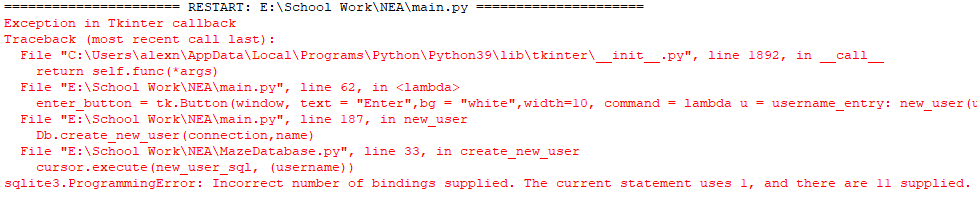
\includegraphics[scale=0.6]{Error - Username}}
\\
\vphantom{0}
\\
\color{mygrey}(Image 1)
\end{center}

\begin{center}
\fbox{
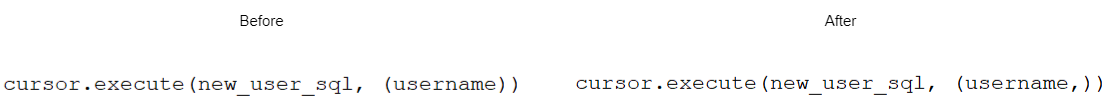
\includegraphics[scale=0.4]{Error - Username 2}}
\\
\vphantom{0}
\\
\color{mygrey}(Image 2)
\end{center}

%%%%%% maze generation
\vphantom{0}
\\
\begin{tabular}{|P{3.5cm}|P{0.8cm}|P{3cm}|P{4cm}|P{3cm}|P{3cm}| }
\hline
 Maze Generation was taking several magnitudes longer than it should have & 2 & Level 30 maze selected & Maze is generated in under 5 seconds & Generation takes more than a minute (See Image 3) & Weight Value for generation was too high (See Image 4/5) \\
\hline
\end{tabular}
\\
\begin{center}
\fbox{

\includegraphics[scale=1]{Error - Maze}}
\\
\vphantom{0}
\\
\color{mygrey}(Image 3)
\end{center}

\begin{center}
\fbox{
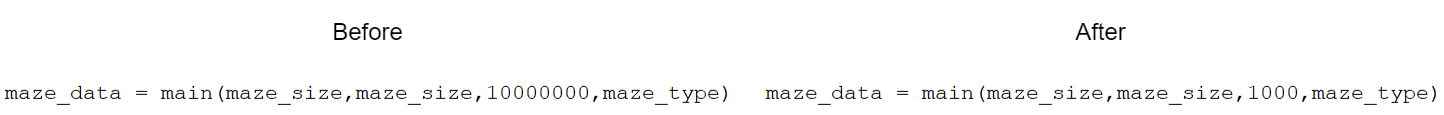
\includegraphics[scale=0.3]{Error - Maze 2}}
\\
\vphantom{0}
\\
\color{mygrey}(Image 4)
\end{center}

\begin{center}
\fbox{

\includegraphics[scale=1]{Error - Maze 3}}
\\
\vphantom{0}
\\
\color{mygrey}(Image 5)
\end{center}
%%%%%%%%%%%%%%%%%%


\clearpage
\section{Test Table (Post-Development)}
\begin{tabular}{|P{3cm}|P{1cm}|P{3cm}|P{3cm}|P{3cm}|P{1.2cm}|P{2cm}| }
\hline
 Objective & Test & Input & Expected Result & Actual Result & Passed & Comments \\
\hline
\textbf{GUI }&&&&&& \\
\hline
 Create New User & 1 & ExampleUser & New user is added to database & As expected & Yes & \\
\hline
Select User & 2 & Click on ExampleUser button & user\_id is set to the user id of ExampleUser & As expected & Yes & \\
\hline
 Select Maze Type & 3 & Normal Maze Type Selected & Maze Generated is of Normal Maze type & As expected & Yes & \\
\hline
 Select Maze Dimensions & 4 & Level 5 selected & Should generate a maze of size 8 by 8 & As expected & Yes & \\
\hline
 Input Maze of non-equal dimensions in custom maze screen & 5 & Entered dimensions of 16 by 5 & Should generate a maze of size 16 by 5 & As expected & Yes & \\
\hline
\textbf{Gameplay}&&&&&& \\
\hline
 Arrow Key Input & 6 & Every arrow key in turn & Should move in one of the four directions depending on arrow key pressed & As expected & Yes & Test was done in a maze without walls so all directions could be tested easily\\
\hline
 Collision Detection & 7 & Attempts to move through wall & Movement is not allowed & As expected & Yes & \\
\hline
 Win detection & 8 & Moves to the win position & Game ends, displaying "Maze Completed" screen & As expected & Yes & \\
\hline
\end{tabular}

%%%%%%%%%%%%%%%%%%%%%%%%%%

\clearpage
\part{New Evaluation}
\section{Were the objectives met?}
\subsection{Performative Maze Rendering}
I believe this objective has been met very well, as both sub-objectives ("Layer Based Rendering" and the "Ability to edit any given pixel on a given layer") have been implemented. The sixty frames per second minimum has also been certainly met with the program averaging ~2000 frames, however, the  fps calculation is admittely limited. If the time taken to execute a frame is recorded as 0 then the calcualtion cannot be performed as to avoid a zero division error. The code could also be compilied using something such as Cython. This means that the frame rate could be higher, though 2000 frames is certainly enough. The pixels on screen can also be any colour representable in the format (8-bit integer, 8-bit integer,8-bit integer), meaning there are 1,6581,375 possible colours. Currently, the main part of the rendering that could be improved is the dependency on outside libraries, specifically Pillow and Numpy, this would be the part of the program that I would seek to fix first. 

\subsection{Gameplay Mechanics}
The program is also capable of all the outlined gameplay features, it can read whatever key is currently being pressed on the keyboard as well as use the current maze coordinates to check what walls are around the player. However, the collision system used very specific to the project with it working entirely off the maze\_array. The program can also use said maze coordinates to see if the player is at the exit of the maze. Unfortunately, I think the gameplay can get monotonous and more mechanics would be helpful to break up the gameplay, these could be the timer/monsters mentioned in the analysis or something like tunnels that lead to another part of the maze. If there was also a cap on how big groups could get then the maze would instead be spilt into multiple smaller mazes with the tunnels used to connect them. Of course, there would need to be checks in place to make sure the maze was still solvable.

\subsection{Controllable Maze Generation}
In my opnion, similar to the Gameplay Mechanics, this objective has been met but ultimately more could be done. For example, the book used for research mentioned in the analysis ("Mazes for Programmers") talks about weaving (underpasses and bridges) which could have been an interesting and unique addition to the maze generation. In terms of storing the maze, I think the way of accessing a specific cell is implemented well (being utilized in the gameplay mechanics discussed above), with each index being analogous to that given cells coordinate. However, as discussed in the section about the maze\_array data structure, there could have been optimizations made to the way information about cell walls is stored.

\subsection{GUI}
I believe my GUI has everything I outlined as an objective for it. It has a user select screen, a maze type select screen and a level select screen. The user select screen also has a button leading to a user creation screen where a username can be input, however, it does lack the ability to delete users. On the maze typeselect screen there is two maze types avaliable as well as a custom
 maze option, leading to an options menu. Lastly there is the level select screen which features adjustable columns and adjustable number of levels overall. The text on the buttons is turned green when a level is completed, utilizing the database system evaluated below.

\clearpage
\subsection{System for storing users completed levels}
I think that the database system works well and it is utilized for various things, all discussed above. However, there is no ability to remove a user from the database, meaning any user created is permanent, though any given user's progress can be reset. Apart from pure functionality, its purpose was to demonstrate that I had the ability to use SQLite3 and I think it also does that well.

\section{Is the feedback from potential users met?}
I believe that I met some but not all of the points outlined in the "Potential Users Intial Feedback summary" section of the Analysis. There is certainly general patterns to the mazes, defined as different maze types but all mazes remain square. I also personally believe input feels nice, allowing the user to progress through the maze fast if they know where they are going, however, once or twice I overshot where I intended to stop. There is a custom maze screen, however, maze size is capped at 50 by 50, which is large but not stupidly so. Music and bloom were two suggestions I could not add, if I had more time I could have probably included the latter but I have little idea to how I could have implemented the former.

\section{What have I learnt?/What could I do better next time?}
During this project I have learnt a lot, specifically when it comes to rendering. While I was already interested in maze generation before the NEA, I had never done anything with rendering before. Even though my renderer doesn't iimplement many of the things I came across after the research stage (though it does do what it was made for), I still have that knowledge for projects I attempt in the future. Another thing I intend to do in future projects is more code upkeep, while ultimately I feel the technical solution is mostly fine when it comes to code upkeep, there could still be some obvious improvments made to the clarity of the current code. As discussed in both the "Gameplay Mechanics" and "Is the feedback from potential users met?" I would also have liked to add more gameplay features, with a timer being the first one of them I would implement. 

\section{Conclusion}
In conclusion, I believe my project fufills all of my originally outlined objectives and it is fully functional, however, there are certainly quite a few improvments that could be made. As specified in the "Performative Maze Rendering" section the part of the program I would fix first is the dependency on outside packages and then I would likey implement a timer alongside maze weaving. Overall however, I believe this project has gone well.

\clearpage

%%%%%%%%%%%%%%%%%%%%%%%%%%
\clearpage
\part{Appendix}
\section{main.py}
This script handles the creation of the UI as well as running the Maze Database, MazeGenerationNew and 
MazeRendererNew scripts.

\textcolor[RGB]{220,220,220}{\rule{\linewidth}{0.2pt}}
\begin{lstlisting}
def change_state(state):      

    des()
    if state == "start":    
        title = tk.Label(window, text = "\n Maze Game \n Version 2.0 \n", bg = "white", borderwidth=1, relief="groove").pack(fill = "x",pady=(250,20))
        enter_button = tk.Button(window, text = "Enter",bg = "white",width=30, command = lambda: change_state("username")).pack()
        exit_button = tk.Button(window, text = "Exit",width=30, bg = "white", fg = "red", command = lambda: exit()).pack(pady=3)
        if not installed:
            error_message = tk.Label(window,text="[PIL or Numpy not installed, PIL and Numpy are required for current version]",fg="red").pack(side="bottom",pady = 20)
    if state == "username": 
        title = tk.Label(window, text = "\n Accounts \n", bg = "white",  borderwidth=1, relief="groove").pack(fill = "x",pady=(20,100))
        top_seperator = tk.Canvas(window, height=50,width=0).pack()
        user_list = Db.get_list_of_users(connection)
        for i in range(0,len(user_list)): #Loads all the current users
            username_button = tk.Button(window,text=((user_list[i][1])[2:-1] + "\n" + "(#" + ("0" * (3-len(user_list[i][0]))) + user_list[i][0] + ")"),bg = "white",width=30,height=2)
            username_button.config(command = lambda u = user_list[i][0]: set_user_id(u,False))
            username_button.pack(pady=3)
        guest_button = tk.Button(window, text = "Play as Guest",bg = "white",width=30,height=2, command = lambda u = "guest": set_user_id(u,True)).pack(pady=3)
        create_new_button = tk.Button(window,text="+",bg = "white",width=10, command = lambda: change_state("new user")).pack(pady=3)
        back_button = tk.Button(window, text = "Back", command = lambda: change_state("start")).pack(side="bottom",pady=10)  
    elif state == "new user":   #New user screen
        title = tk.Label(window, text = "\n New User \n", bg = "white",  borderwidth=1, relief="groove").pack(fill = "x",pady=(20,100))
        username_text = tk.Label(window, text = "Username").pack(pady=(10,1))
        username_entry = tk.Entry(window,width=20)
        username_entry.pack()
        enter_button = tk.Button(window, text = "Enter",bg = "white",width=10, command = lambda u = username_entry: new_user(u)).pack(pady = 10)
        back_button = tk.Button(window, text = "Back", command = lambda: change_state("username")).pack(side="bottom",pady=10)  
    elif state == "maze select":    #Maze type select screen. Options are, Normal, Diamond and Custom
        if user_id != 0:
            completed = Db.get_list_of_completed_levels(connection,user_id)
        else:
            completed = [[],[]]
        title = tk.Label(window, text = "\n Maze Select \n", bg = "white",  borderwidth=1, relief="groove").pack(fill = "x",pady=(20,100))
        normal_maze_button = tk.Button(window, text = "\n  Normal-Style Maze  \n",bg = "white",relief = 'groove',width=30, command = lambda: create_levels(1,32,4,"Normal Maze","normal",completed)).pack(pady=(50,10))
        circular_maze_button = tk.Button(window, text = "\n Diamond Maze \n",bg = "white",relief = 'groove',width=30,command = lambda: create_levels(1,32,4,"Diamond Maze","diamond",completed)).pack(pady=10)
        custom_maze_button = tk.Button(window, text = "\n Custom Maze \n",bg = "white",relief = 'groove',width=30,command = lambda: change_state("custom maze")).pack(pady=10)
        reset_button = tk.Button(window, text = "Reset Progress",width=30, bg = "white",relief="groove",fg="red", command =  lambda: reset_progress()).pack(pady=50)        
        back_button = tk.Button(window, text = "Back", command = lambda: change_state("username")).pack(side="bottom",pady=10)      
    elif state == "custom maze":    #Custom maze creation screen
        first = tk.Frame(window)
        title_ = tk.Label(window, text = ("\n Custom Maze \n"), bg = "white", borderwidth = 1, relief = "groove").pack(fill = "x",pady=20)
        top_seperator = tk.Canvas(window, height=50,width=0).pack()
        #GENERATION
        generation_frame = tk.Frame(window,width=10,height=10)
        generation_frame.pack(side="left", anchor='n',padx=50)
        title_ = tk.Label(generation_frame, text = ("\n Generation \n"), bg = "white", borderwidth = 1,width = 100, relief = "groove").pack(pady=20)
        #Maze Type 
        maze_type_text = tk.Label(generation_frame, text = "Type").pack(padx=4,pady=(10,0))
        variable = tk.StringVar(generation_frame)
        variable.set("normal")
        maze_type_menu = tk.OptionMenu(generation_frame, variable, "normal","diamond")
        maze_type_menu.pack(pady=(0,10))
        #Width
        width_text = tk.Label(generation_frame, text = "Width").pack(padx=4)
        width_scale = tk.Scale(generation_frame, tickinterval=2, length=600, orient="horizontal",from_ = 2,to=50)
        width_scale.pack()
        #Height
        height_text = tk.Label(generation_frame, text = "Height").pack(padx=4)
        height_scale = tk.Scale(generation_frame, tickinterval=2, length=600, orient="horizontal",from_ = 2,to=50)
        height_scale.pack()
        #RENDERING
        render_frame = tk.Frame(window,width=10,height=10)
        render_frame.pack(side="right", anchor='n',padx=50)
        title_ = tk.Label(render_frame, text = ("\n Rendering \n"), bg = "white", borderwidth = 1,width = 100, relief = "groove").pack(pady=(20,5))
        #Cube Size
        cs_text = tk.Label(render_frame, text = "Cell Size").pack(padx=4,pady=(10,0))
        cs_entry = tk.Entry(render_frame, width=20)
        cs_entry.insert("end", '10')
        cs_entry.pack()
              
        generate_maze = tk.Button(window, text = "Generate",relief = 'groove', bg="white", command = lambda mt = variable, w = width_scale, h = height_scale, c = cs_entry: custom_maze(mt,h,w,c,"CUSTOM MAZE"))
        generate_maze.pack(pady=400)
        back_button = tk.Button(window, text = "Back", command = lambda: change_state("maze select")).pack(side="bottom",pady=10)


def create_levels(lower,upper,number_of_columns,title,maze_type,completed):
    des()
    first = tk.Frame(window)
    first.pack(side='top')
    side = first
    title_ = tk.Label(window, text = ("\n" + title + "\nSelect a level\n"), bg = "white", borderwidth = 1, relief = "groove").pack(in_ = first,fill = "x",pady=20)
    top_seperator = tk.Canvas(window, height=50,width=0).pack(in_ = side)
    dict_one = {
                "normal":0,
                "diamond":1
                }
    for i in range((lower),(upper+1)):
            text = str(i)                          
            try:
                if completed[dict_one[maze_type]].count(text) > 0:
                    fg = "green"
                    text += "\n(Complete)"
                else:
                    fg = "black"
            except:
                fg = "black"
            button = tk.Button(window, text=text, width = 10, relief = 'groove', bg = "white",fg = fg)
            button.config(command = lambda mt = maze_type, btn = button : load_maze(lower,upper,title,mt,dict_one[maze_type],btn))
            button.pack(in_ = side, side = "left", padx=10,pady=10)
            if (i%number_of_columns) == 0:
                middle = tk.Frame(window)
                middle.pack(side = "top")
                side = middle
    back_button = tk.Button(window, text = "Back", command = lambda: change_state("maze select")).pack(side="bottom",pady=10)

def load_maze(lower,upper,title,maze_type,btn):   #Generates the maze and then passes the data along with other parameters to the MazeRenderer script
    maze_size = int((btn['text']).replace("\n(Complete)","")) + 3
    if installed:        
        maze_data = main(maze_size,maze_size,1000,maze_type)
        dict_two = {
            "normal":[[len(maze_data[0])-1],[0],[0,len(maze_data)-1]],
            "diamond":[[len(maze_data[0])-1],[0],[0,len(maze_data)-1]]
            }
        win_pos_x = (dict_two[maze_type])[0]
        win_pos_y = (dict_two[maze_type])[1]
        start_pos = (dict_two[maze_type])[2]
        dimensions = alter_screen()
        won = play_maze(dimensions[0],dimensions[1],(str(maze_size) + " x " + str(maze_size)),10,win_pos_x,win_pos_y,start_pos,maze_data)
    else:
        won = True  #Maze auto-completes if PIL is not installed
    if won:
        if user_id != 0:
            Db.add_completed_level(connection,maze_size-3, maze_type,user_id)
    completed = Db.get_list_of_completed_levels(connection,user_id)
    create_levels(lower,upper,4,title,maze_type,completed)

def custom_maze(maze_type,width,height,cube_size,title):    #Same as the function above but for custom mazes
        width = int(width.get())
        height = int(height.get())
        cube_size = int(cube_size.get())
        maze_data = main(width,height,1000,maze_type.get())
        dimensions = alter_screen()
        play_maze(dimensions[0],dimensions[1],(str(width) + " x " + str(height)),cube_size,[len(maze_data[0])-1],[0],[0,len(maze_data)-1],maze_data)
        change_state('custom maze',True)

def set_user_id(username,guest):    #Sets the user ID
    global user_id
    if guest:
        user_id = 0
    else:
        user_id = username
    change_state("maze select")

def reset_progress():           #Resets the current users progress
    username = Db.delete_user(connection, user_id)
    Db.create_new_user(connection, username)
    change_state("maze select")

def new_user(user_entry_widget):    #Creates a new user named using the entered user name
    name = user_entry_widget.get()
    Db.create_new_user(connection,name)
    change_state("username")

def des(): #Deletes all current widgets in "window"
    widget_list = all_children(window)
    for item in widget_list:
        item.pack_forget()

def all_children(window): # This makes a list of all the current widgets
    list_one = window.winfo_children()
    for item in list_one:
        if item.winfo_children() :
            list_one.extend(item.winfo_children())
    return list_one

def alter_screen():     #Changes screen dimenions to make the rendering of the maze faster
    const = 2
    dimensions = [0,0]
    dimensions[0] = int(screen_width/const)
    dimensions[1] = int(screen_height/const)
    return dimensions
\end{lstlisting}

%%%%%%%%%%%%%%%%%%%%%%%%%%

\clearpage
\section{MazeDatabase.py}
Script for interaction with the maze.db for storing users and completed levels, utilizes SQL.

\textcolor[RGB]{220,220,220}{\rule{\linewidth}{0.2pt}}
\begin{lstlisting}
def main_database():    #Creates the database (if it wasn't already created) and establishes a connection to it 
    user_table = " CREATE TABLE IF NOT EXISTS users (
id integer PRIMARY KEY,
username text NOT NULL
); "
    completed_levels_table = " CREATE TABLE IF NOT EXISTS completedLevels (
id integer PRIMARY KEY,
normal_maze text,
diamond_maze text,
user_id integer NOT NULL,
FOREIGN KEY (user_id) REFERENCES users (id)
); " 
    connection = create_connection(r"Maze.db")
    if connection is not None:
        create_table(connection,user_table)
        create_table(connection,completed_levels_table)
    else:
        print("Database Connection Error")
    return connection

"DATABASES
Users table stores name and user_id + any additional information needed
CompletedLevels table stores the completed levels linked to the foreign key user_id and a primary key completed_id. There will be two columns, one for normal mazes, one for diamond mazes
the completed levels will be serialized as such (1#3#4#12...) and when the string is imported it will be split into a list."

def create_new_user(connection, username):
    #Create the new user
    new_user_sql = "INSERT INTO users(username) VALUES(?)"
    cursor = connection.cursor()
    cursor.execute(new_user_sql, (username,))
    user_id = cursor.lastrowid
    connection.commit()
    #Then create the sibling entry in the CompletedLevels table based of the generated user_id
    new_completed_levels_sql = "INSERT INTO completedLevels(normal_maze, diamond_maze, user_id) VALUES(?,?,?)"
    cursor = connection.cursor()
    cursor.execute(new_completed_levels_sql, ("","",user_id))
    connection.commit()

def delete_user(connection, user_id):
    sql = 'SELECT username FROM users WHERE id = ?'
    cursor = connection.cursor()
    cursor.execute(sql, (user_id))
    result = cursor.fetchall()
    #Delete user entry
    sql = 'DELETE FROM users WHERE id=?'
    cursor = connection.cursor()
    cursor.execute(sql, (user_id))
    connection.commit()
    #Delete completedLevels entry
    sql = 'DELETE FROM completedLevels WHERE user_id=?'
    cursor = connection.cursor()
    cursor.execute(sql, (user_id))
    connection.commit()
    return result[0][0]

def get_list_of_users(connection):
    user_list = []
    cursor = connection.cursor()
    cursor.execute("SELECT * FROM users")
    result = cursor.fetchall()
    for row in result:
        user_list.append((str(row)[1:-1]).split(','))
    return user_list

def add_completed_level(connection, level_number, maze_type, user_id):    #Uses the user id to alter the user's completed levels
    completed = get_list_of_completed_levels(connection, user_id)
    dict_one = {
                "normal":0,
                "diamond":1
                }
    formatted = ''
    for level_num in completed[dict_one[maze_type]]:
        print(level_num)
        formatted = formatted + level_num + "#"
    formatted = formatted + str(level_number)
    if maze_type == "normal":
        sql = "UPDATE completedLevels SET normal_maze = ? WHERE user_id = ?"
    elif maze_type == "diamond":
        sql = "UPDATE completedLevels SET diamond_maze = ? WHERE user_id = ?"
    cursor = connection.cursor()
    cursor.execute(sql,(formatted,user_id))

def get_list_of_completed_levels(connection, user_id):
    maze_find_sql = "SELECT normal_maze, diamond_maze FROM completedLevels WHERE user_id = ?"
    cursor = connection.cursor()
    cursor.execute(maze_find_sql,(user_id))
    result = cursor.fetchall()
    return [(result[0][0]).split('#'),(result[0][1]).split('#')]

def create_connection(db_file):
    connection = None
    try:
        connection = sqlite3.connect(db_file)
    except Error as e:
        print(e)
    return connection

def create_table(connection, create_table):
    try:
        cursor = connection.cursor()
        cursor.execute(create_table)
    except Error as e:
        print(e)
\end{lstlisting}


%%%%%%%%%%%%%%%%%%%%%%%%%%

\clearpage
\section{MazeGenerationNew.py}
Uses Kruskal’s algorithm paired with a generated weight array to create the maze.

\textcolor[RGB]{220,220,220}{\rule{\linewidth}{0.2pt}}
\begin{lstlisting}
def intialize_array(width,height):
    #Intialize the array
    maze_array = []
    for x in range(0,width):
        maze_array.append([])
        for y in range(0,height):
            maze_array[x].append([1,1,1,1]) #Add a blank cell with all four walls to create an array that will be altered to generate a maze, this array is the data we return
    return maze_array

def generate_random_walls(height,width):    #Random walls for testing maze renderer
    #Intialize the array
    maze_array = []
    temp_list = [0,0,0,0,0,0,1]
    for x in range(0,width):
        maze_array.append([])
        for y in range(0,height):
            maze_array[x].append([random.choice(temp_list),random.choice(temp_list),random.choice(temp_list),random.choice(temp_list)])
    return maze_array

def kruskals_algorithim(weight_group_array,width,height,max_weight): #Based loosely on the algorithim as described in "Mazes for Programmers"
    maze_array = intialize_array(width,height)
    group_designation = 1                                                                                                                                           
    temp_list_empty = False
    while not all_in_one_group(weight_group_array,height,width) and not temp_list_empty: #Only ends loop when no new corridors can be checked and all the corriders are in the same group
        temp_list = lowest_values_pos(weight_group_array,width,height,max_weight+1)
        if temp_list == []:
            temp_list_empty = True
        else:
            dict_one = {
                0:[0,-1,1],
                1:[0,1,0],
                2:[-1,0,3],
                3:[1,0,2]
                }
            for pos in temp_list:
                can_connect = True
                difference = dict_one[pos[2]]
                current_pos_group = (weight_group_array[pos[0]][pos[1]])[4]                
                try:
                    if pos[0]+difference[0] == -1 or pos[1]+difference[1] == -1:
                        error = pos[100]
                    connected_pos_group = (weight_group_array[pos[0]+difference[0]][pos[1]+difference[1]])[4]
                    if current_pos_group == 0:
                        if connected_pos_group == 0:
                            (weight_group_array[pos[0]][pos[1]])[4] = group_designation
                            (weight_group_array[pos[0]+difference[0]][pos[1]+difference[1]])[4] = group_designation
                            group_designation += 1
                        else:
                            (weight_group_array[pos[0]][pos[1]])[4] = (weight_group_array[pos[0]+difference[0]][pos[1]+difference[1]])[4]
                    else:
                        if current_pos_group == connected_pos_group:
                            can_connect = False
                        elif connected_pos_group == 0:
                            (weight_group_array[pos[0]+difference[0]][pos[1]+difference[1]])[4] = current_pos_group
                        elif connected_pos_group != 0:
                            group_pos = get_all_in_group(weight_group_array,width,height,connected_pos_group)
                            for pos2 in group_pos:
                                (weight_group_array[pos2[0]][pos2[1]])[4] = current_pos_group
                    if(can_connect):
                        (maze_array[pos[0]][pos[1]])[pos[2]] = 0
                        (maze_array[pos[0]+difference[0]][pos[1]+difference[1]])[difference[2]] = 0
                    (weight_group_array[pos[0]][pos[1]])[pos[2]] = max_weight+2
                    (weight_group_array[pos[0]+difference[0]][pos[1]+difference[1]])[difference[2]] = max_weight+2
                except IndexError:
                    (weight_group_array[pos[0]][pos[1]])[pos[2]] = max_weight+2
                    if (weight_group_array[pos[0]][pos[1]])[4] == 0:
                        (weight_group_array[pos[0]][pos[1]])[4] = group_designation
                        group_designation += 1
    return maze_array

def lowest_values_pos(wg_array,width,height,compared_to):   #Finds all the connections in the maze with the lowest weight value
    temp_list = []
    for x in range(0,width):
        for y in range(0,height):
            for i in range(0,4):
                if wg_array[x][y][i] < compared_to:
                    compared_to = wg_array[x][y][i]
                    temp_list = []
                    temp_list.append([x,y,i])
                elif wg_array[x][y][i] == compared_to:
                    temp_list.append([x,y,i])
    return temp_list

def get_all_in_group(wg_array,width,height,group):  #Gets the positions of all the cells that have the group specified
    temp_array = []
    for x in range(0,width):
        for y in range(0,height):
            if (wg_array[x][y])[4] == group:
                temp_array.append([x,y])
    return temp_array

def all_in_one_group(wg_array,height,width):    #Checks to see if every cell is in a singular group (a.k.a every cell can be reached from any other cell)
    returned = True
    first_group = "null"
    for x in range(0,width):
        for y in range(0,height):
            temp = (wg_array[x][y])[4]
            if first_group == "null":
                first_group = temp
            if temp != first_group or temp == 0:
                returned = False                
    return returned

def generate_walled_maze(width,height,max_weight):
    weight_group_array = []                 
    for x in range(0,width):
        weight_group_array.append([])
        for y in range(0,height):
            weight_group_array[x].append([random.randint(1,max_weight),random.randint(1,max_weight),random.randint(1,max_weight),random.randint(1,max_weight),0])   #Create a "sister" array that stores the weight values and group of each cell
    maze_array = kruskals_algorithim(weight_group_array,width,height,max_weight)    #Use the weight array to generate an actual maze
    return maze_array

def generate_diamond_maze(width,height,max_weight):
    weight_group_array = []
    for x in range(0,width):
        weight_group_array.append([])
        for y in range(0,height):
            weight_group_array[x].append([random.randint(1,max_weight),random.randint(1,max_weight),random.randint(1,max_weight),random.randint(1,max_weight),0])
    #Manipulate the weight group array to make the algorithim generate a diamond maze with random gaps in the walls
    center_of_maze = [int(width/2),int(height/2)]
    pos_to_change = center_of_maze
    counter = 1
    circling = True
    translate_to_displacement = {
        1:[0,1],
        2:[1,0],
        3:[0,-1],
        0:[-1,0]
        }
    translate_to_wall_index = {
        1:2,
        2:1,
        3:3,
        0:0
        }
    while circling:
        modded_counter = counter % 4
        displacement = translate_to_displacement[modded_counter]
        wall_index = int(translate_to_wall_index[modded_counter])
        length_counter = counter // 2 + (counter % 2)
        for i in range(1,length_counter):
            #Check to see if current cell is within maze
            if pos_to_change[0] > width-1 or pos_to_change[1] > height-1:
                pass
            else:
                #If it is then remove the wall leading to the new cell
                weight_group_array[pos_to_change[0]][pos_to_change[1]][wall_index] = counter
            #Move into the new cell
            pos_to_change = [pos_to_change[0]+displacement[0],pos_to_change[1]+displacement[1]]
        counter += 1
        #Fail state check
        if pos_to_change[0] > width and pos_to_change[1] > height:
            circling = False
    weight_group_array[center_of_maze[0]][center_of_maze[1]] = [0,0,0,0,0] #Remove all walls from center
    maze_array = kruskals_algorithim(weight_group_array,width,height,max_weight)
    return maze_array 
\end{lstlisting}

%%%%%%%%%%%%%%%%%%%%%%%%%%

\clearpage
\section{Window.py}
Uses tkinter, NumPy and pillow (a fork of PIL (Python Imaging Library)) to create layered editable images on screen. Using tkinter it also handles input, unfortunately the window needs to be clicked on for input to be registered.

\textcolor[RGB]{220,220,220}{\rule{\linewidth}{0.2pt}}
\begin{lstlisting}
class Window():
    pixel_scale = 1
    last_key_pressed = None
    
    def __init__(self, height, width, default_colour, title):   #Creates the intial image and sets intial values
        self.height = int(height)
        self.width = int(width)
        self.title = title
        self.default_colour = default_colour
        self.window = create_tkinter_window(self.height, self.width, self.title)
        self.screen = create_canvas(self.window)
        self.layers = []
        self.layers.append(self.Layer(self,self.height,self.width,self.default_colour)) #Create the background layer

    class Layer():  #Layer Objects

        def __init__(self,window,height,width,default_colour):
            self.height = height
            self.width = width
            self.default_colour = default_colour
            self.layer_num = len(window.layers)
            self.array = create_image_array(height,width,default_colour)
            self.generated_image = ImageTk.PhotoImage(master = window.screen,image=Image.fromarray(self.array))
            self.image = window.screen.create_image(width,height,image=self.generated_image)

    def move_layer(self,new_coords,layer_num = 0):  #Moves a layer to a given position
        #Get Current Top Left of layer Coords
        old_coords = self.screen.coords(self.layers[layer_num].image)
        old_coords[0] = old_coords[0] - (self.layers[layer_num].height/2)
        old_coords[1] = old_coords[1] - (self.layers[layer_num].width/2)
        #Move to new position
        self.screen.move(self.layers[layer_num].image,new_coords[0] - old_coords[0],new_coords[1] - old_coords[1])

    def delete_layer(self,layer):
        self.screen.delete(self.layers[layer].image)
        self.layers.pop(layer) 

    def reset(self, layer_num = 0):    #Resets the entered layer, used so the line below doesn't need to be typed everytime
        self.layers[layer_num].array = create_image_array(self.layers[layer_num].height,self.layers[layer_num].width,self.layers[layer_num].default_colour)

    def set_pixel(self, coords, colour, layer_num=0): #Change a pixel in the image array
        coords[0] = (coords[0] * self.pixel_scale) - (self.pixel_scale - 1)
        coords[1] = (coords[1] * self.pixel_scale) - (self.pixel_scale - 1)
        for x in range(coords[0],coords[0]+self.pixel_scale):
            for y in range(coords[1],coords[1]+self.pixel_scale):
                try:
                    self.layers[layer_num].array[y,x] = colour
                except IndexError:
                    pass   

    def update(self, layer_num = 0):   #Updates an entered layer
        try:
            self.layers[layer_num].generated_image = ImageTk.PhotoImage(master = self.screen,image=Image.fromarray(self.layers[layer_num].array)) #Generate a updated image from the image array
            self.screen.itemconfig(self.layers[layer_num].image, image = self.layers[layer_num].generated_image)    #Applies the generated image
        except IndexError:
            print("Invalid Layer")
        self.window.update()

    def init_input(self):                   #Input created using tkinter, last key pressed = key pressed that frame
        def on_key_press(event):
            self.last_key_pressed = event.char
            if self.last_key_pressed == '\boxempty':
                self.last_key_pressed = 'esc'
        def on_key_up(event):
            self.last_key_pressed = None
        self.window.bind('<KeyPress>', on_key_press)
        self.window.bind('<KeyRelease>', on_key_up)

    def set_fullscreen(self, boolean):  #Turns fullscreen on and off based on boolean
        self.window.overrideredirect(True)
        self.window.overrideredirect(False)
        self.window.attributes('-fullscreen',boolean)
        self.screen.pack(fill="both", expand=True)

    def set_pixel_scale(self, num): #Used to change the pixel scale
        self.pixel_scale = num

    def quit(self):                             #Quits window
        for i in range(0,len(self.layers)):
            self.reset(i)
        self.window.destroy()
        del self

def create_tkinter_window(height, width, title):    #Creates a tkinter window
    window = tk.Tk()
    window.title(title)
    window.geometry(str(width) + "x" + str(height))
    #window.overrideredirect(1) #Removes the Titlebar
    return window

def create_canvas(tkinter_window):  #Creates a tkinter canvas
    canvas = tk.Canvas(tkinter_window, bg="black")
    canvas.pack(fill="both",expand=True)
    return canvas

def create_image_array(height,width,colour): #Creates the intial image array
    image_array = np.zeros([height+1,width+1,3],dtype=np.uint8)
    image_array.fill(colour)
    return image_array
\end{lstlisting}

%%%%%%%%%%%%%%%%%%%%%%%%%%

\clearpage
\section{MazeRendererNew.py}
Used when actually playing a maze, mainly used to implement the Window.py script to correctly draw the maze but also handles collision detection and a check to see if the player has won.

\textcolor[RGB]{220,220,220}{\rule{\linewidth}{0.2pt}}
\\
\begin{lstlisting}
\end{lstlisting}
\begin{lstlisting}
#GAME LOGIC
def play_maze(width,height,title,cube_size,win_pos_x,win_pos_y,start_pos,maze_data):
    #A cube_size of two and below will cause the squares to be too small to be properly represented properly on any pixelated screen, hence, 3 is the lowest the function allows
    if cube_size < 3: cube_size = 3 
    screen = Window.Window(height,width,0,"Test Window")
    screen.set_fullscreen(True)
    screen.init_input()
    screen.update()
    temp = 0 #Temporary Variable to manage progress of stand-in progress bar
    delta_time = 0
    fps = 0
    time_to_close = 1.5
    add_to_y = 0
    add_to_x = 0
    loading = True
    first_frame = True
    running = True
    position_set_to = [1,0]
    move_dir = ""
    player_pos = start_pos
    active_last_frame = True
    check_walls = True
    to_return = False
    ending = True
    drawing_per_frame = False
    input_confirmed = False
    input_delay = 0    
    while running:
        #Anything in this loop is run every frame
        start_time = time.time() #For measuring execution time, it is used for debug, testing program speed and the calculation of delta_time        
        #Input
        if input_delay <= 0:
            if screen.last_key_pressed != None and input_confirmed:
                if screen.last_key_pressed == 'esc':
                    running = False
                if screen.last_key_pressed == 'a':
                    add_to_x = -1
                    move_dir = "left"
                elif screen.last_key_pressed == 'd':
                    add_to_x = 1
                    move_dir = "right"
                elif screen.last_key_pressed == 'w':
                    add_to_y = -1
                    move_dir = "up"
                elif screen.last_key_pressed == 's':
                    add_to_y = 1
                    move_dir = "down"
                else:
                    move_dir = ""
                #Checks to make sure player can't go outside the maze
                if position_set_to[0] + add_to_x < 0 or position_set_to[0] + add_to_x > len(maze_data[0])-1:
                    add_to_x = 0
                    check_walls = False
                if position_set_to[1] + add_to_y < 0 or position_set_to[1] + add_to_y > len(maze_data)-1:
                    add_to_y = 0
                    check_walls = False
                #Checks to see if there is a wall in the players way
                if(wall(maze_data,[position_set_to[0] + add_to_x,position_set_to[1] + add_to_y],player_pos,move_dir)) and check_walls:
                    add_to_y = 0
                    add_to_x = 0
                check_walls = True
                input_confirmed = False
            else:
                position_set_to = player_pos
                add_to_y = 0
                add_to_x = 0
                input_confirmed = True
                input_delay = 0.1        #The time between moves
        else:
            input_delay -= delta_time
        #Game Code
        if debug:
            print(str(round((time.time() - start_time)*1000,1)) + "ms") #Prints execution time (per frame) to console
            print(temp)
        if loading:
            if temp >= 1:
                loading = False
                screen.reset()
            else:
                if temp == 0:
                    #Create Title
                    text("Maze Game",10,[0,-height/4],white,screen,[width,height])
                    time.sleep(0.1)
                progress_bar(width/2,temp,screen,[0,height/4],[width,height])  #This is a stand-in progress bar to test how it would look, the real one's progression would be based on the maze generation progression
                temp += 1 * delta_time                                  #currently the maze generates before the progress bar is shown and the maze is rendered after (To make it properly linked to maze generation
        elif not loading:                                               #the progress bar would have to be called from the MazeGenerationNew script)
            if first_frame == True:                
                first_frame = False            
                maze_width = (len(maze_data) * (cube_size-1))+1
                maze_height = (len(maze_data[0]) * (cube_size-1))+1
                if drawing_per_frame:
                    x = 0
                    y = 0
                else:
                    draw_maze([maze_height,maze_width],[width,height], cube_size,[win_pos_x,win_pos_y], screen, maze_data)
                #Create Maze Title
                text(title,3,[0,-((((len(maze_data) * (cube_size-1))+1)/2)+15)],white,screen,[width,height])
                #Instantiate Player
                player_pos = draw_player(True,cube_size,screen,player_pos,maze_width,maze_height,[width,height])  
                position_set_to = player_pos
            else:
                if won(player_pos,win_pos_x,win_pos_y):#[len(maze_data[0])-1,0]):
                    if ending:
                        time.sleep(0.4) #Halts the game for a very short amount of time to make the transition to the end screen feel less abrupt
                        screen.delete_layer(1) 
                        screen.reset()                    
                        text("Maze Completed",10,[0,0],white,screen,[width,height])
                        text("#",5,[0,-50],white,screen,[width,height])
                        ending = False
                    if time_to_close < 0:
                        to_return = True
                        running = False
                    else:
                        time_to_close -= delta_time
                else:
                    if drawing_per_frame:
                        draw_maze_per_cell([maze_height,maze_width], [x,y], [width,height], cube_size, [win_pos_x,win_pos_y], screen, maze_data)
                        x += 1
                        if x == len(maze_data[y]):
                            x = 0
                            y += 1
                        if y == len(maze_data):
                            drawing_per_frame = False                  
                    player_pos = draw_player(False,cube_size,screen,[player_pos[0]+add_to_x,player_pos[1]+add_to_y],maze_width,maze_height,[width,height])
                    screen.update(layer_num = 1)
        delta_time = time.time() - start_time #delta_time is the time the program took to execute the last frame
        try:
            fps = 1/delta_time         
        except:
            fps = '#'
    screen.quit()
    return to_return
        
#CHECKS
def won(player_pos,win_pos_x,win_pos_y): #Compares player position to entered position
    if player_pos[0] in win_pos_x and player_pos[1] in win_pos_y:
        return True
    else:
        return False

def wall(maze_data,position_to_set_to,player_pos,move_dir): #Checks to see if there is a wall blocking the players way when they attempt to move
    if move_dir == "":
        return True
    dict_one = {
        "left":[0,1],
        "right":[1,0],
        "up":[2,3],
        "down":[3,2]
        }
    if (maze_data[player_pos[1]][player_pos[0]])[(dict_one[move_dir])[0]] == 1 or (maze_data[position_to_set_to[1]][position_to_set_to[0]])[(dict_one[move_dir])[1]] == 1:
        return True
    else:
        return False

#RENDERING
def draw_maze_per_cell(maze_dimensions, coords_to_draw, window_dimensions, cube_size, win_pos, screen, maze_data):  #Draw maze cell per frame
    offsetx = coords_to_draw[0] * (cube_size-1)
    offsety = coords_to_draw[1] * (cube_size-1)
    draw_rectangle([(0-(maze_dimensions[0]/2)+offsetx),((0-maze_dimensions[1]/2)+offsety)],cube_size,cube_size,False,white,screen,window_dimensions,0,maze_data[coords_to_draw[1]][coords_to_draw[0]])
    if won([coords_to_draw[0],coords_to_draw[1]],win_pos[0],win_pos[1]):
        draw_rectangle([(0-(maze_dimensions[0]/2)+offsetx+2),((0-maze_dimensions[1]/2)+offsety+2)],cube_size-4,cube_size-4,True,green,screen,window_dimensions,0)

def draw_maze(maze_dimensions, window_dimensions, cube_size, win_pos, screen, maze_data):   #Draw maze all at once
    offsetx = 0
    offsety = 0
    for y in range(0,len(maze_data)):
        for x in range(0,len(maze_data[y])):
            draw_rectangle([(0-(maze_dimensions[0]/2)+offsetx),((0-maze_dimensions[1]/2)+offsety)],cube_size,cube_size,False,white,screen,window_dimensions,0,maze_data[y][x])
            if won([x,y],win_pos[0],win_pos[1]):
                draw_rectangle([(0-(maze_dimensions[0]/2)+offsetx+2),((0-maze_dimensions[1]/2)+offsety+2)],cube_size-4,cube_size-4,True,green,screen,window_dimensions,0)
            offsetx += cube_size-1
        offsety += cube_size-1
        offsetx = 0
    screen.update()   

def draw_player(first_pos,cube_size,screen,position,maze_width,maze_height,window_dimensions): #Draws the player in the center of a square, indicated by x and y coordinates
    player_size = (cube_size * 0.6)-1
    if first_pos:
        screen.layers.append(screen.Layer(screen,int(player_size),int(player_size),255))
    #Move the layer to the correct position
    new_pos = find_center_of_square(maze_width,maze_height,cube_size,position)
    new_pos[0] = int(window_dimensions[0]) + new_pos[0] 
    new_pos[1] = int(window_dimensions[1]) + new_pos[1]
    screen.move_layer(new_pos,layer_num=1)
    return position

def progress_bar(width,progress,screen,offset,window_dimensions): #Generates a progress bar in the center of the screen, however, it's position can be shifted using the offset
    center = [0+offset[0],0+offset[1]]
    #Draw progress bar shell
    draw_rectangle([int(center[0]-width/2),center[1]],width,15,False,white,screen,window_dimensions,0,1)
    #Draw actual progress
    draw_rectangle([int(center[0]-width/2)+2,center[1]+2],int((width-4)*progress),11,True,white,screen,window_dimensions,0)
    screen.update()

def text(text,text_size,offset,colour,screen,window_dimensions,layer_num = 0):        #Draws entered text on screen in the font defined in 'font.txt', by default it is drawn in the center, however, this can be altered by entering an offset
    text_dict = {                                                       
        "a":0,"A":0,"b":1,"B":1,"c":2,"C":2,"d":3,"D":3,"e":4,"E":4,
        "f":5,"F":5,"g":6,"G":6,"h":7,"H":7,"i":8,"I":8,"j":9,"J":9,
        "k":10,"K":10,"l":11,"L":11,"m":12,"M":12,"n":13,"N":13,"o":14,"O":14,
        "p":15,"P":15,"q":16,"Q":16,"r":17,"R":17,"s":18,"S":18,"t":19,"T":19,
        "u":20,"U":20,"v":21,"V":21,"w":22,"W":22,"x":23,"X":23,"y":24,"Y":24,
        "z":25,"Z":25," ":26,"1":27,"2":28,"3":29,"4":30,"5":31,"6":32,"7":33,
        "8":34,"9":35,"0":36,"#":37
        }   #Maps a line in the text file to a character
    text_list = split(text)
    text_width = 0
    text_height = 5 * text_size
    offsetx = 0
    offsety = 0
    offset_character = 0
    for i in text_list:
        character_data = split_int(font[text_dict[i]])
        text_width += (int((len(character_data)*text_size)/5) + (1*text_size))
    for i in text_list:
        character_data = split_int(font[text_dict[i]])
        for y in range(0,5):
            for x in range(0,int(len(character_data)/5)):
                if character_data[(y*int(len(character_data)/5))+x] == 0:
                    pass
                else:
                    draw_rectangle([(-text_width/2)+offsetx+offset_character+(offset[0]),(-text_height/2)+offsety+(offset[1])],text_size,text_size,True,colour,screen,window_dimensions,layer_num)
                offsetx += text_size
            offsety += text_size
            offsetx = 0
        offset_character += (text_size * (len(character_data)/5))+(1 * text_size)
        offsety = 0
    screen.update()
        
def draw_rectangle(startpos,width,height,fill,colour,screen,window_dimensions,layer_num,*args): #Draws a rectangle based around 0,0 (screen center), for best use don't redraw things that are already drawn (i.e. stagnant sprites, like the maze)
    width = alter_to_fit_scale(width)
    height = alter_to_fit_scale(height)
    for i in range(0,len(startpos)):
        startpos[i] = alter_coords_to_fit_scale(startpos[i],int((window_dimensions[i])/2))
    if fill:
        for x in range(startpos[0],startpos[0]+width):
            for y in range(startpos[1],startpos[1]+height):
                screen.set_pixel([x,y],colour)
    if not fill:
        list_one = []
        if isinstance(args[0], int):
            for i in range(0,4):
                list_one.append(args[0])
        else:
            list_one = args[0]
        for x in range(startpos[0],startpos[0]+width):
            for y in range(startpos[1],startpos[1]+height):
                if (x in range(startpos[0]+list_one[0],startpos[0]+width-list_one[1])) and (y in range(startpos[1]+list_one[2],startpos[1]+height-list_one[3])):
                    pass
                else:
                    screen.set_pixel([x,y],colour,layer_num = layer_num)

#CONVERTORS                    
def find_center_of_square(maze_width,maze_height,cube_size,pos): #Converts x and y coords to pixel measurments so that the player can be properly positioned 
    x = pos[0]                                                   
    y = pos[1]
    pos_in_pixels = [(0-(maze_height/2)+(cube_size-1)*x)+(0.2*cube_size),(0-(maze_width/2)+(cube_size-1)*y)+(0.2*cube_size)]
    return pos_in_pixels

def alter_to_fit_scale(value): #Alters any variable to fit game scale    
    return int(value*scale)

def alter_coords_to_fit_scale(value,full): #Makes coords relative to the center and fits them to game scale   
    return int(full + (value*scale))

#OTHER
def split(word):                    #Splits a string into characters, used when drawing text
    return [char for char in word]

def split_int(word):                    #Splits a set of ints into characters
    word = word.replace(" ","")
    word = word.replace("\n","")
    return [int(char) for char in word]

def pythag(a,b):                #Intended to be used to help create the circle of visibilty around the player, not actually implemented
    return ((a*a)+(b*b))**0.5
\end{lstlisting}

\clearpage
\section{External Libraries installation guide}
All commands must be run in the windows command line
\subsection{PIP}
PIP comes pre-installed with most versions of python and so it is unlikely you'll have to install it. If you do have to install it, the installation guide is here: 
\begin{center}
\url{https://pip.pypa.io/en/stable/installing/}
\end{center}
\subsection{Pillow}
Pillow is a fork of PIL and is used in the rendering part of the project, to install the following commands must be run
\begin{lstlisting}
python3 -m pip install --upgrade pip
python3 -m pip install --upgrade Pillow
\end{lstlisting}
The first checks to see if pip is up to date and the second actually installs Pillow. These commands come from the Pillow website, shown here:
\begin{center}
\url{https://pillow.readthedocs.io/en/stable/installation.html}
\end{center}
\subsection{numpy}
Alongside Pillow numpy must also be installed, if pip has already been checked to see if it is up to date then only the following command needs to be run
\begin{lstlisting}
python3 -m pip install --upgrade numpy
\end{lstlisting}
otherwise, run both commands below
\begin{lstlisting}
python3 -m pip install --upgrade pip
python3 -m pip install --upgrade numpy
\end{lstlisting}
The numpy website link is below, if it is needed
\begin{center}
\url{https://numpy.org/install/l}
\end{center}



\end{document}